\documentclass[11pt,reqno]{amsart}

\usepackage[margin=1in]{geometry}
\usepackage{amsmath,amssymb,amsthm,mathtools}
\usepackage{booktabs,array,multirow,longtable}
\usepackage{enumitem}
\usepackage{tikz}
\usetikzlibrary{calc,positioning,arrows.meta,decorations.pathreplacing,shapes.geometric}
\usepackage[colorlinks=true,linkcolor=blue!60!black,citecolor=green!45!black,urlcolor=blue!60!black]{hyperref}

\theoremstyle{plain}
\newtheorem{theorem}{Theorem}[section]
\newtheorem{lemma}[theorem]{Lemma}
\newtheorem{proposition}[theorem]{Proposition}
\newtheorem{corollary}[theorem]{Corollary}

\theoremstyle{definition}
\newtheorem{definition}[theorem]{Definition}
\newtheorem{construction}[theorem]{Construction}

\theoremstyle{remark}
\newtheorem{remark}{Remark}[section]

\newcommand{\FEG}{\mathcal{F}_{\mathrm{EG}}}
\newcommand{\Vatt}{V_{\mathrm{att}}}
\newcommand{\tw}{\operatorname{tw}}
\newcommand{\EG}{\text{Erd\H{o}s--Gy\'arf\'as}}
\emergencystretch=1.5em
\DeclareRobustCommand{\_}{\ifmmode\text{\textunderscore}\else\textunderscore\allowbreak\fi}

\title[Erd\H{o}s--Gy\'arf\'as for Claw-Free Graphs via 2D Dyadic Packing]{%
Erd\H{o}s--Gy\'arf\'as for 2-Cycle, Sublinear-Circumference,\\
and Bowtie Claw-Free Graphs via Sub-Unit\\
2D Dyadic $L_\infty$-Packing}

\author{Seth Rehwaldt}
\date{\today}

\begin{document}

\begin{abstract}
The \EG{} conjecture (1995) asserts that every finite simple graph with minimum degree at least $3$ contains a simple cycle whose length is a power of two. While the conjecture is settled for graphs of sufficiently large constant average degree and for claw-free graphs with $\delta(G) \ge 4$ (Shauger, 1998) or planar claw-free graphs (Daniel--Shauger, 2001), the general sparse claw-free regime $\delta(G) \ge 3$---even for cubic claw-free graphs, which after excluding $C_4$ (e.g., $K_4$, which has no simple cubic triangle quotient) reduce to triangle-replaced simple cubic graphs $G = T(H)$---remains open.

We establish four main theorems in pure discrete combinatorics (with zero topological axioms), anchored by a sub-unit-constant two-dimensional dyadic $L_\infty$-packing theorem:
\begin{enumerate}[label=(\arabic*),leftmargin=2.2em]
  \item \textbf{Sub-Unit 2D Dyadic $L_\infty$-Packing:} Let $\FEG := \{L \ge 3 : [2L, 3L] \text{ avoids powers of } 2\}$. For every $W_1, W_2 \ge 0$ and every same-parity subset $S \subset [0, W_1] \times [0, W_2]$ with \emph{no diagonal collisions} ($|u_1 - u_2| \neq |v_1 - v_2|$ for distinct $(u_1, v_1), (u_2, v_2) \in S$) and $\max(|u_1 - u_2|, |v_1 - v_2|) + 2 \in \FEG$,
  \[
    |S| \;\le\; \frac{3}{5}\bigl((W_1 + 2)(W_2 + 2)\bigr)^{123/256}.
  \]
  \item \textbf{All 2-Cycle Cubic Claw-Free Graphs:} Every finite nonempty simple cubic claw-free graph whose triangle quotient $H$ admits a spanning $2$-factor consisting of two cycles (arbitrary dyadic block ratios, arbitrary chords, arbitrary parity/non-Hamiltonicity) contains a power-of-two cycle.
  \item \textbf{Universal Polynomial-$k$-Cycle, Sublinear Circumference, Sturmian, and Matching-Complement Theorems:} For any simple cubic graph $H$ whose triangle replacement $G = T(H)$ avoids all dyadic cycles (equivalently, every simple cycle length of $H$ lies in $\FEG$), every pair of vertex-disjoint cycles $C_1, C_2$ of lengths $x \le y$ has at most $\frac{12}{5}(y + 2)^{123/128}$ inter-cycle bridges, closing all $k$-cycle spanning $2$-factors with $k \le (n/2^{97})^{5/133}$ (and equal-block $k \in \{3, 4, 5\}$ at $M \ge 2^{36}, 2^{51}, 2^{62}$). For any cycle $C$ of length $y$ in $H$ ($n = |V(H)|$) whose complement $H - V(C)$ is covered by $m \ge 1$ vertex-disjoint paths, $y \ge \max(2^{97} m^{128/5},\, 25 n^{128/133})$ forces a dyadic cycle in $G = T(H)$; thus whenever a longest cycle $C$ of $H$ has complement covered by $m$ paths with $m$ fixed (or $m = o(n^{5/128})$), dyadic-cycle avoidance forces $|V(C)| = o(n)$ and hence $c(G) = 3|V(C)| = o(|V(G)|)$, breaking the linear circumference barrier for such families. Unconditionally, $c(G) \ge \frac{17}{18}|V(G)|$ (and $c(G) \ge \frac{15}{16}|V(G)|$ when $H$ is bipartite), or any cycle $C \subset H$ with $\Delta(H - V(C)) \le 1$, forces a dyadic cycle.
  \item \textbf{General $\Delta \le 4$, $\delta \ge 3$ Bowtie Claw-Free Reductions, $\bar{d} \ge 7/2$, $\tw(H/B) \le 3$, Order $\ge 120$, and Tier-1 Hamiltonian All-Chord-$B$:} Every $C_4$-free claw-free graph with $\delta(G) \ge 3$ and $\Delta(G) \le 4$ has representation $G \cong T(H)/B$ with exact lift window $[2L - k, 3L - k - m]$. In any dyadic-cycle-free graph, the bowtie subgraph $H_B$ is a spanning forest whose every tree component is induced in $H$, $F = H/H_B$ is simple, $\bar{d}(G) < \frac{7}{2}$ (closing all $4$-regular claw-free graphs), and cubic dyadic bounds transfer via $2^K \to 2^{K+1}$. A $15$-line Universal $3$-Tree Lemma shows every $C_4$-free independent-bowtie claw-free graph $G \cong T(H)/B$ ($\delta \ge 3, \Delta \le 4$) with $\tw(H/B) \le 3$ contains $C_8$ \emph{or} $C_{16}$ (so every such graph contains $C_4, C_8,$ or $C_{16}$), sharp for $C_{16}$ vs.\ $C_8$ via an explicit $39$-vertex non-planar $K_5$-minor witness $G_{39} = T(H_{14})/B$ with width-$3$ quotient $F_{11} = H_{14}/B$. Every dyadic-cycle-free independent-bowtie claw-free graph ($\delta \ge 3, \Delta \le 4$) with $4$-regular quotient $F$ satisfies $|V(F)| \ge 24$ and $|V(G)| \ge 120$. Finally, for Hamiltonian all-chord-$B$ graphs $H = C_N \cup M$, in any putative dyadic-cycle-free expansion $G = T(H)/M$ every $2$-chord cycle has length $L_2 \ge 10$ and local short-chord exclusion ($W \le 31$) forces at least $\lceil N/34 \rceil$ long chords of span $> 31$ for every $N > 102$; conversely, invariance under any of $39$ certified periods or under the $4$-Tier Dyadic-Octave odd-period regimes ($g \mid N$), as well as every arbitrary matching of even order $4 \le N \le 136$, forces a dyadic cycle in $G$.
\end{enumerate}
Our accompanying verification artifact strictly separates four transparent layers: pure Lean~4 (\texttt{v4.36.0}, zero Mathlib, zero \texttt{Std}, zero \texttt{sorry}, zero custom axioms, zero \texttt{native\_decide}) kernel proofs and finite certificates across $261$ audited public theorems, standalone zero-float Python~3 replay and parity verification, and complete discrete proofs in this manuscript.
\end{abstract}

\maketitle

\tableofcontents

%% =============================================================================
\section{Introduction, Conventions, and Main Theorems}\label{sec:intro}
%% =============================================================================

Formulated by Erd\H{o}s and Gy\'arf\'as in 1995 and posed in print by Erd\H{o}s~\cite{Erdos1997}, the \EG{} conjecture states that every finite graph with minimum degree at least $3$ contains a simple cycle of length $2^k$ for some integer $k \ge 2$. Following the order-dependent average-degree bound $\bar{d}(G) \ge e^{C \log^* n}$ of Sudakov and Verstra\"ete~\cite{SudakovVerstraete2008}, Liu and Montgomery~\cite{LiuMontgomery2023} settled the conjecture for all graphs of sufficiently large constant average degree. Nevertheless, the original sparse regime $\delta(G) \ge 3$ remains wide open even for cubic graphs and even for cubic induced claw-free graphs.

Several results frame the sparse claw-free and low-degree landscape:
\begin{itemize}[leftmargin=1.8em]
  \item \textbf{Claw-free and planar claw-free graphs:} Shauger~\cite{Shauger1998} proved the \EG{} conjecture for all $K_{1,m}$-free graphs with $\delta(G) \ge m + 1$, which in particular settles all claw-free graphs with $\delta(G) \ge 4$. Daniel and Shauger~\cite{DanielShauger2001} proved that every planar claw-free graph with $\delta(G) \ge 3$ contains a power-of-two cycle (see also Heckman and Krakovski~\cite{HeckmanKrakovski2013}, who proved a $C_{128}$ cutoff for $3$-connected cubic planar graphs, and the companion work~\cite{RehwaldtPaper1}, which establishes sharp $C_{32}$ for all cubic planar graphs of arbitrary connectivity and an explicit $C_{64}$ cutoff for all planar claw-free graphs with $\delta \ge 3$). Salehi Nowbandegani, Esfandiari, Shirdareh Haghighi, and Bibak~\cite{SalehiNowbandegani2014} analyzed the cubic claw-free regime via the $C_4$-free triangle-replacement correspondence $G = T(H)$ and the cubic lift window $[2L, 3L]$ (their Proposition~6 and Corollary~7), proved a minimum-degree-$4$ claw-free result (Theorem~5), and proved via neighborhood counting that any hypothetical cubic claw-free counterexample to the \EG{} conjecture has at least $114$ vertices (Theorem~9).
  \item \textbf{Sparse minimum-degree benchmarks and non-planar obstacles:} Markstr\"om~\cite{Markstrom2004} constructed a $24$-vertex $3$-connected cubic planar graph avoiding $C_4$ and $C_8$ and noted that every edge-minimal counterexample has an independent set $V_{\ge 4}$ of vertices of degree at least $4$; Garcia~\cite{Garcia2026} certified minimum order $24$ for avoiding $\{C_4, C_8\}$ among all $\delta \ge 3$ graphs. Exoo~\cite{Exoo2014} constructed a $420$-vertex cubic planar graph avoiding $\{C_4, C_8, C_{16}\}$. For arbitrary minimal counterexamples, Carr~\cite{Carr2026} established $|V_3| \ge \frac{4}{7}|V|$, sharpened by Ducoffe and Dumitru~\cite{DucoffeDumitru2026} to $|V_3| > \frac{2}{3}|V|$.
  \item \textbf{General non-planar claw-free graphs with $\delta(G) = 3$:} Extending the cubic triangle-replacement correspondence $G = T(H)$ of~\cite{SalehiNowbandegani2014} to $\Delta(G) \le 4$ (cf.\ \cite{Shauger1998,DanielShauger2001}), any $C_4$-free claw-free graph with $\delta(G) \ge 3$ and $\Delta(G) \le 4$ arises from a simple cubic graph $H$ by replacing each vertex of $H$ with a triangle and contracting a subset $B \subseteq E(H)$ of inter-triangle edges into degree-$4$ \emph{bowties}, written $G \cong T(H)/B$, with generalized lift window $[2L - k, 3L - k - m]$ (Lemma~\ref{lem:lift}). When $B = \emptyset$ ($G$ cubic claw-free), $G = T(H)$ avoids all power-of-two cycles if and only if every simple cycle length $L$ of $H$ lies in the \emph{forbidden dyadic band}
  \begin{equation}\label{eq:feg-def}
    \FEG \;:=\; \bigl\{ L \in \mathbb{N} : L \ge 3 \text{ and } [2L, 3L] \cap \{2^a : a \ge 2\} = \emptyset \bigr\}
    \;=\; \bigcup_{m \ge 2} \bigl(2^m,\, \lfloor 4 \cdot 2^m / 3 \rfloor\bigr].
  \end{equation}
  Because infinite families of simple cubic graphs of logarithmic girth $\Omega(\log n)$ exist (Biggs~\cite{Biggs1998})---concretely, contracting the triangles of the $14{,}880$-vertex cubic Cayley graph on $\mathrm{PSL}_2(31)$ yields a $4{,}960$-vertex simple cubic quotient of girth $18$ whose triangle-blowup avoids $C_4, C_8, C_{16},$ and $C_{32}$---no fixed-length local obstruction can resolve general cubic claw-free graphs; global arguments must adapt dynamically across every dyadic block $(2^m, \lfloor \frac{4}{3} 2^m \rfloor]$.
\end{itemize}

\subsection{Conventions and Main Theorems}\label{subsec:conventions-main}

Throughout this paper, all graphs are \emph{finite, nonempty ($|V(G)| \ge 1$), and simple} (no loops or parallel edges), unless a multigraph is explicitly named. We write $\delta(G)$, $\Delta(G)$, $\bar{d}(G) = 2|E(G)|/|V(G)|$, and $c(G)$ for the minimum degree, maximum degree, average degree, and circumference (length of a longest simple cycle) of $G$, respectively. A graph $G$ is \emph{claw-free} if it contains no \emph{induced} subgraph isomorphic to $K_{1,3}$. A \emph{dyadic cycle} is a simple cycle $C_{2^k}$ with integer $k \ge 2$. We write $V_d(G) := \{v \in V(G) : d_G(v) = d\}$.

Theorems~\ref{thm:main1}--\ref{thm:main4} below (numbered Theorems~1.1--1.4) correspond one-to-one with Main Theorems~1--4 in our Lean~4 and Python verification artifact.

\begin{theorem}[Main Theorem 1 --- Sub-Unit-Constant 2D Dyadic $L_\infty$-Packing]\label{thm:main1}
Let $\FEG$ be the forbidden dyadic band~\eqref{eq:feg-def}. For all integers $W_1, W_2 \ge 0$, let $S \subset [0, W_1] \times [0, W_2] \cap \mathbb{Z}^2$ be a finite set of lattice points satisfying:
\begin{enumerate}[label=(\roman*),leftmargin=2.2em]
  \item \textbf{Constant parity:} there exists $p \in \{0, 1\}$ such that $u + v \equiv p \pmod{2}$ for all $(u, v) \in S$;
  \item \textbf{No diagonal collisions (distinct absolute differences):} $|u_1 - u_2| \neq |v_1 - v_2|$ for all distinct $(u_1, v_1), (u_2, v_2) \in S$ (equivalently, the sums $u + v$ are pairwise distinct and the differences $u - v$ are pairwise distinct);
  \item \textbf{Dyadic $L_\infty$-spacing:} $\max(|u_1 - u_2|, |v_1 - v_2|) + 2 \in \FEG$ for all distinct $(u_1, v_1), (u_2, v_2) \in S$.
\end{enumerate}
Then, with sub-unit constant $C = \frac{3}{5}$, exponent $\alpha = \frac{123}{256}$ ($2\alpha = \frac{123}{128} < 1$), and shift $c_0 = 2$,
\begin{equation}\label{eq:packing-main}
  |S| \;\le\; \frac{3}{5}\bigl((W_1 + 2)(W_2 + 2)\bigr)^{123/256}.
\end{equation}
Moreover, the equal-block coarse crossover collapses to $M_0 = 2^{57}$ (sharp at $2^{56}$): for every $M \ge 2^{57}$, $\frac{6}{5}\bigl(\frac{2M + 3}{3}\bigr)^{123/128} < \frac{3}{17} M$.
\end{theorem}

\begin{remark}[Necessity of the No-Diagonal Hypothesis for the Base Table $F_{19}$]\label{rem:no-diag}
Condition~(ii) of Theorem~\ref{thm:main1} is both geometrically automatic for $45^\circ$-rotated disjoint inter-cycle bridges (Lemma~\ref{lem:bridge-encoding}) and strictly necessary for the exact base maximum table $F_{19}[W_1, W_2]$ ($0 \le W_2 \le W_1 \le 19$). Without condition~(ii), the seven even-parity points
\[
  \{(0, 0),\, (0, 8),\, (7, 7),\, (7, 15),\, (8, 0),\, (15, 7),\, (15, 15)\} \;\subset\; [0, 15]^2
\]
have all pairwise $L_\infty$-distances in $\{7, 8, 15\}$, so $\|p - q\|_\infty + 2 \in \{9, 10, 17\} \subset \FEG$; yet $(0, 0)$ and $(7, 7)$ collide diagonally ($|0 - 7| = |0 - 7| = 7$), and under the exact hypothesis~(ii) we have $F_{19}[15, 15] = 6 < 7$.
\end{remark}

\begin{theorem}[Main Theorem 2 --- All 2-Cycle Cubic Claw-Free Graphs]\label{thm:main2}
Let $G$ be a finite nonempty simple cubic claw-free graph. If $G$ avoids $C_4$ (so $G \cong T(H)$ for a simple cubic graph $H$) and $H$ admits a spanning $2$-factor consisting of exactly two vertex-disjoint cycles $C_1 \cup C_2$ (of arbitrary lengths $x \le y$, arbitrary dyadic block ratio, arbitrary chords on both cycles, and arbitrary parity or non-Hamiltonicity), then $G$ contains a simple cycle of length $2^k$ for some integer $k \ge 2$.
\end{theorem}

\begin{theorem}[Main Theorem 3 --- Poly-$k$-Cycle, Sublinear Circumference, Sturmian, and Matching-Complement Theorems]\label{thm:main3}
Let $G$ be a finite nonempty simple cubic claw-free graph avoiding $C_4$, with simple cubic triangle quotient $H$ of order $n = |V(H)| = |V(G)|/3$.
\begin{enumerate}[label=(\alph*),leftmargin=2.2em]
  \item \textbf{Universal Pairwise Bridge Cap and Polynomial-$k$-Cycle 2-Factors:} If $G$ avoids all dyadic cycles, then any two vertex-disjoint cycles $C_1, C_2 \subset H$ of lengths $x \le y$ have at most
  \[
    r(C_1, C_2) \;\le\; \frac{12}{5}(y + 2)^{123/128}
  \]
  edges between them. Consequently, if $H$ admits a spanning $2$-factor $C_1 \cup \dots \cup C_k$ ($k \ge 2$) whose longest cycle has length $y \ge 2^{97}(k - 1)^{128/5}$---in particular, whenever $k \le (n/2^{97})^{5/133}$---then $G$ contains a dyadic cycle. When all $k \in \{3, 4, 5\}$ cycles lie in the same dyadic block $(M, \lfloor 4M/3 \rfloor]$, the threshold sharpens to $M \ge 2^{36}$ ($k = 3$), $M \ge 2^{51}$ ($k = 4$), and $M \ge 2^{62}$ ($k = 5$).
  \item \textbf{Sublinear Circumference for $m$-Path Complement Covers:} If $H$ contains a cycle $C$ of length $y$ such that $H - V(C)$ can be covered by $m \ge 1$ vertex-disjoint paths and
  \begin{equation}\label{eq:sublinear-thresh}
    y \;\ge\; \max\!\bigl(2^{97}\, m^{128/5},\; 25\, n^{128/133}\bigr),
  \end{equation}
  then $G$ contains a dyadic cycle. For any fixed $m \ge 1$ (and more generally for any $m = o(n^{5/128})$), the threshold~\eqref{eq:sublinear-thresh} is $o(n)$; hence whenever a longest cycle $C$ of $H$ has complement $H - V(C)$ covered by $m$ vertex-disjoint paths, dyadic-cycle avoidance forces $|V(C)| < \max(2^{97} m^{128/5},\, 25 n^{128/133}) = o(n)$ and, by the two-sided circumference transfer $2 c(H) \le c(G) = 3 c(H)$, $c(G) = 3|V(C)| = o(|V(G)|)$.
  \item \textbf{Unconditional Sturmian Circumference Bounds:} If $c(G) \ge \frac{17}{18}|V(G)|$ (equivalently $c(H) \ge \frac{17}{18}|V(H)|$), then $G$ contains a dyadic cycle. If, in addition, the triangle quotient $H$ is \emph{bipartite} and $c(G) \ge \frac{15}{16}|V(G)|$, then $G$ contains a dyadic cycle.
  \item \textbf{Matching-Complement Closure:} If $H$ contains any cycle $C$ such that $\Delta(H - V(C)) \le 1$ (every component of $H - V(C)$ is $K_1$ or $K_2$, with $C$ not assumed longest), then $G$ contains a dyadic cycle.
\end{enumerate}
\end{theorem}

\begin{theorem}[Main Theorem 4 --- General $\Delta \le 4, \delta \ge 3$ Bowtie Claw-Free Reductions, $\bar{d} \ge 7/2$, $\tw(H/B) \le 3$, Order $\ge 120$, and Tier-1 Hamiltonian All-Chord-$B$]\label{thm:main4}
Let $G$ be a finite nonempty simple induced claw-free graph with $\delta(G) \ge 3$ and $\Delta(G) \le 4$.
\begin{enumerate}[label=(\alph*),leftmargin=2.2em]
  \item \textbf{Bowtie Forest, Simple Quotient, $\bar{d} \ge 7/2$, and Universal Transfer:} If $G$ avoids all dyadic cycles, then $G \cong T(H)/B$ for a simple cubic graph $H$ and bowtie edge set $B \subseteq E(H)$ such that $H_B := (V(H), B)$ is a spanning forest of $H$ whose every tree component is an induced subgraph of $H$, the contracted quotient $F := H/H_B$ is simple, and $\bar{d}(G) < \frac{7}{2}$. In particular, every claw-free graph with $\delta(G) \ge 3$, $\Delta(G) \le 4$, and $\bar{d}(G) \ge \frac{7}{2}$ (including all $4$-regular claw-free graphs) contains a dyadic cycle. Moreover, if $H$ contains a simple cycle of length $2^K$ ($K \ge 2$), then $G = T(H)/B$ contains a simple dyadic cycle of length at most $2^{K+1}$.
  \item \textbf{Universal $3$-Tree Lemma and Independent-Bowtie $\tw(H/B) \le 3$:} If $G$ is a $C_4$-free independent-bowtie claw-free graph ($G \cong T(H)/B$ with $B$ a matching, equivalently $V_4(G)$ independent) with $\delta(G) \ge 3$, $\Delta(G) \le 4$, and $\tw(H/B) \le 3$, then $G$ contains a simple $C_8$ \emph{or} $C_{16}$ (so every independent-bowtie claw-free graph with $\delta \ge 3, \Delta \le 4$, and $\tw(H/B) \le 3$ whenever $G$ avoids $C_4$, contains $C_4, C_8,$ or $C_{16}$). This disjunction is sharp for $C_{16}$ vs.\ $C_8$ (with $C_4$ also excluded): there exists an explicit $39$-vertex non-planar independent-bowtie claw-free graph $G_{39} = T(H_{14})/B$ with width-$3$ quotient $F_{11} = H_{14}/B$, $\delta = 3$, $\Delta = 4$, $|V_4(G_{39})| = 3$, $\tw(F_{11}) = 3$, $K_5$-minor models in both $H_{14}$ and $G_{39}$, no $C_4$ and no $C_8$, and an explicit simple $C_{16}$.
  \item \textbf{Order Bound for Dyadic-Cycle-Free Independent-Bowtie Graphs:} Every \emph{dyadic-cycle-free} independent-bowtie claw-free graph $G = T(H)/B$ with $\delta(G) \ge 3$, $\Delta(G) \le 4$, and $4$-regular quotient $F = H/H_B$ (i.e., $B$ is a perfect matching of $H$) satisfies $|V(F)| \ge 24$, $|V(H)| \ge 48$, and $|V(G)| = 5|V(F)| \ge 120$.
  \item \textbf{Tier-1 Hamiltonian All-Chord-$B$ Closures:} Let $G = T(H)/M$ where $H = C_N \cup M$ consists of a Hamiltonian rim cycle $C_N$ ($N \ge 4$ even) and a perfect matching $M$ of chords of $C_N$. If $G$ avoids all dyadic cycles, then:
  \begin{itemize}[leftmargin=1.6em]
    \item every $2$-chord cycle in $H$ has length $L_2 \ge 10$;
    \item no window of $17$ consecutive rim vertices has all incident chords of span $\le 31$ (forcing at least $\lceil N/34 \rceil$ long chords of span $\ge 32$ for all $N > 102$);
    \item $M$ cannot be invariant under rotation by any of the $39$ periods $\{1, 2, \dots, 15, 17, 19, \dots, 63\}$ (at any even order $N$), nor by any odd period $g \mid N$ ($N = m g$ even) in the unconditional Tier-A Dyadic-Octave intervals $A_a = \bigl[\lfloor(4 \cdot 2^a - 1)/5\rfloor,\, 2^a - 1\bigr]$ ($a \ge 4$, covering asymptotic density $2/5 = 40\%$ of odd periods in each dyadic octave $[2^{a-1}, 2^a]$ for all even $m \ge 2$, subject to endpoint rounding such as $4/8$ at $2^a = 32$), while Tier~B closes $B_a$ for $m \ge 6$ and Tier~C closes $C_a$ for $m \ge 10$, uniting the full joined interval $B_a \cup C_a \cup A_a = [\lfloor(8 \cdot 2^a + 14)/15\rfloor,\, 2^a - 1]$ for all even $m \ge 10$;
    \item and for arbitrary (non-periodic) matchings $M$, every even order $4 \le N \le 136$ contains a dyadic cycle.
  \end{itemize}
\end{enumerate}
\end{theorem}

\begin{remark}[Necessity of Dyadic-Cycle Avoidance in Theorem~\ref{thm:main4}(c)]\label{rem:k5-25}
The dyadic-cycle-free hypothesis in Theorem~\ref{thm:main4}(c) is indispensable. Labeling $V(K_5) = \{0, 1, 2, 3, 4\}$, sorting the four neighbors of each vertex $v \in V(K_5)$ in increasing order, and splitting them into the first two neighbors and the last two neighbors across a new bowtie edge produces a simple cubic graph $H$ on $10$ vertices with a perfect matching $B$ of $5$ split edges whose bowtie expansion $G = T(H)/B$ is a $25$-vertex simple independent-bowtie claw-free graph with $\delta = 3$, $\Delta = 4$, and $4$-regular quotient $F = K_5$; direct search verifies that $G$ avoids $C_4$ and contains a simple $C_{16}$.
\end{remark}

\subsection{Four-Layer Honest Formalization Architecture}\label{subsec:honest-arch}

All proofs in this paper belong to pure discrete combinatorics---zero topological or Jordan-curve axioms are used anywhere. To maintain complete transparency regarding what is machine-checked inside a proof assistant versus verified by standalone exact arithmetic versus proved on paper, our artifact separates four explicit layers:
\begin{enumerate}[label=(\roman*),leftmargin=2.2em]
  \item \textbf{Layer 1 (Pure Lean~4 Kernel Theorems on \texttt{FinGraph}, \texttt{Nat}, \texttt{Int}):} Formalized in pure Lean~4 (\texttt{v4.36.0}, zero Mathlib, zero \texttt{Std}, zero \texttt{sorry}, zero custom axioms, zero \texttt{native\_decide}, zero \texttt{unsafe}/\texttt{partial}) across $13$ modules (\texttt{lean/ClawFreeEG/}). This layer proves the exact \texttt{FinGraph} $15$-line Universal $3$-Tree Lemma, \texttt{InFEG $\leftrightarrow$ AvoidsPow2}, bowtie-forest and $\bar{d} \ge 7/2$ arithmetic, circulant independence bounds and Sturmian attachment inequalities, exact $256$-th-root and AM--GM power enclosures, $14$ local semantic soundness lemmas for the Case~B evaluator, two-cycle and poly-$k$ symbolic inequalities, and the $4$-Tier Dyadic-Octave theorem. All $261/261$ public theorems in \texttt{AxiomCheck.lean} depend solely on $\{\texttt{propext}, \texttt{Classical.choice}, \texttt{Quot.sound}\}$.
  \item \textbf{Layer 2 (Lean~4 Kernel-Checked Finite Certificates):} Kernel-verified finite tables and proof-carrying certificates: the $210$ lower-triangular numeric entries of $F_{19}$, $65$ anchor and $32$ octave bounds, $813$ Case~B simple-orbit quad-tree leaves, $46$ fourfold and $61$ equal-medium \texttt{IBoxTree} leaves, $625$ small equal-block pairs (with semantic reflection \texttt{equal\_block\_small\_625\_sound}), $16$ equal-tail and $50 = 17+17+16$ equal-$k$ rational boxes, all $2{,}180 = 4 + 128 + 2{,}048$ well-formed expanded-port cycle witnesses on \texttt{FinGraph}, and the complete \texttt{FinGraph} verification of $F_{11}$, $H_{14}$, and $G_{39}$ (including $K_5$-minor models, claw-freeness, $\neg C_4$, $\neg C_8$, and $C_{16}$).
  \item \textbf{Layer 3 (Standalone Zero-Float Python Replay and Parity Audit):} Two AST-guarded pure-stdlib Python~3 scripts (zero floats, zero true division \texttt{/}): \texttt{cert/verify\_clawfree\_eg.py} independently replays the exact $F_{19}$ clique search, intermediate coordinatewise nondecreasing DP ($m = 32..2048$, $U(2728, 2728) = 1076$), unfactored Case~B checks and Orbit \texttt{1001} ($55{,}531$ leaves / $114{,}643$ boxes), individual two-cycle pair enumerations, $26$ minimal short-chord chains ($e_I \le 15$), $M = 16$ zero-$K_2$ and two-regime Matching-Complement crossing checks ($174{,}750$ pairs), $4{,}608$ $K_{3,3}/Q_3$ bowtie subsets, $360{,}612$ lifted-$H$ + $166$ overlap patterns, and Tier-1 Hamiltonian sweeps; \texttt{cert/verify\_clawfree\_parity.py} enforces zero-trust-token compliance (including \texttt{AxiomCheck.lean}), $261/261$ live axiom auditing, and literal Lean--Python--JSON parity.
  \item \textbf{Layer 4 (Manuscript Proofs):} Every structural graph-to-certificate reduction, geometric packing recurrence, effective half-scale width proof (Lemma~\ref{lem:effae}), real concavity, envelope, and supporting-line bridge (Lemma~\ref{lem:real-bridge}), Case~B leaf-to-analytic objective composition, Orbit \texttt{1001} H/V-merge justification, bridge-coordinate encoding, original-path endpoint pruning, circumference transfer, Matching-Complement two-regime closure, nearest-bag $3$-tree completion, port-witness embedding, distance-$3$ neighborhood local exclusions, and periodic and finite-order Hamiltonian reduction is proved completely in Sections~\ref{sec:foundations}--\ref{sec:bowties}.
\end{enumerate}

%% =============================================================================
\section{Structural Foundations: Triangle-Bowtie Expansion, Lift Windows, and R5 Sturmian Bounds}\label{sec:foundations}
%% =============================================================================

\subsection{Claw-Free \texorpdfstring{$C_4$}{C4}-Free Representation \texorpdfstring{$G \cong T(H)/B$}{G = T(H)/B}}\label{subsec:repr}

Given a finite loopless cubic multigraph $H$ and an edge subset $B \subseteq E(H)$, the \emph{triangle-bowtie expansion} $T(H)/B$ is constructed as follows: replace each vertex $v \in V(H)$ by a triangle $T_v$ whose three vertices (\emph{ports}) are labeled $p(v, e)$ for the three edges $e$ incident to $v$ in $H$; for each edge $e = uv \in E(H) \setminus B$, add an \emph{external edge} joining $p(u, e)$ to $p(v, e)$; and for each edge $e = uv \in B$, \emph{identify} the two ports $p(u, e)$ and $p(v, e)$ into a single degree-$4$ \emph{bowtie vertex} $w_e$. When $B = \emptyset$, $T(H) := T(H)/\emptyset$ is the cubic \emph{triangle replacement} (inflation) studied by Salehi Nowbandegani et al.~\cite[Proposition~6 and Corollary~7]{SalehiNowbandegani2014}, who established the $B = \emptyset$ specialization of Lemmas~\ref{lem:repr} and~\ref{lem:lift}; allowing nonempty bowtie sets $B \subseteq E(H)$ extends this correspondence to the full $\delta \ge 3, \Delta \le 4$ class.

\begin{lemma}[Structure of $C_4$-Free Claw-Free Graphs with $\delta \ge 3, \Delta \le 4$]\label{lem:repr}
Let $G$ be a finite nonempty simple induced claw-free graph with $\delta(G) \ge 3$, $\Delta(G) \le 4$, and no simple $C_4$. Then:
\begin{enumerate}[label=(\roman*),leftmargin=2.2em]
  \item Every degree-$3$ vertex $v \in V_3(G)$ has open neighborhood $N_G(v) \cong K_2 + K_1$, so $v$ belongs to a unique triangle of $G$ and has one external edge. Every degree-$4$ vertex $v \in V_4(G)$ has $N_G(v) \cong K_2 + K_2$, so $v$ belongs to exactly two edge-disjoint triangles sharing only $v$.
  \item Every triangle of $G$ is edge-disjoint from all other triangles, and there exists a finite \emph{simple} cubic graph $H$ (hence $|V(H)| \ge 4$) and an edge subset $B \subseteq E(H)$ such that $G \cong T(H)/B$, with
  \[
    |V(G)| \;=\; 3|V(H)| - |B|, \qquad |E(G)| \;=\; \frac{9}{2}|V(H)| - |B|.
  \]
  In particular, $G$ is cubic if and only if $B = \emptyset$ ($G \cong T(H)$), and $V_4(G)$ is an independent set (the \emph{independent-bowtie} case) if and only if $B$ is a matching of $H$.
\end{enumerate}
\end{lemma}

\begin{proof}
(i) Let $v \in V(G)$. Because $G$ is $C_4$-free, the induced subgraph $G[N_G(v)]$ contains no $P_3$ (a $2$-edge path $x - y - z$ in $N_G(v)$ together with $v$ forms the simple $4$-cycle $v - x - y - z - v$) and hence no triangle either. Thus every connected component of $G[N_G(v)]$ is $K_1$ or $K_2$. Because $G$ is claw-free, $G[N_G(v)]$ has independence number $\alpha(G[N_G(v)]) \le 2$, so $G[N_G(v)]$ has at most two components. When $d_G(v) = 3$, the unique partition of $3$ into at most two parts of size $\le 2$ is $2 + 1$, giving $G[N_G(v)] \cong K_2 + K_1$. When $d_G(v) = 4$, the unique partition of $4$ into at most two parts of size $\le 2$ is $2 + 2$, giving $G[N_G(v)] \cong K_2 + K_2$.

(ii) Two distinct triangles sharing an edge $xy$ would have third vertices $a \neq b$ forming the $4$-cycle $x - a - y - b - x$, impossible. Hence every vertex of $G$ lies in $1$ (if degree $3$) or $2$ (if degree $4$) pairwise edge-disjoint triangles, and every edge of $G$ either belongs to a unique triangle or joins two vertices of degree $3$ belonging to distinct triangles (if an external edge joined two vertices of the same triangle, $G$ would have parallel edges). Define a finite multigraph $H$ whose vertex set is the set $\mathcal{T}$ of all triangles of $G$, with:
\begin{itemize}[leftmargin=1.6em]
  \item an edge $e \in E(H) \setminus B$ between $T_1, T_2 \in \mathcal{T}$ for each external edge joining a vertex of $T_1$ to a vertex of $T_2$;
  \item an edge $e \in B$ between $T_1, T_2 \in \mathcal{T}$ for each degree-$4$ vertex $v \in V(T_1) \cap V(T_2)$.
\end{itemize}
Every triangle $T \in \mathcal{T}$ has three vertices, each contributing exactly one incidence in $H$, so $H$ is $3$-regular and loopless, and $G \cong T(H)/B$. Each vertex of $H$ contributes $3$ triangle ports and $3$ triangle edges, each edge of $E(H) \setminus B$ adds $1$ external edge and $0$ identifications, and each edge of $B$ identifies $2$ ports into $1$ vertex without adding an edge, giving $|V(G)| = 3|V(H)| - |B|$ and $|E(G)| = 3|V(H)| + (|E(H)| - |B|) = \frac{9}{2}|V(H)| - |B|$.

It remains to verify that $H$ is \emph{simple} (no parallel edges, hence $|V(H)| \ge 4$ since $H$ is cubic). Suppose two distinct edges $e_1, e_2 \in E(H)$ join the same pair of triangles $T_1, T_2 \in \mathcal{T}$:
\begin{itemize}[leftmargin=1.6em]
  \item If $e_1, e_2 \in B$, then $T_1$ and $T_2$ share two distinct vertices, so they share an edge, contradicting edge-disjointness of triangles.
  \item If $e_1 \in B$ (shared vertex $w \in V(T_1) \cap V(T_2)$) and $e_2 \in E(H) \setminus B$ (external edge $xy$ with $x \in V(T_1) \setminus \{w\}$, $y \in V(T_2) \setminus \{w\}$), let $x'$ be the third vertex of $T_1$ ($x' \notin \{w, x\}$). Then $w - x' - x - y - w$ is a simple $4$-cycle in $G$, contradiction!
  \item If $e_1, e_2 \in E(H) \setminus B$ (external edges $x_1 y_1$ and $x_2 y_2$ with $x_1 \neq x_2 \in V(T_1)$ and $y_1 \neq y_2 \in V(T_2)$), then $x_1 - x_2 - y_2 - y_1 - x_1$ is a simple $4$-cycle in $G$, contradiction!
\end{itemize}
Thus $H$ has no parallel edges (covering also the degenerate $2$-vertex triple-edge multigraph $\Theta_3$), so $H$ is a simple cubic graph. Finally, two degree-$4$ vertices $w_{e_1}, w_{e_2}$ are adjacent in $G$ iff they lie on a common triangle $T_v$, i.e., iff $e_1, e_2 \in B$ share the endpoint $v$ in $H$; thus $V_4(G)$ is independent iff $B$ is a matching.
\end{proof}

\subsection{Exact Cycle Lifting and Two-Sided Circumference Transfer}\label{subsec:lift}

\begin{lemma}[Exact Cycle Lifting, Circumference Transfer, and $\FEG$]\label{lem:lift}
Let $H$ be a simple cubic graph, $B \subseteq E(H)$, and $G = T(H)/B$.
\begin{enumerate}[label=(\roman*),leftmargin=2.2em]
  \item \textbf{Exact Lift Window:} Let $C = (v_0, v_1, \dots, v_{L-1})$ be a simple cycle of length $L \ge 3$ in $H$ containing $k := |E(C) \cap B|$ bowtie edges on $C$ and $m$ internal chordal bowties (edges of $B \setminus E(C)$ with both endpoints in $V(C)$). Then for every integer $\ell \in [2L - k,\, 3L - k - m]$, $G$ contains a simple cycle of length $\ell$ supported on $\bigcup_{i=0}^{L-1} V(T_{v_i})$.
  \item \textbf{Two-Sided Circumference Transfer (Cubic Case $B = \emptyset$):} For $G = T(H)$ with $H$ simple cubic,
  \[
    2 c(H) \;\le\; c(G) \;=\; 3 c(H).
  \]
  In particular, every simple cycle of $G$ using at least one external edge traverses exactly $2$ external edges at each visited triangle and projects to a simple cycle of $H$.
  \item \textbf{Forbidden Band Characterization:} For $L \ge 3$, $[2L, 3L]$ avoids all powers of two $2^a$ ($a \ge 2$) if and only if $L \in \FEG$ (kernel-proved in \texttt{avoidsPow2\_2L\_3L\_iff\_inFEG}).
\end{enumerate}
\end{lemma}

\begin{proof}
(i) For each $i \in \mathbb{Z}_L$, let $e_i^- = v_{i-1} v_i$ and $e_i^+ = v_i v_{i+1}$ be the two cycle edges incident to $v_i$, and let $e_i^\perp$ be the unique third edge of $H$ incident to $v_i$ (as $H$ is cubic). Denote the three ports of $T_{v_i}$ by $p_i^- = p(v_i, e_i^-)$, $p_i^+ = p(v_i, e_i^+)$, and $q_i = p(v_i, e_i^\perp)$. Because $C$ and $H$ are simple, $p_i^-, p_i^+, q_i$ are three distinct ports in $T_{v_i}$. Across $i \in \mathbb{Z}_L$, the only identifications among $\{p_i^-, p_i^+\}$ are $p_i^+ = p_{i+1}^-$ whenever $e_i^+ \in B$ ($k$ such identifications), and no $q_i$ can coincide with any $p_j^\pm$ because $e_i^\perp \notin E(C)$. Two vertices $q_i, q_j$ ($i \neq j$) coincide in $G$ if and only if $e_i^\perp = e_j^\perp = v_i v_j \in B$, i.e., $v_i v_j$ is one of the $m$ internal chordal bowties of $C$. Because $H$ is cubic, each $v_i$ has a \emph{unique} third edge $e_i^\perp$, so the $m$ internal chordal bowties are pairwise vertex-disjoint on $V(C)$!

For each $i \in \mathbb{Z}_L$, choose a Boolean detour flag $x_i \in \{0, 1\}$ subject to $x_i + x_j \le 1$ whenever $v_i v_j \in B$ is an internal chordal bowtie. Traverse each triangle $T_{v_i}$ from $p_i^-$ to $p_i^+$ via the direct edge $p_i^- p_i^+$ if $x_i = 0$ ($1$ edge), or via the $2$-edge detour $p_i^- - q_i - p_i^+$ if $x_i = 1$ ($2$ edges), and connect $p_i^+$ to $p_{i+1}^-$ via the external edge if $e_i^+ \notin B$ ($1$ edge) or the shared vertex $p_i^+ = p_{i+1}^-$ if $e_i^+ \in B$ ($0$ edges). Because $x_i + x_j \le 1$ on every colliding pair $q_i = q_j$, all visited vertices are pairwise distinct, yielding a simple cycle in $G$ of length
\[
  (L - k) + L + \sum_{i=0}^{L-1} x_i \;=\; 2L - k + \sum_{i=0}^{L-1} x_i.
\]
Since there are $m$ disjoint pairs $\{i, j\}$ constrained by $x_i + x_j \le 1$ and $L - 2m$ unconstrained indices, $\sum_{i=0}^{L-1} x_i$ attains every integer from $0$ to $L - m$, realizing every integer length in $[2L - k, 3L - k - m]$ (cf.\ \texttt{bowtie\_lift\_window\_realizable}; see Figure~\ref{fig:lift}).

(ii) Taking a longest simple cycle $C$ of $H$ (length $c(H) \ge 3$, $k = m = 0$) and setting $x_i = 1$ for all $i$ in~(i) produces a simple cycle of length $3c(H)$ in $G = T(H)$, so $c(G) \ge 3c(H) \ge 2c(H)$. Conversely, let $\Gamma$ be any simple cycle in $G = T(H)$. If $\Gamma$ uses no external edge, then $\Gamma$ is a single triangle $T_v$, so $|\Gamma| = 3 \le 3 c(H)$ since $H$ is simple cubic and hence has a cycle of length $\ge 3$. Otherwise, $\Gamma$ uses at least one external edge. For each vertex $v \in V(H)$, the three external edges incident to $T_v$ form a $3$-edge cut separating $T_v$ from $G - V(T_v)$, so any simple cycle $\Gamma$ crosses this cut an even number of times---either $0$ or $2$ times. Thus $\Gamma$ enters and exits each visited triangle $T_v$ through two distinct ports, traversing $1$ or $2$ edges inside $T_v$ (visiting $2$ or $3$ vertices of $T_v$), and never returns to $T_v$. Contracting each visited triangle $T_v$ to $v$ projects $\Gamma$ to a closed walk $C_\Gamma$ in $H$ with no repeated vertices and no repeated edges; because $H$ is simple, $C_\Gamma$ has length $|C_\Gamma| \ge 3$ and is a simple cycle in $H$. Since $\Gamma$ visits at most $3$ vertices in each triangle of $C_\Gamma$, we have $|\Gamma| \le 3|C_\Gamma| \le 3 c(H)$. Hence $c(G) = 3c(H)$.

(iii) Let $M = 2^m$ be the largest power of two strictly less than $L$ ($m \ge 1$ for $L \ge 3$). Then $2M = 2^{m+1} < 2L$. If $3L \le 4M = 2^{m+2}$, then since $3 \nmid 2^{m+2}$ (\texttt{pow2\_mod\_three\_ne\_zero}) we have strict inequality $3L < 2^{m+2}$, so $[2L, 3L] \subset (2^{m+1}, 2^{m+2})$ avoids all powers of two. Conversely, if $3L > 4M$, then $2^{m+2} < 3L$ while $2L \le 2 \cdot 2M = 2^{m+2}$, so $2^{m+2} \in [2L, 3L]$. Note $m = 1$ gives $2 < L \le \lfloor 8/3 \rfloor = 2$ (empty), so $m \ge 2$ automatically.
\end{proof}

\begin{figure}[t]
\centering
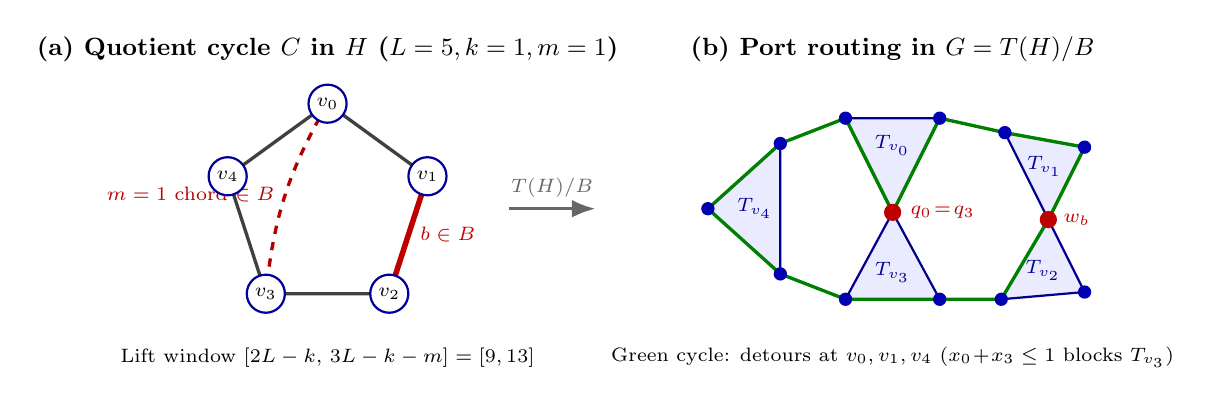
\begin{tikzpicture}[scale=0.92,
  tri/.style={fill=blue!8,draw=blue!55!black,thick},
  port/.style={circle,fill=blue!70!black,inner sep=1.7pt},
  bport/.style={circle,fill=red!75!black,inner sep=2.2pt},
  ext/.style={thick,black!75},
  det/.style={very thick,green!50!black},
  bch/.style={very thick,red!70!black,dashed}]
  % Left: quotient cycle C in H with 1 bowtie edge on C and 1 internal chordal bowtie
  \begin{scope}[xshift=-4.6cm]
    \node[font=\small\bfseries] at (0,2.2) {(a) Quotient cycle $C$ in $H$ ($L=5, k=1, m=1$)};
    \foreach \i/\ang/\lbl in {0/90/$v_0$,1/18/$v_1$,2/-54/$v_2$,3/-126/$v_3$,4/162/$v_4$} {
      \coordinate (H\i) at (\ang:1.45);
    }
    \draw[ext,very thick] (H0)--(H1) (H2)--(H3) (H3)--(H4) (H4)--(H0);
    \draw[red!75!black,line width=2pt] (H1)--(H2) node[midway,right,font=\scriptsize] {$b \in B$};
    \draw[bch] (H0) to[bend right=12] node[midway,left,font=\scriptsize,text=red!70!black] {$m=1$ chord $\in B$} (H3);
    \foreach \i/\ang/\lbl in {0/90/$v_0$,1/18/$v_1$,2/-54/$v_2$,3/-126/$v_3$,4/162/$v_4$} {
      \node[circle,draw=blue!60!black,fill=white,thick,inner sep=1.8pt,font=\scriptsize] at (H\i) {\lbl};
    }
    \node[font=\scriptsize,align=center] at (0,-2.05) {Lift window $[2L-k,\,3L-k-m] = [9, 13]$};
  \end{scope}

  % Arrow
  \draw[-{Latex[length=3mm]},very thick,black!60] (-2.1,0) -- (-0.9,0) node[midway,above,font=\scriptsize] {$T(H)/B$};

  % Right: expanded triangles showing detours, contracted bowtie, and shared chordal bowtie q0 = q3
  \begin{scope}[xshift=3.2cm]
    \node[font=\small\bfseries] at (0,2.2) {(b) Port routing in $G = T(H)/B$};
    % T0 (top): p0-, p0+, q0 (shared with q3 at center!)
    \coordinate (q03) at (0,-0.05);
    \coordinate (p0m) at (-0.65,1.25);
    \coordinate (p0p) at (0.65,1.25);
    \draw[tri] (p0m)--(p0p)--(q03)--cycle;
    \node[font=\scriptsize,blue!60!black] at (0,0.88) {$T_{v_0}$};
    % T1 (right-top) and T2 (right-bot) share bowtie w12
    \coordinate (w12) at (2.15,-0.15);
    \coordinate (p1m) at (1.55,1.05);
    \coordinate (q1)  at (2.65,0.85);
    \draw[tri] (p1m)--(w12)--(q1)--cycle;
    \node[font=\scriptsize,blue!60!black] at (2.10,0.58) {$T_{v_1}$};
    \coordinate (p2p) at (1.50,-1.25);
    \coordinate (q2)  at (2.65,-1.15);
    \draw[tri] (w12)--(p2p)--(q2)--cycle;
    \node[font=\scriptsize,blue!60!black] at (2.08,-0.85) {$T_{v_2}$};
    % T3 (bottom-center) shares q03
    \coordinate (p3m) at (0.65,-1.25);
    \coordinate (p3p) at (-0.65,-1.25);
    \draw[tri] (p3m)--(p3p)--(q03)--cycle;
    \node[font=\scriptsize,blue!60!black] at (0,-0.88) {$T_{v_3}$};
    % T4 (left)
    \coordinate (p4m) at (-1.55,-0.90);
    \coordinate (p4p) at (-1.55,0.90);
    \coordinate (q4)  at (-2.55,0.0);
    \draw[tri] (p4m)--(p4p)--(q4)--cycle;
    \node[font=\scriptsize,blue!60!black] at (-1.90,0.0) {$T_{v_4}$};

    % External edges
    \draw[ext] (p0p)--(p1m) (p2p)--(p3m) (p3p)--(p4m) (p4p)--(p0m);
    % Highlighted lifted cycle: detour at T0 (via q03), T1 (via q1), T4 (via q4); direct at T2, T3
    \draw[det] (p0m)--(q03)--(p0p)--(p1m)--(q1)--(w12)--(p2p)--(p3m)--(p3p)--(p4m)--(q4)--(p4p)--(p0m);

    % Ports
    \foreach \pt in {p0m,p0p,p1m,q1,p2p,q2,p3m,p3p,p4m,p4p,q4} {
      \node[port] at (\pt) {};
    }
    \node[bport] at (w12) {};
    \node[bport] at (q03) {};
    \node[font=\scriptsize,right=2pt,text=red!75!black] at (w12) {$w_b$};
    \node[font=\scriptsize,right=3pt,text=red!75!black] at (q03) {$q_0\!=\!q_3$};
    \node[font=\scriptsize,align=center] at (0,-2.05) {Green cycle: detours at $v_0,v_1,v_4$ ($x_0\!+\!x_3 \le 1$ blocks $T_{v_3}$)};
  \end{scope}
\end{tikzpicture}
\caption{Triangle-bowtie expansion $G = T(H)/B$ and exact lift-window routing $[2L-k, 3L-k-m]$ (Lemma~\ref{lem:lift}). Each bowtie on $C$ reduces base length by $1$ ($w_b$), and each internal chordal bowtie identifies $q_i = q_j$, allowing at most one of $T_{v_i}, T_{v_j}$ to detour.}\label{fig:lift}
\end{figure}

\subsection{R5 Dual-Crossing Sturmian Lower Bound, Bipartite-Quotient Bound, and Matching-Complement Closure}\label{subsec:r5}

We next derive from first principles the attachment lower bounds on any cycle $C$ of a simple cubic graph $H$ whose triangle replacement $G = T(H)$ avoids all dyadic cycles---equivalently, every simple cycle length of $H$ lies in $\FEG$ (giving Theorems~\ref{thm:main3}(c)--(d) and supplying the lower bounds for Theorems~\ref{thm:main2} and~\ref{thm:main3}(a)--(b)).

\begin{lemma}[Short-Chord Packing, R5 Dual-Crossing Sturmian Bound, and Bipartite-Quotient Bound]\label{lem:r5}
Let $H$ be a simple cubic graph whose triangle replacement $G = T(H)$ avoids all dyadic cycles, and let $C = (v_0, v_1, \dots, v_{y-1})$ be any simple cycle of $H$ of length $y \in \FEG$, with $M = 2^m$ ($m \ge 2$) satisfying $y = M + \delta$ and $1 \le \delta \le \lfloor M/3 \rfloor$. Let $\Vatt(C) \subseteq V(C)$ denote the set of vertices whose unique non-$C$ edge leaves $V(C)$ (bridge/attachment vertices).
\begin{enumerate}[label=(\roman*),leftmargin=2.2em]
  \item \textbf{Small Blocks ($M \in \{4, 8\}$):} $C$ has no chords at all, so $|\Vatt(C)| = y$.
  \item \textbf{General Cubic Quotient ($M \ge 16$):} Define the four-regime Sturmian template $(\alpha_R, k_R)$ by
  \[
    (\alpha_R, k_R) \;=\;
    \begin{cases}
      (3, 7)  & \text{if } 5\delta \le M + 4,\\
      (1, 3)  & \text{if } 5\delta > M + 4 \text{ and } 4\delta \le M + 2,\\
      (3, 11) & \text{if } 4\delta > M + 2 \text{ and } 31\delta \le 10M,\\
      (6, 23) & \text{if } 31\delta > 10M.
    \end{cases}
  \]
  Then
  \begin{equation}\label{eq:r5-attach}
    |\Vatt(C)| \;\ge\; y - \left\lfloor \frac{9(\delta - 1)}{4} \right\rfloor - \left\lfloor \frac{\alpha_R y}{k_R} \right\rfloor \;>\; \frac{3}{17}\, y.
  \end{equation}
  In particular, $|\Vatt(C)| > \frac{3}{17}|V(C)|$ for \emph{every} simple cycle $C \subset H$, and hence $c(H) < \frac{17}{18}|V(H)|$ and $c(G) < \frac{17}{18}|V(G)|$.
  \item \textbf{Bipartite Quotient $H$ ($M \ge 16$):} If $H$ is \emph{bipartite} (so $y$ and $\delta \ge 2$ are even), then
  \begin{equation}\label{eq:r11-bip}
    |\Vatt(C)| \;\ge\; y - \left\lfloor \frac{17(\delta - 2)}{8} \right\rfloor - \left\lfloor \frac{\alpha_R y}{k_R} \right\rfloor \;>\; \frac{1}{5}\, y,
  \end{equation}
  and hence $c(H) < \frac{15}{16}|V(H)|$ and $c(G) < \frac{15}{16}|V(G)|$.
\end{enumerate}
\end{lemma}

\begin{proof}
Because $H$ is simple cubic and $G = T(H)$ is dyadic-cycle-free, Lemma~\ref{lem:lift}(iii) ensures that every simple cycle of $H$ has length in $\FEG$. Partition $V(C) = \Vatt(C) \sqcup V_S(C) \sqcup V_L(C)$ according to the cyclic span $s \in [2, \lfloor y/2 \rfloor]$ of each chord $e = v_i v_{i+s}$ of $C$. Any chord of span $s$ yields two simple $1$-chord cycles of lengths $s + 1$ and $y - s + 1$, both in $\FEG$. Set $h := \lfloor 2M/3 \rfloor$.

(i) For $M \in \{4, 8\}$, we have $y \in \{5, 9, 10\}$; for every $2 \le s \le \lfloor y/2 \rfloor$, at least one of $s + 1, y - s + 1$ lies outside $\FEG$ (e.g., for $y = 10$, $s \in \{2, 3, 4, 5\}$ yields $s + 1 \in \{3, 4, 5, 6\}$ and $y - s + 1 \in \{9, 8, 7, 6\}$, never both in $\{5, 9, 10\}$). Hence $V_S(C) = V_L(C) = \emptyset$ and $|\Vatt(C)| = y$.

(ii) Now let $M \ge 16$. Since $y - s + 1 \in \FEG$ avoids the dyadic gap $(h, M]$, every chord of $C$ satisfies either:
\begin{itemize}[leftmargin=1.6em]
  \item \emph{Type~S (short chord):} $y - s + 1 > M$, i.e., $s \le \delta$ (and $s \ge 4$ since $s + 1 \in \FEG$ and $s \ge 2$ gives $s + 1 \ge 5$, so $s \ge 4$); or
  \item \emph{Type~L (long chord):} $y - s + 1 \le h$ and $s + 1 > M/2$, i.e., $s \in [s_{\min}, s_{\max}]$ where
  \[
    s_{\min} := \max(M/2,\, y - h + 1), \qquad s_{\max} := \min(h - 1,\, M/2 + \delta), \qquad W := s_{\max} - s_{\min}.
  \]
\end{itemize}
We bound $|V_S(C)|$ and $|V_L(C)|$ separately.

\medskip
\noindent\textbf{Step 1: Short-chord packing ($|V_S(C)| \le \lfloor 9(\delta - 1)/4 \rfloor$).}
Every Type~S chord $e = \{v_i, v_{i+s}\}$ spans a short arc $A(e) = [i, i + s]$ of $s \le \delta \le \lfloor M/3 \rfloor$ edges on $C$ and has \emph{detour gain} $g(e) := s - 1 \ge 3$ (replacing the arc $A(e)$ by the chord $e$ shortens $C$ by $g(e)$ edges). Two Type~S chords $e_1, e_2$ with disjoint arcs $A(e_1) \cap A(e_2) = \emptyset$ can be rerouted simultaneously to shorten $C$ by $g(e_1) + g(e_2)$; more generally, any collection of pairwise arc-disjoint Type~S chords with total gain $G_{\mathrm{tot}}$ yields a simple cycle of length $y - G_{\mathrm{tot}}$. Crucially, any single chord has gain $g(e) \le \delta - 1 < M - h$ (since $\delta \le M/3$ and $M - h = \lceil M/3 \rceil$), so adding disjoint Type~S chords one by one \emph{cannot jump over the forbidden gap $(h, M]$}: if a disjoint family ever achieved total gain $\ge \delta$, some prefix would achieve gain in $[\delta, \delta + \delta - 2] \subset [\delta, y - h - 1]$ and produce a cycle of length in $(h, M] \not\subset \FEG$! Therefore every arc-disjoint collection of Type~S chords has total gain at most $\delta - 1$.

Take the union $U_S := \bigcup_{e \in E_S} A(e) \subseteq C$ of the short arcs of all Type~S chords. Its connected components are either all of $C$ or vertex-disjoint paths $I_1, \dots, I_r$ on $C$ covering $V_S(C)$. For any component $I$ with $e_I$ edges ($|V(I)| = e_I + 1$ if $I$ is a path), choose a minimal subcollection of Type~S chords covering $I$; ordering them by left endpoint gives a chain $c_1, c_2, \dots, c_q$ where only consecutive chords overlap (if $c_j$ were covered by $c_{j-1} \cup c_{j+1}$ it could be dropped). Thus the even-indexed chords are pairwise arc-disjoint, and the odd-indexed chords are pairwise arc-disjoint (with at most one wraparound overlap if $U_S = C$, dropping one chord). Notice further that two crossing Type~S chords $[0, a]$ and $[c, c + b]$ ($0 < c < a < c + b$) form a simple cycle of length $2c + b - a + 2 \in \FEG$ (in particular, two span-$4$ chords cannot cross since $2c + 2 \in \{4, 6, 8\} \notin \FEG$). For a path component $I$ of $e_I$ edges:
\begin{itemize}[leftmargin=1.6em]
  \item Because consecutive chords $c_j, c_{j+1}$ in the minimal cover overlap by at least $1$ edge ($q - 1$ overlaps in total), the sum of their spans satisfies $\sum_{j=1}^q s(c_j) \ge e_I + (q - 1)$, so $\sum_{j=1}^q g(c_j) = \sum_{j=1}^q (s(c_j) - 1) \ge e_I - 1$. Partitioning into odd-indexed and even-indexed chords yields two arc-disjoint families, the heavier of which has gain at least $\lceil (e_I - 1)/2 \rceil$. For every $e_I \ge 16$, $\lceil (e_I - 1)/2 \rceil \ge \frac{4}{9}(e_I + 1)$ directly (sharp at $e_I = 17$, $[0, 9] \cup [8, 17]$, ratio $8/18 = 4/9$). (If $U_S = C$, dropping one chord leaves an even alternating cover with arc-disjoint gain $\ge \frac{1}{2}(y - 1 - \delta) \ge \frac{M - 1}{2} > \delta - 1$, impossible.)
  \item For $4 \le e_I \le 15$, the only permissible Type~S spans ($s \le e_I$ with $s + 1 \in \FEG$) are $s \in \{4, 8, 9\}$. Enumerating all endpoint-ordered minimal covers $c_1, \dots, c_q$ of $[0, e_I]$ with pairwise distinct endpoints (cubic graph condition: each start lies strictly inside the preceding chord and strictly after the penultimate end) and consecutive crossing lengths $2(l_{j+1} - l_j) + s_{j+1} - s_j + 2 \in \FEG$ yields exactly $26$ surviving chains across $4 \le e_I \le 15$ (with counts $1,0,0,0,1,1,6,1,4,3,6,3$ for $e_I = 4, \dots, 15$, and the same $26$ chains even if touching nonconsecutive endpoints are allowed; verified exhaustively in \texttt{verify\_clawfree\_eg.py}). For every surviving chain, the heavier alternating disjoint family already satisfies $9\,\mathrm{gain} \ge 4(e_I + 1)$ (for instance, the $4$-chord chain $[0, 4], [1, 10], [5, 13], [11, 15]$ at $e_I = 15$ has alternating family $[1, 10], [11, 15]$ of gain $8 + 3 = 11 > \frac{4}{9}\cdot 16$, and no two span-$4$ chords can cross, while two span-$8$ chords covering $[0, 15]$ force crossing length $16 \notin \FEG$).
\end{itemize}
Thus every component $I$ satisfies $\mathrm{gain}(I) \ge \frac{4}{9}|V(I)|$. Summing over all components gives
\[
  \frac{4}{9}|V_S(C)| \;\le\; \sum_{j=1}^r \mathrm{gain}(I_j) \;\le\; \delta - 1 \;\implies\; |V_S(C)| \;\le\; \left\lfloor \frac{9(\delta - 1)}{4} \right\rfloor.
\]

\medskip
\noindent\textbf{Step 2: Long-chord dual-crossing exclusion and Sturmian circulant averaging ($|V_L(C)| \le \lfloor \alpha_R y / k_R \rfloor$).}
If $s_{\min} > s_{\max}$, there are no Type~L chords ($|V_L(C)| = 0$). Otherwise let $W = s_{\max} - s_{\min} \ge 0$, and consider any two distinct Type~L chords $e_1 = v_i v_{i + s_1}$ and $e_2 = v_{i + d} v_{i + d + s_2}$ ($s_1, s_2 \in [s_{\min}, s_{\max}]$) whose starting endpoints lie at clockwise distance $d$ on $C$ with $W < d < s_{\min}$ and $d + s_{\max} < y$. Because $d < s_{\min} \le s_1$ and $d + s_2 > s_1$ (since $d > W \ge s_1 - s_2$) and $d + s_2 < y$, the two chords $e_1, e_2$ \emph{cross} in cyclic order $i < i + d < i + s_1 < i + d + s_2 < i + y$. Crossing chords form two simple $2$-chord cycles on $C$:
\begin{align*}
  L^{(1)} &\;=\; d + (d + s_2 - s_1) + 2 \;=\; 2d + (s_2 - s_1) + 2,\\
  L^{(2)} &\;=\; (s_1 - d) + (y - d - s_2) + 2 \;=\; y - 2d + (s_1 - s_2) + 2.
\end{align*}
Because $|s_1 - s_2| \le W$, we have $L^{(1)} \in [2d - W + 2,\, 2d + W + 2]$ and $L^{(2)} \in [y - 2d - W + 2,\, y - 2d + W + 2]$. Therefore, if $d$ satisfies the \emph{dual-forbidden condition} (\texttt{InR5DualForb}):
\begin{equation}\label{eq:dual-forb}
  \bigl(h < 2d - W + 2 \text{ and } 2d + W + 2 \le M\bigr) \quad\text{or}\quad
  \bigl(h < y - 2d - W + 2 \text{ and } y - 2d + W + 2 \le M\bigr),
\end{equation}
then at least one of $L^{(1)}, L^{(2)}$ lies in $(h, M] \not\subset \FEG$! Hence NO two vertices of $V_L(C)$ can lie at circular distance $d$ on $C$ whenever $d$ satisfies~\eqref{eq:dual-forb}.

Now let $(k_R, S_R, \alpha_R)$ be one of the four Sturmian circulant templates:
$(7, \{1\}, 3)$, $(3, \{1\}, 1)$, $(11, \{2, 4\}, 3)$, or $(23, \{3, 4, 5, 6, 7, 8\}, 6)$.
For any $u \in \mathbb{Z}_y$, form the $k_R$-element Sturmian projection $P_u := \bigl\{ \lfloor (u + j y)/k_R \rfloor \bmod y : j \in \mathbb{Z}_{k_R} \bigr\}$. For any step $s \in S_R$, the cyclic distance on $C$ between the $j$-th and $(j+s)$-th vertices of $P_u$ is always either $\lfloor s y / k_R \rfloor$ or $\lceil s y / k_R \rceil$. If both $\lfloor s y / k_R \rfloor$ and $\lceil s y / k_R \rceil$ satisfy~\eqref{eq:dual-forb} for every $s \in S_R$, then $P_u \cap V_L(C)$ pulls back to an independent set in the circulant graph $\operatorname{Circ}(k_R, S_R)$, so $|P_u \cap V_L(C)| \le \alpha(\operatorname{Circ}(k_R, S_R)) = \alpha_R$ (kernel-proved in \texttt{indep\_circulant\_7\_1}, \texttt{indep\_circulant\_3\_1}, \texttt{indep\_circulant\_11\_24}, \texttt{indep\_circulant\_23\_3to8}). Averaging over all $u \in \mathbb{Z}_y$---each vertex of $C$ appears in exactly $k_R$ sets $P_u$---yields $k_R |V_L(C)| \le \alpha_R y$, hence $|V_L(C)| \le \lfloor \alpha_R y / k_R \rfloor$.

The verification that both $\lfloor s y / k_R \rfloor$ and $\lceil s y / k_R \rceil$ satisfy~\eqref{eq:dual-forb} in the four respective regimes of $(\alpha_R, k_R)$ is linear arithmetic for all $M \ge 64$ (kernel-proved in \texttt{r5\_sturmian\_steps\_in\_dual\_forb\_ge64}) and exhaustively checked for $M \in \{16, 32\}$ (and up to $2^{18}$ in \texttt{verify\_clawfree\_eg.py}, $174{,}750$ pairs; note at $y = 18$, $M = 16$, the sole long span is $s = 9$, and for any two distinct long chords at circular distance $1 \le d \le 8$, at least one of the two crossing lengths $2d + 2$ and $20 - 2d$ lies outside $\FEG$: at both $d = 1$ and $d = 8$ the crossing lengths are $\{4, 18\}$ with $4 \notin \FEG$, while for $2 \le d \le 7$ at least one lands in $(10, 16] \not\subset \FEG$, leaving at most one antipodal long chord and hence $|V_L| \le 2 \le \lfloor 3 \cdot 18 / 7 \rfloor$). Combining Steps 1 and 2 gives~\eqref{eq:r5-attach}, and kernel-checked linear arithmetic (\texttt{r5\_attachment\_lower\_gt\_3\_17}) proves $17 |\Vatt(C)| > 3 y$ across all four regimes.

Finally, since $H$ is cubic, every vertex of $H - V(C)$ is incident to at most $3$ edges entering $C$, so $|\Vatt(C)| \le 3(|V(H)| - |V(C)|)$. Combined with $17 |\Vatt(C)| > 3 |V(C)|$, this gives $18 |V(C)| < 17 |V(H)|$ (\texttt{r5\_circumference\_17\_18}). Taking $C$ to be a longest cycle of $H$ and applying the two-sided circumference transfer $c(G) = 3 c(H)$ of Lemma~\ref{lem:lift}(ii) yields $c(G) = 3 c(H) < \frac{17}{18}(3|V(H)|) = \frac{17}{18}|V(G)|$.

(iii) When $H$ is bipartite, every simple cycle has even length, so $y = M + \delta$ is even ($\delta \ge 2$) and every Type~S chord has \emph{odd} span $s \ge 9$ (even gain $s - 1 \ge 8$, since $s + 1 \in \FEG$ is even $\implies s + 1 \ge 10$). Consider any minimal cover $c_1, \dots, c_q$ of a path component $I = [0, e_I]$ of $U_S$:
\begin{itemize}[leftmargin=1.6em]
  \item $q = 1$: gain is $e_I - 1 \ge \frac{4}{5}(e_I + 1) > \frac{8}{17}(e_I + 1)$ (as $e_I \ge 9$).
  \item $q = 2$ ($c_1 = [0, a]$, $c_2 = [b, e_I]$ with $0 < b < a < e_I$): if $e_I \le 16$, each individual chord already has even gain $g_i \ge 8$, giving $17 g_i \ge 136 = 8(16 + 1) \ge 8(e_I + 1)$ directly (e.g., at $M = 64, y = 74$, $[0, 9] \cup [4, 13]$ has $e_I = 13$ and individual gain $8 > \frac{8}{17}\cdot 14$). If $e_I \ge 17$, besides $g_1 = a - 1$ and $g_2 = e_I - b - 1$, the single crossing bypass $0 \to a \to a - 1 \to \dots \to b \to e_I$ shortens $C$ by $g_3 := e_I - (a - b + 2) = g_1 + g_2 - 2(a - b)$. Since $g_1 + g_2 + g_3 = 2 e_I - 4$, we have $\max(g_1, g_2, g_3) \ge \frac{2 e_I - 4}{3} > \frac{8}{17}(e_I + 1)$ (as $34 e_I - 68 > 24 e_I + 24 \iff 10 e_I > 92$, holding for all $e_I \ge 17$). Moreover, this crossing bypass can never jump over the forbidden gap $(h, M]$: if the running disjoint gain $G$ before $I$ satisfies $G \le \delta - 2$ and both single bypasses stay safe ($G + g_1, G + g_2 \le \delta - 2$, else $g_1$ or $g_2 \le \delta - 2 < M - h$ already lands in $(h, M]$), then $G + g_3 < (G + g_1) + g_2 \le 2(\delta - 2) < \delta + M - h$, so $G + g_3$ cannot skip $(h, M]$.
  \item $q \ge 3$: the odd-indexed and even-indexed families are arc-disjoint with even gains $O_{\mathrm{sum}}, E_{\mathrm{sum}}$ summing to $\ge e_I - 1$. Because $q \ge 3$, the odd-indexed family contains at least two chords ($c_1, c_3$), each of even gain $\ge 8$, so $\max(O_{\mathrm{sum}}, E_{\mathrm{sum}}) \ge O_{\mathrm{sum}} \ge 16 \ge \frac{8}{17}(e_I + 1)$ for all $e_I \le 33$ (sharp at $e_I = 33$, $16/34 = 8/17$). For $e_I \ge 34$, since both $O_{\mathrm{sum}}$ and $E_{\mathrm{sum}}$ are even and sum to $\ge e_I - 1$, we have $\max(O_{\mathrm{sum}}, E_{\mathrm{sum}}) \ge 2\lceil (e_I - 1)/4 \rceil \ge \frac{e_I - 1}{2} > \frac{8}{17}(e_I + 1)$ (as $17(e_I - 1) > 16(e_I + 1) \iff e_I > 33$).
\end{itemize}
Since every total gain is even and must stay $\le \delta - 2$, summing over components gives $\frac{8}{17}|V_S(C)| \le \delta - 2$, i.e., $|V_S(C)| \le \lfloor 17(\delta - 2)/8 \rfloor$. Substituting this into the same four Sturmian regimes yields~\eqref{eq:r11-bip} (\texttt{r11\_bipartite\_attachment\_lower\_gt\_1\_5}), and $5 |\Vatt(C)| > |V(C)|$ together with $|\Vatt(C)| \le 3(|V(H)| - |V(C)|)$ yields $16 c(H) < 15 |V(H)|$ and $16 c(G) < 15 |V(G)|$ (\texttt{r11\_bipartite\_circumference\_15\_16}).
\end{proof}

\begin{proof}[Proof of Theorem~\ref{thm:main3}(d) (Matching-Complement Closure)]
Suppose for contradiction that $G = T(H)$ avoids all dyadic cycles and $H$ contains a simple cycle $C$ of length $L \in \FEG$ with $\Delta(H - V(C)) \le 1$. Every component of $H - V(C)$ is either $K_1$ (a \emph{claw} $x$ with $3$ distinct attachments on $C$, forming three length-$2$ ears) or $K_2$ (an edge $xy$ with $4$ distinct attachments $\{x_1, x_2, y_1, y_2\} \subset V(C)$---distinct because $H$ is simple and $3 \notin \FEG$ makes $H$ triangle-free---forming two length-$2$ ears $x_1 x x_2, y_1 y y_2$ and four length-$3$ ears $x_i x y y_j$). Because $H$ is cubic, all chords of $C$, $K_1$-components, and $K_2$-components have pairwise disjoint attachment sets partitioning $V(C)$.

\medskip
\noindent\textbf{Step 1: Base exclusion ($L \in \{5, 9, 10\}$) and direct $M = 16$ $K_2$-exclusion.}
For $L \in \{5, 9, 10\}$ ($M \in \{4, 8\}$), no valid chord ($s + 1, L - s + 1 \in \FEG$), $K_1$ claw ($s_i \ge 3$ forces $s_1 + s_2 + s_3 \ge 9$, ruling out $L = 5$, while $(3, 3, 3)$ at $L = 9$ gives $8 \notin \FEG$ and $(3, 3, 4)$ at $L = 10$ gives $6 \notin \FEG$), or $K_2$ component exists (uncrossed Order~A gaps $g_1, g_3 \ge 3$ and $g_2, g_4 \ge 2$ sum to $\ge 10$, with $(3,2,3,2)$ giving diagonal $3+2+3 = 8 \notin \FEG$; crossed Order~B diagonals satisfy $g_1 + g_2, g_3 + g_4 \ge 7$, forcing $L \ge 14$). Thus $L = M + \delta$ with $M = 2^m \ge 16$, $1 \le \delta \le \lfloor M/3 \rfloor$, and $h := \lfloor 2M/3 \rfloor$.

For $M = 16$ ($L \in \{17, 18, 19, 20, 21\}$), exhaustive $6$-pair attachment testing over all $4$-tuples of clockwise gaps $g_1 + g_2 + g_3 + g_4 = L$ in both Order~A and Order~B (verified in \texttt{verify\_clawfree\_eg.py}) confirms that \emph{zero valid $K_2$-components exist} at $M = 16$. Hence at $M = 16$ every object on $C$ is a chord ($\ell = 1$) or a $K_1$ claw ($\ell = 2$).

\medskip
\noindent\textbf{Step 2: Exact three-band ear classification.}
Consider any length-$\ell$ ear of cyclic span $s \in [1, L - 1]$ with both $1$-ear cycle lengths $s + \ell$ and $L - s + \ell$ in $\FEG$, where either $M \ge 32$ and $\ell \in \{1, 2, 3\}$, or $M = 16$ and $\ell \in \{1, 2\}$. We claim that $s$ lies in one of three disjoint bands:
\begin{itemize}[leftmargin=1.6em]
  \item \textbf{Short $S_\ell$:} $s \le \min(\delta + \ell - 1,\, \lfloor M/3 \rfloor - \ell)$;
  \item \textbf{Long $L_\ell$:} $s + \ell, L - s + \ell \in (M/2, h]$, i.e., $s \in [s_{\min}^{(\ell)}, s_{\max}^{(\ell)}]$ where $s_{\min}^{(\ell)} = \max(M/2 + 1 - \ell,\, L - h + \ell)$ and $s_{\max}^{(\ell)} = \min(h - \ell,\, M/2 + \delta - 1 + \ell)$; by \texttt{matching\_complement\_ell\_cancellation} ($\ell \in \{1, 2, 3, 4\}$), whenever $s_{\min}^{(\ell)} \le s_{\max}^{(\ell)}$, $\ell$ cancels identically to yield
  \[
    s_{\min}^{(\ell)} \;\ge\; b_0 := \frac{5M + 6\delta + 8}{12}, \qquad L - s_{\max}^{(\ell)} \;\ge\; b_0, \qquad s_{\max}^{(\ell)} - s_{\min}^{(\ell)} \;\le\; w_0 := \frac{M - 8}{6};
  \]
  \item \textbf{Co-short $\bar{S}_\ell$:} $L - s \in S_\ell$ (so $s \ge M - \ell + 1$).
\end{itemize}
Indeed, neither $s + \ell$ nor $L - s + \ell$ can lie in the forbidden gap $(h, M]$. If $L - s + \ell \ge M + 1$, then $s \le \delta + \ell - 1$, so $s + \ell \le \delta + 2\ell - 1 \le \lfloor M/3 \rfloor + 2\ell - 1$. For $M \ge 32$ and $\ell \in \{1, 2, 3\}$, $\lfloor M/3 \rfloor + 5 \le M/2$ (equality fails even at $M = 32$: $10 + 5 = 15 < 16$); for $M = 16$ and $\ell \in \{1, 2\}$, $\lfloor 16/3 \rfloor + 3 = 8 = M/2$. Since $(\lfloor M/3 \rfloor, M/2]$ is the dyadic gap disjoint from $\FEG$, this forces $s + \ell \le \lfloor M/3 \rfloor$, i.e., $s \in S_\ell$. Symmetrically, $s + \ell \ge M + 1$ forces $s \in \bar{S}_\ell$. (For completeness, the only unoriented exceptions across all $M \ge 16$ and $\ell \in \{1, 2, 3\}$ are $(L, \ell, s) \in \{(20, 3, 6), (21, 3, 6), (21, 3, 7)\}$ at $M = 16, \ell = 3$, already ruled out by Step~1.) Otherwise both $s + \ell \le h$ and $L - s + \ell \le h$; since $\lfloor M/3 \rfloor + h = M - 1 < M + \delta + 2\ell = (s + \ell) + (L - s + \ell)$, neither can lie at or below $\lfloor M/3 \rfloor$ (nor in $(\lfloor M/3 \rfloor, M/2]$), so both lie in $(M/2, h]$, i.e., $s \in L_\ell$.

\medskip
\noindent\textbf{Step 3: Complete $K_1$ and $K_2$ dichotomies (zero mixed case).}
\begin{enumerate}[label=(\alph*),leftmargin=2em]
  \item \emph{$K_1$ claw dichotomy (all $M \ge 16$):} Let $s_1 \le s_2 \le s_3$ ($\sum s_i = L$) be the three clockwise gaps of a $K_1$ claw (all $\ell = 2$). Since $s_i + 2 \in \FEG$, we have $s_i \ge 3$. Because $s_1 \le L/3$, $L - s_1 + 2 \ge \frac{2}{3}L + 2 > h$, forcing $s_1 \in S_2$ ($s_1 \le \delta + 1$). Since $s_2 \le L/2 < M - 1$, $s_2 \notin \bar{S}_2$, so $s_2 \in S_2 \sqcup L_2$.
  \begin{itemize}[leftmargin=1.4em]
    \item If $s_2 \in S_2$ ($s_2 \le \delta + 1$), then $a := s_1 + s_2$ cannot exceed $\delta + 1$: otherwise $s_3 + 2 = L - a + 2 \le M$ while $s_3 + 2 \ge M + \delta - 2(\delta + 1) + 2 = M - \delta \ge \lceil 2M/3 \rceil > h$, placing $s_3 + 2 \in (h, M] \not\subset \FEG$! Hence $a \le \delta + 1$ (\emph{Pure Type~S $K_1$}), with outer length-$2$ ear of detour gain $a - 2$. Checking $s_1 + 2, s_2 + 2, s_1 + s_2 + 2 \in \FEG$ forces $s_1, s_2 \in \{3, 7, 8, \dots\}$ and eliminates $(3, 3), (3, 7), (3, 8), (7, 7)$, yielding exact minimum $a \ge 15$ (at $(7, 8)$), so the outer-ear gain satisfies both $a - 2 \ge 13$ and $a - 2 \ge \frac{13}{14}(a - 1)$ (with denominator $a - 1$, since $14(a - 2) - 13(a - 1) = a - 15 \ge 0$).
    \item If $s_2 \in L_2$, then $s_3 \ge s_2 \ge b_0$; since $s_3 \in \bar{S}_2$ would force $s_1 + s_2 \le \delta + 1 < b_0 \le s_2$ (impossible), we also have $s_3 \in L_2$ (\emph{Pure Type~L $K_1$}). Then $s_1 = L - s_2 - s_3 \le L - 2b_0 = w_0$, all three attachments have clockwise Type~L length-$2$ ears ($s_2, s_3$, and $s_1 + s_2 = L - s_3 \in L_2$), and every intra-$K_1$ span lies in $[1, w_0] \cup [b_0, L - b_0] \cup [L - w_0, L - 1]$, so \emph{zero} intra-$K_1$ spans lie in $(w_0, b_0)$.
  \end{itemize}
  \item \emph{$K_2$ dichotomy ($M \ge 32$):} Let $g_1 + g_2 + g_3 + g_4 = L$ be the four clockwise gaps of a $K_2$ component $xy$, with consecutive ear lengths $(\ell_1, \ell_2, \ell_3, \ell_4) = (2, 3, 2, 3)$ and diagonal ear lengths $\ell' = 3$ in Order~A (uncrossed $x_1, x_2, y_1, y_2$), or $(\ell_1, \ell_2, \ell_3, \ell_4) = (3, 3, 3, 3)$ and $\ell' = 2$ in Order~B (crossed $x_1, y_1, x_2, y_2$).
  \begin{itemize}[leftmargin=1.4em]
    \item \emph{Case 1 (some $g_i \in \bar{S}_{\ell_i}$):} All four attachments lie in a short arc of span $a := L - g_i \le \delta + \ell_i - 1$ (\emph{Pure Type~S $K_2$}) with outer ear length $\ell_i \in \{2, 3\}$ and gain $a - \ell_i$. Exhaustive small-span verification over all triples of inner gaps summing to $a$ (verified in \texttt{verify\_clawfree\_eg.py}) establishes the exact minima with respect to denominator $a - 1$: Order~B ($\ell_i = 3$) has $a \ge 14$ (attained by $(6, 2, 6)$, gain $\ge 11$, ratio $\frac{a - 3}{a - 1} \ge \frac{11}{13}$); Order~A ($\ell_i = 3$) has $a \ge 32$ (attained by $(15, 2, 15)$, ratio $\ge \frac{29}{31}$); Order~A ($\ell_i = 2$) has $a \ge 19$ (attained by $(2, 15, 2)$, ratio $\ge \frac{17}{18}$).
    \item \emph{Case 2 (no $g_i \in \bar{S}_{\ell_i}$):} Every $g_i \in S_{\ell_i} \sqcup L_{\ell_i}$. Having $0$ gaps in $L$ is impossible: since $\sum \ell_i \in \{10, 12\}$, summing $g_i \le \delta + \ell_i - 1$ yields $M + \delta \le 4\delta + 8 \implies 3\delta \ge M - 8$, whereas summing $g_i \le \lfloor M/3 \rfloor - \ell_i$ yields $M + \delta \le \frac{4M}{3} - 10 \implies 3\delta \le M - 30$, contradiction. Having exactly $1$ gap in $L$---relabeling cyclically so $g_4 \in L_{\ell_4}$ and $g_1, g_2, g_3$ are short---is also impossible: since $g_4 + \ell_4 \le h \le \frac{2M}{3}$, we have $g_1 + g_2 + g_3 = L - g_4 \ge \frac{M}{3} + \delta + \ell_4$. For the diagonal $d_1 := g_1 + g_2$ (ear length $\ell' \in \{2, 3\}$), we have $d_1 = L - g_4 - g_3 \le M + \delta - b_0 - 2 = \frac{7M + 6\delta - 32}{12} \le \frac{9M - 32}{12} < M - 2 \le M - \ell' + 1$, ruling out $d_1 \in \bar{S}_{\ell'}$. If $d_1 \in S_{\ell'}$, then $d_1 + g_3 \le (\lfloor M/3 \rfloor - \ell') + (\delta + \ell_3 - 1) \le \frac{M}{3} + \delta + (\ell_3 - \ell' - 1) \le \frac{M}{3} + \delta < \frac{M}{3} + \delta + \ell_4$ (since in Order~A $\ell' = 3, \ell_3 \le 3$ gives $\ell_3 - \ell' - 1 \le -1 < \ell_4$, and in Order~B $\ell' = 2, \ell_3 = \ell_4 = 3$ gives $0 < 3$), contradiction! Symmetrically $d_2 := g_2 + g_3 \notin S_{\ell'} \cup \bar{S}_{\ell'}$. By Step~2, both diagonals $d_1, d_2 \in L_{\ell'}$ ($\ge b_0$), forcing $g_1 = L - g_4 - d_2 \le L - 2b_0 = w_0$ and $g_2 = d_1 - g_1 \ge b_0 - w_0 = \frac{M}{4} + \frac{\delta}{2} + 2 > \delta + 2 \ge \delta + \ell_2 - 1$ (since $\delta \le M/3 < M/2$), contradicting $g_2 \in S_{\ell_2}$! Because $3 b_0 = \frac{5M + 6\delta + 8}{4} > M + \delta = L$, \emph{exact $2$ gaps} lie in $L$ ($\ge b_0$) and the remaining two gaps sum to $\le L - 2b_0 = w_0$ (\emph{Pure Type~L $K_2$}). Every intra-$K_2$ span crossing exactly one $L$-gap has both itself and its complement $\ge b_0 > \delta + 2$, so Step~2 places it in $L_\ell$; whether the two $L$-gaps are opposite or adjacent, every one of the $4$ attachments has a clockwise Type~L ear (either a direct $L$-gap, a diagonal crossing one $L$-gap, or the complementary span $L - g_j$ of an adjacent $L$-gap), and every intra-$K_2$ span crosses $0, 1,$ or $2$ $L$-gaps (lying in $[1, w_0] \cup [b_0, L - b_0] \cup [L - w_0, L - 1]$), leaving \emph{zero} intra-$K_2$ spans in $(w_0, b_0)$.
  \end{itemize}
\end{enumerate}

\medskip
\noindent\textbf{Step 4: Exact $\frac{3}{8}$-packing on overlapping short components ($M \ge 16$).}
Every Type~S object $X$ (chord: $a \ge 4$, gain $a - 1$; $K_1$: $a \ge 15$, gain $\ge \frac{13}{14}(a - 1)$; $K_2$: $a \ge 14$, gain $\ge \frac{11}{13}(a - 1)$) spans a short arc $A(X)$ of length $a(X) \le \delta + \ell(X) - 1$ with outer-ear gain $g(X) = a(X) - \ell(X) \le \delta - 1 < M - h$ and $g(X) \ge \frac{11}{13}(a(X) - 1)$. As in Lemma~\ref{lem:r5}, no arc-disjoint collection of Type~S objects can jump over $(h, M]$, so every arc-disjoint family has total gain $\le \delta - 1$. Let $U_S := \bigcup_{X \text{ Type~S}} A(X) \subseteq C$.
\begin{itemize}[leftmargin=1.6em]
  \item If $U_S = C$, take a minimal cyclic cover $X_1, \dots, X_q$ of $C$; then $\sum_{i=1}^q (a_i - 1) \ge L$. Dropping at most one object $X_q$ ($a_q - 1 \le \delta + 1$) if $q$ is odd leaves an even alternating cover with $\sum (a_i - 1) \ge L - (\delta + 1) = M - 1$, whose heavier arc-disjoint parity achieves gain $\ge \frac{11}{26}(M - 1) > \frac{M}{3} - 1 \ge \delta - 1$ (since $33(M - 1) > 26(M - 3) \iff 7M + 45 > 0$), contradiction!
  \item Thus $U_S$ is a disjoint union of path components $I_1, \dots, I_r$ on $C$. On each component $I$ ($|V(I)| = e_I + 1$), take a minimal cover $X_1, \dots, X_q$; nonconsecutive arcs are vertex-disjoint (hence distinct objects), and $\sum_{i=1}^q (a_i - 1) \ge e_I - 1$. If $|V(I)| \ge 18$, the heavier parity achieves gain $\ge \frac{11}{26}(|V(I)| - 2) \ge \frac{3}{8}|V(I)|$ (since $88(|V(I)| - 2) \ge 78|V(I)| \iff |V(I)| \ge 18$). If $|V(I)| \le 17$: if $I$ contains any $K_2$, that single $K_2$ gains $\ge 11 > \frac{3}{8}\cdot 17$; if $I$ contains any $K_1$, that single $K_1$ gains $\ge 13 > \frac{3}{8}\cdot 17$; otherwise $I$ contains only chords, so Lemma~\ref{lem:r5} (Step~1) gives gain $\ge \frac{4}{9}|V(I)| > \frac{3}{8}|V(I)|$.
\end{itemize}
Summing over all components gives $\frac{3}{8}|V_S| \le \delta - 1$, i.e., $|V_S| \le \frac{8}{3}(\delta - 1)$, and therefore
\[
  |V_L| \;=\; L - |V_S| \;\ge\; L - \frac{8}{3}(\delta - 1) \;>\; \frac{L}{3}
\]
(since $3L - 8(\delta - 1) = 3M - 5\delta + 8 \ge M + \delta + 8 = L + 8 > L$ for $\delta \le M/3$).

\medskip
\noindent\textbf{Step 5: Exact two-regime Type~L ear-crossing contradiction.}
Fix any integer step $d \in (w_0, b_0)$ (i.e., $\frac{M - 8}{6} < d < \frac{5M + 6\delta + 8}{12}$). If two vertices $u, u + d \in V_L$, then by Step~3 they \emph{must belong to distinct objects} (no chord, $K_1$, or $K_2$ has an intra-object span in $(w_0, b_0)$). Thus their clockwise Type~L ears $P_1$ (span $s_1$, length $\ell_1 \in \{1, 2, 3\}$) and $P_2$ (span $s_2$, length $\ell_2 \in \{1, 2, 3\}$) are internally vertex-disjoint with disjoint endpoints, and strictly cross ($0 < d < b_0 \le s_1 < d + s_2 < b_0 + (L - b_0) = L$, since $s_1 - s_2 \le w_0 < d$). Routing along $P_1$, $P_2$, and the two rim arcs $[u, u + d]$ and $[u + s_1, u + d + s_2]$ yields a simple cycle in $H$ of length
\[
  C_{\mathrm{cross}} \;=\; 2d + (s_2 + \ell_2) - (s_1 - \ell_1) \;=\; 2d + (s_2 + \ell_2) + (L - s_1 + \ell_1) - L.
\]
Because $s_1 \in L_{\ell_1}$ and $s_2 \in L_{\ell_2}$, we have $M/2 + 1 \le s_2 + \ell_2 \le h$, $M/2 + 1 \le L - s_1 + \ell_1 \le h$, and also $s_2 + \ell_2 = (L + 2\ell_2) - (L - s_2 + \ell_2) \ge L - h + 2$ and $L - s_1 + \ell_1 \ge L - h + 2$. Hence $\ell_1, \ell_2$ cancel completely:
\begin{equation}\label{eq:mc-cross}
  \max\bigl(2d + 2 - \delta,\; 2d + L + 4 - 2h\bigr) \;\le\; C_{\mathrm{cross}} \;\le\; 2d + 2h - L.
\end{equation}
We split into two exhaustive regimes (independently checked in \texttt{verify\_clawfree\_eg.py} for all $16 \le M \le 2^{18}$):
\begin{itemize}[leftmargin=1.6em]
  \item \textbf{Regime 1 ($13\delta < 3M + 16$):} Here $|V_L| \ge L - \frac{8}{3}(\delta - 1) > \frac{L}{2}$ (as $3(M + \delta) > 16(\delta - 1) \iff 13\delta < 3M + 16$). Consider the integer interval $[h + \delta - 1,\, 2M + \delta - 2h]$; its width is $2M - 3h + 1 \ge 2$ (since $3 \nmid M \implies 3h \le 2M - 1$), so it contains at least one \emph{even} integer $2d$. Then $2d \ge h + \delta - 1 \ge \frac{2M - 2}{3} > \frac{M - 8}{3} = 2w_0$ and $2d \le 2M + \delta - 2h \le \frac{2M + 3\delta + 4}{3} < \frac{5M + 6\delta + 8}{6} = 2b_0$, so $d \in (w_0, b_0)$. By~\eqref{eq:mc-cross}, $C_{\mathrm{cross}} \ge 2d + 2 - \delta \ge h + 1 > h$ and $C_{\mathrm{cross}} \le 2d + 2h - L \le 2M + \delta - L = M$, placing $C_{\mathrm{cross}} \in (h, M] \not\subset \FEG$! Hence no pair $\{u, u + d\}$ lies in $V_L$; averaging over $u \in \mathbb{Z}_L$ forces $|V_L| \le L/2$, contradiction!
  \item \textbf{Regime 2 ($13\delta \ge 3M + 16$, so $\delta \ge 5$):} Take either $d \in \{\lfloor L/3 \rfloor, \lceil L/3 \rceil\}$ (so $L - 2 \le 3d \le L + 2$). Then $6d \ge 2L - 4 = 2M + 2\delta - 4 > M - 8 = 6w_0$ and $12d \le 4L + 8 = 4M + 4\delta + 8 < 5M + 6\delta + 8 = 12b_0$, so $d \in (w_0, b_0)$. Using $6h \le 4M - 2$ and $9h \le 6M - 3$, the second lower bound in~\eqref{eq:mc-cross} gives
  \[
    3\, C_{\mathrm{cross}} \;\ge\; 6d + 3L + 12 - 6h \;\ge\; 5L + 8 - 6h \;\ge\; M + 5\delta + 10 \;>\; 3h
  \]
  (indeed $5\delta - M + 11 \ge \frac{15M + 80}{13} - M + 11 = \frac{2M + 223}{13} > 0$), while the upper bound gives
  \[
    3\, C_{\mathrm{cross}} \;\le\; 6d + 6h - 3L \;\le\; 6h - L + 4 \;\le\; 3M - \delta + 2 \;<\; 3M
  \]
  (since $\delta \ge 5 > 2$). Thus $C_{\mathrm{cross}} \in (h, M] \not\subset \FEG$ for BOTH $d \in \{\lfloor L/3 \rfloor, \lceil L/3 \rceil\}$. Averaging over the cyclic triples $\{u, u + \lfloor L/3 \rfloor, u + \lfloor 2L/3 \rfloor\} \pmod L$ (whose pairwise distances lie in $\{\lfloor L/3 \rfloor, \lceil L/3 \rceil\}$) forces $|V_L| \le L/3$, contradicting $|V_L| > L/3$! \qedhere
\end{itemize}
\end{proof}

%% =============================================================================
\section{Proof of Main Theorem 1: Sub-Unit 2D Dyadic \texorpdfstring{$L_\infty$}{L-infinity}-Packing}\label{sec:packing}
%% =============================================================================

\subsection{45\texorpdfstring{$^\circ$}{deg}-Rotated Bridge Coordinates and the Exact Packing Domain}\label{subsec:bridge-encoding}

Before proving Theorem~\ref{thm:main1}, we verify why every bridge-packing application in Sections~\ref{sec:twocycle} and~\ref{sec:polyk} automatically satisfies hypotheses~(i)--(iii) of Theorem~\ref{thm:main1}.

\begin{lemma}[Bridge-Coordinate Rotation to the No-Diagonal Parity Lattice]\label{lem:bridge-encoding}
Suppose $A \subset V(C_1)$ and $B \subset V(C_2)$ are vertex-disjoint paths (or cycle arcs with no wraparound, so linear distance equals cyclic distance) indexed by integers $i \in [0, a]$ and $j \in [0, b]$. Let $E_0 \subseteq A \times B$ be a set of pairwise vertex-disjoint edges (bridges) in a simple cubic graph $H$ such that for every pair of distinct bridges $(i_1, j_1), (i_2, j_2) \in E_0$, the simple cycle formed by the two bridges and the connecting subpaths on $A$ and $B$ has length $|i_1 - i_2| + |j_1 - j_2| + 2 \in \FEG$. Map each bridge $(i, j) \in E_0$ to the $45^\circ$-rotated coordinate
\[
  (u, v) \;:=\; (i + j,\; i - j + b) \;\in\; [0, a + b] \times [0, a + b].
\]
Then the image $S := \{(u, v) : (i, j) \in E_0\}$ satisfies all three hypotheses~(i)--(iii) of Theorem~\ref{thm:main1}:
\begin{enumerate}[label=(\roman*),leftmargin=2.2em]
  \item $u + v = 2i + b \equiv b \pmod{2}$ has constant parity across $S$;
  \item $|u_1 - u_2| \neq |v_1 - v_2|$ for all distinct $(u_1, v_1), (u_2, v_2) \in S$;
  \item $\max(|u_1 - u_2|, |v_1 - v_2|) = |i_1 - i_2| + |j_1 - j_2|$, so $\max(|u_1 - u_2|, |v_1 - v_2|) + 2 \in \FEG$.
\end{enumerate}
\end{lemma}

\begin{proof}
(i) $u + v = (i + j) + (i - j + b) = 2i + b \equiv b \pmod{2}$ is independent of $(i, j)$.
(ii) Let $\Delta i := i_1 - i_2$ and $\Delta j := j_1 - j_2$. Then $u_1 - u_2 = \Delta i + \Delta j$ and $v_1 - v_2 = \Delta i - \Delta j$. Hence $|u_1 - u_2| = |v_1 - v_2|$ holds if and only if $(\Delta i + \Delta j)^2 = (\Delta i - \Delta j)^2$, i.e., $4 \Delta i \Delta j = 0$, i.e., $i_1 = i_2$ or $j_1 = j_2$. Because the bridges in $E_0$ are pairwise vertex-disjoint, distinct bridges have $i_1 \neq i_2$ and $j_1 \neq j_2$, so $|u_1 - u_2| \neq |v_1 - v_2|$ strictly!
(iii) For all real numbers $\Delta i, \Delta j$, $\max(|\Delta i + \Delta j|, |\Delta i - \Delta j|) = |\Delta i| + |\Delta j|$.
\end{proof}

\subsection{Dyadic Block Decomposition, 4-Corner Orbits, and Orbit \texorpdfstring{\texttt{1001}}{1001} H/V-Merges}\label{subsec:dyadic-decomp}

For any integers $W_1, W_2 \ge 0$, let $F(W_1, W_2)$ denote the maximum cardinality $|S|$ over all subsets $S \subset [0, W_1] \times [0, W_2]$ satisfying hypotheses~(i)--(iii) of Theorem~\ref{thm:main1}; by convention we extend $F(W_1, W_2) := 0$ whenever $W_1 < 0$ or $W_2 < 0$ (representing an empty bounding box), while $F(0, 0) = 1$. Clearly $F(W_1, W_2) = F(W_2, W_1)$ (by swapping coordinates) and $F$ is coordinatewise nondecreasing in both arguments. Moreover, shifting any nonempty valid packing $S$ so that $\min_{(u,v) \in S} u = 0$ and $\min_{(u,v) \in S} v = 0$ preserves parity, no-diagonal collisions, and $L_\infty$-distances; thus $F(W_1, W_2)$ is achieved on a tight bounding box $[0, W_1'] \times [0, W_2']$ with $W_1' \le W_1$, $W_2' \le W_2$.

\begin{lemma}[Base Table $F_{19}$ and Dyadic Gap Collapse]\label{lem:gap-collapse}
\leavevmode
\begin{enumerate}[label=(\roman*),leftmargin=2.2em]
  \item For all $0 \le W_2 \le W_1 \le 19$, the exact clique maximum $F(W_1, W_2) = F_{19}[W_1, W_2]$ ($210$ lower-triangular entries, $F_{19}[19, 19] = 8$, $F_{19}[3, 1] = 2$, $F_{19}[2, 1] = 1$) satisfies~\eqref{eq:packing-main}.
  \item For every power of two $m = 2^k \ge 32$, set
  \[
    L_m \;:=\; m - 1, \qquad U_m \;:=\; \left\lfloor \frac{2m}{3} \right\rfloor - 2, \qquad W_{\max}(m) \;:=\; \left\lfloor \frac{4m}{3} \right\rfloor - 2,
  \]
  and similarly at half-scale $m_h := m/2$: $L_h := m_h - 1$, $U_h := \lfloor 2m_h / 3 \rfloor - 2$. Then no integer $d \in (U_m, L_m)$ satisfies $d + 2 \in \FEG$ (\texttt{gap\_outside\_feg}). Consequently, whenever $W_1, W_2 \in [U_m + 1, L_m - 1]$ (or whenever $U_m < W_1 < L_m$ and $W_2 \le W_1$), every valid packing $S \subset [0, W_1] \times [0, W_2]$ has $\max(|u_1 - u_2|, |v_1 - v_2|) \le U_m$ for all $p, q \in S$, and hence fits after translation inside $[0, U_m] \times [0, \min(W_2, U_m)]$:
  \begin{equation}\label{eq:gap-collapse}
    F(W_1, W_2) \;=\; F\bigl(\min(W_1, U_m),\, \min(W_2, U_m)\bigr) \qquad \text{whenever } U_m < W_1 < L_m,\; W_2 \le W_1.
  \end{equation}
  (In particular, for $m = 32$, $U_{32} = 19$ and $L_{32} = 31$, so $[20, 30]$ collapses directly to $F_{19}$!)
\end{enumerate}
\end{lemma}

\begin{proof}
(i) For each $0 \le W_2 \le W_1 \le 19$ and parity $p \in \{0, 1\}$, \texttt{verify\_clawfree\_eg.py} (\texttt{compute\_exact\_base\_f19}) builds the exact compatibility graph on $\{(x, y) \in [0, W_1] \times [0, W_2] : x + y \equiv p \pmod 2\}$ with edges $\{p, q\}$ iff $|x_1 - x_2| \neq |y_1 - y_2|$ and $\max(|x_1 - x_2|, |y_1 - y_2|) + 2 \in \FEG$, and computes the exact clique number by exhaustive bitset branch-and-bound. Lean~4 kernel-verifies all $210$ numeric entries against~\eqref{eq:packing-main} (\texttt{f19\_packing\_bound}) and monotonicity (\texttt{f19\_monotone\_x}, \texttt{f19\_monotone\_y}).

(ii) If $U_m < d < L_m$, then $\lfloor 2m/3 \rfloor < d + 2 \le m$, which is precisely the dyadic gap between $(m/2, \lfloor 2m/3 \rfloor]$ and $(m, \lfloor 4m/3 \rfloor]$; hence $d + 2 \notin \FEG$. Thus if $W_2 \le W_1 < L_m$, every pair $p, q \in S \subset [0, W_1] \times [0, W_2]$ has $\|p - q\|_\infty \le W_1 < L_m$, forcing $\|p - q\|_\infty \le U_m$ (\texttt{square\_gap\_collapse}). Translating $S$ by $(-\min u, -\min v)$ embeds $S$ into $[0, \min(W_1, U_m)] \times [0, \min(W_2, U_m)]$.
\end{proof}

Now fix a dyadic scale $m = 2^k \ge 32$ and a rectangle $[0, W_1] \times [0, W_2]$ with $L_m \le W_1 \le W_{\max}(m)$ and $0 \le W_2 \le W_1$. Set $s_1 := W_1 - L_m \in [0, \lfloor m/3 \rfloor - 1]$, and partition the $x$-range $[0, W_1]$ into three disjoint strips:
\[
  X_0 := [0, s_1], \qquad X_1 := [s_1 + 1, L_m - 1], \qquad X_2 := [L_m, W_1].
\]
Observe the fundamental gap-separation property:
\begin{itemize}[leftmargin=1.6em]
  \item Every point in $X_0$ and every point in $X_2$ differ in $x$ by at least $L_m - s_1 > U_m$ (since $L_m - s_1 = 2m - 2 - W_1 \ge \lceil 2m/3 \rceil > U_m$).
  \item Consequently, if $p \in X_0 \times [0, W_2]$ and $q \in X_2 \times [0, W_2]$ satisfy $|y(p) - y(q)| < L_m$, then $\|p - q\|_\infty$ cannot lie in $(U_m, L_m)$, which forces $x(q) - x(p) \ge L_m$! Letting $a := \max_{p \in S_0} x(p)$ and $b := \min_{q \in S_2} x(q)$ for any two nonempty subsets $S_0 \subseteq X_0 \times I$, $S_2 \subseteq X_2 \times I$ on a common $y$-interval $I$ of height $< L_m$, we get $b - a \ge L_m$, so the horizontal widths $w(S_0) \le a$ and $w(S_2) \le W_1 - b$ satisfy the \emph{cross-strip width sum constraint}:
  \begin{equation}\label{eq:strip-sum}
    w(S_0) + w(S_2) \;\le\; a + (W_1 - b) \;\le\; W_1 - L_m \;=\; s_1.
  \end{equation}
  (If either $S_0$ or $S_2$ is empty, the remaining set still has width $\le s_1$.)
  \item Likewise, any point in $X_1$ has distance $< L_m$ to BOTH $x = 0$ and $x = W_1$. If $S$ is tight in $x$ (containing a point at $x = 0$ and a point at $x = W_1$) and restricted to $y$-height $< L_m$, then any $p \in X_1$ must stay within $U_m$ of $0$ (forcing $x(p) \le U_m$) and within $U_m$ of $W_1$ (forcing $x(p) \ge W_1 - U_m$), so the $x$-diameter of $X_1$ is at most $2 U_m - W_1 = (2 U_m - L_m) - s_1 \le \frac{m}{3} - s_1 - 3$!
\end{itemize}

\begin{figure}[t]
\centering
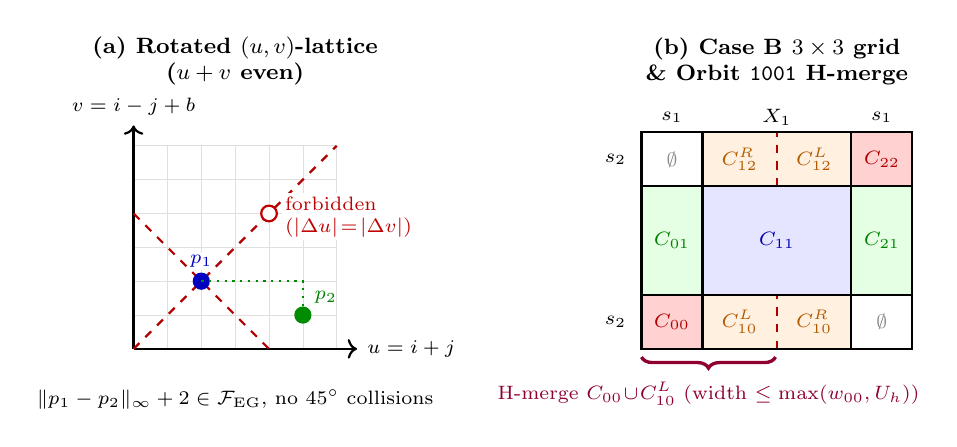
\begin{tikzpicture}[scale=0.86,
  cell/.style={draw=black!50,thin},
  corn/.style={fill=red!18,draw=red!60!black,thick},
  midc/.style={fill=blue!12,draw=blue!55!black,thick},
  edgc/.style={fill=orange!15,draw=orange!70!black}]
  % Left: 45-degree rotated parity lattice & no-diagonal
  \begin{scope}[xshift=-5.2cm,yshift=-0.2cm]
    \node[font=\footnotesize\bfseries,align=center] at (1.5,4.25) {(a) Rotated $(u,v)$-lattice\\($u+v$ even)};
    \draw[step=0.5,gray!25,very thin] (0,0) grid (3.0,3.0);
    \draw[->,thick] (0,0) -- (3.3,0) node[right,font=\scriptsize] {$u=i+j$};
    \draw[->,thick] (0,0) -- (0,3.3) node[above,font=\scriptsize] {$v=i-j+b$};
    % Diagonal forbidden lines through (1.0,1.0)
    \draw[red!70!black,dashed,thick] (0,0) -- (3.0,3.0);
    \draw[red!70!black,dashed,thick] (0,2.0) -- (2.0,0);
    \node[circle,fill=blue!75!black,inner sep=2.2pt] (P0) at (1.0,1.0) {};
    \node[font=\scriptsize,above=4pt,blue!75!black,fill=white,inner sep=0.8pt] at (P0) {$p_1$};
    \node[circle,fill=green!55!black,inner sep=2.2pt] (P1) at (2.5,0.5) {};
    \node[font=\scriptsize,above right=1pt,green!50!black] at (P1) {$p_2$};
    \draw[green!55!black,thick,dotted] (1.0,1.0)--(2.5,1.0)--(2.5,0.5);
    \node[circle,draw=red!75!black,fill=white,thick,inner sep=2pt] at (2.0,2.0) {};
    \node[font=\scriptsize,align=left,anchor=west,red!75!black,fill=white,inner sep=1.2pt] at (2.18,1.95) {forbidden\\($|\Delta u|\!=\!|\Delta v|$)};
    \node[font=\scriptsize,align=center] at (1.5,-0.75) {$\|p_1-p_2\|_\infty+2 \in \FEG$, no $45^\circ$ collisions};
  \end{scope}

  % Right: 3x3 Case B grid + Orbit 1001 H-merge
  \begin{scope}[xshift=2.3cm,yshift=-0.2cm]
    \node[font=\footnotesize\bfseries,align=center] at (2.0,4.25) {(b) Case~B $3\times 3$ grid\\\& Orbit \texttt{1001} H-merge};
    % Grid lines at 0, 0.9, 3.1, 4.0 (x) and 0, 0.8, 2.4, 3.2 (y)
    \fill[red!18] (0,0) rectangle (0.9,0.8);
    \fill[red!18] (3.1,2.4) rectangle (4.0,3.2);
    \fill[blue!10] (0.9,0.8) rectangle (3.1,2.4);
    \fill[orange!12] (0.9,0) rectangle (3.1,0.8);
    \fill[orange!12] (0.9,2.4) rectangle (3.1,3.2);
    \fill[green!10] (0,0.8) rectangle (0.9,2.4);
    \fill[green!10] (3.1,0.8) rectangle (4.0,2.4);
    % Double-gap split inside C10
    \draw[red!70!black,thick,dashed] (2.0,0) -- (2.0,0.8);
    \draw[red!70!black,thick,dashed] (2.0,2.4) -- (2.0,3.2);
    % Outer and inner grid
    \draw[thick] (0,0) rectangle (4.0,3.2);
    \draw[thick] (0.9,0)--(0.9,3.2) (3.1,0)--(3.1,3.2) (0,0.8)--(4.0,0.8) (0,2.4)--(4.0,2.4);
    % Labels
    \node[font=\scriptsize\bfseries,red!70!black] at (0.45,0.4) {$C_{00}$};
    \node[font=\scriptsize,black!45] at (3.55,0.4) {$\emptyset$};
    \node[font=\scriptsize,black!45] at (0.45,2.8) {$\emptyset$};
    \node[font=\scriptsize\bfseries,red!70!black] at (3.55,2.8) {$C_{22}$};
    \node[font=\scriptsize,blue!70!black] at (2.0,1.6) {$C_{11}$};
    \node[font=\scriptsize,orange!70!black] at (1.45,0.4) {$C_{10}^L$};
    \node[font=\scriptsize,orange!70!black] at (2.55,0.4) {$C_{10}^R$};
    \node[font=\scriptsize,orange!70!black] at (1.45,2.8) {$C_{12}^R$};
    \node[font=\scriptsize,orange!70!black] at (2.55,2.8) {$C_{12}^L$};
    \node[font=\scriptsize,green!50!black] at (0.45,1.6) {$C_{01}$};
    \node[font=\scriptsize,green!50!black] at (3.55,1.6) {$C_{21}$};
    % Brace for H-merge of C00 union C10^L
    \draw[decorate,decoration={brace,mirror,amplitude=4pt},very thick,purple!75!black] (0,-0.12) -- (1.98,-0.12)
      node[midway,below=5pt,font=\scriptsize,text=purple!75!black] {H-merge $C_{00}\!\cup\! C_{10}^L$ (width $\le \max(w_{00}, U_h)$)};
    % Axis ticks
    \node[font=\scriptsize] at (0.45,3.42) {$s_1$};
    \node[font=\scriptsize] at (2.0,3.42) {$X_1$};
    \node[font=\scriptsize] at (3.55,3.42) {$s_1$};
    \node[font=\scriptsize,left=2pt] at (0,0.4) {$s_2$};
    \node[font=\scriptsize,left=2pt] at (0,2.8) {$s_2$};
  \end{scope}
\end{tikzpicture}
\caption{2D Dyadic $L_\infty$-Packing geometry (Section~\ref{sec:packing}). (a)~$45^\circ$-rotated bridge coordinates with constant parity and forbidden $45^\circ$ diagonals. (b)~Case~B $3 \times 3$ strip partition at scale $m = 2^k$, illustrating Orbit~\texttt{1001} and the horizontal merge $C_{00} \cup C_{10}^L$ bounded by half-scale width $\max(w_{00}, U_{m/2}) \le \frac{m}{3} - 1$.}\label{fig:packing}
\end{figure}

This yields two cases for any tight valid packing $S \subset [0, W_1] \times [0, W_2]$ with $L_m \le W_1 \le W_{\max}(m)$ and $0 \le W_2 \le W_1$:

\medskip
\noindent\textbf{Case A ($W_2 < L_m$).}
Because every pair of points in $S$ has $|\Delta y| \le W_2 < L_m$, we partition $S = S_0 \sqcup S_1 \sqcup S_2$ across the three $X$-strips $X_0, X_1, X_2$ \emph{first}. By~\eqref{eq:strip-sum}, the horizontal widths of the outer strips satisfy $w(S_0) + w(S_2) \le s_1 < L_m$, and tightness of $S$ at $x = 0$ and $x = W_1$ gives $w(S_1) \le 2 U_m - W_1 < L_m$ (with $S_1 = \emptyset$ whenever $2U_m - W_1 < 0$). Now \emph{every nonempty child} $S_j$ ($j \in \{0, 1, 2\}$) has \emph{both} horizontal span $< L_m$ and vertical span $\le W_2 < L_m$; hence Lemma~\ref{lem:gap-collapse}(ii) legitimately collapses the vertical span of each child $S_j$ to $W_2' := \min(W_2, U_m)$! With the empty-child convention $F(w, h) = 0$ for $w < 0$,
\begin{equation}\label{eq:caseA-rec}
  |S| \;\le\; \max_{t_0 + t_2 \le s_1}\bigl(F(t_0, W_2') + F(t_2, W_2')\bigr) + F(2 U_m - W_1, W_2'), \qquad W_2' := \min(W_2, U_m).
\end{equation}
In particular, when $U_m < W_2 < L_m$, every child evaluates at height $W_2' = U_m$, which justifies copying the DP upper bound $U[W_1][W_2] := U[W_1][U_m]$ in Regime~2 below.

\medskip
\noindent\textbf{Case B ($L_m \le W_2 \le W_1 \le W_{\max}(m)$).}
Set $s_2 := W_2 - L_m \in [0, s_1]$ and partition $[0, W_2]$ analogously into $Y_0 = [0, s_2]$, $Y_1 = [s_2 + 1, L_m - 1]$, $Y_2 = [L_m, W_2]$. This divides $[0, W_1] \times [0, W_2]$ into nine cells $C_{ij} := S \cap (X_i \times Y_j)$ ($i, j \in \{0, 1, 2\}$; see Figure~\ref{fig:packing}(b)). Every cell has width and height $\le U_m$ (since $s_1, s_2 < \frac{m}{3} \le U_m$ and $|X_1|, |Y_1| < L_m$ collapse by~\eqref{eq:gap-collapse}). Classify $S$ by its $4$-bit corner occupancy mask $(b_{00}, b_{20}, b_{02}, b_{22}) \in \{0, 1\}^4$, where $b_{ij} = 1$ iff $C_{ij} \neq \emptyset$. Under the $4$-element reflection group $\mathbb{Z}_2 \times \mathbb{Z}_2$ acting on the horizontal and vertical axes, the $16$ corner masks partition into $7$ symmetry orbits of sizes $1 + 4 + 2 + 2 + 4 + 1 + 2 = 16$ (\texttt{corner\_orbit\_partition\_16}):
\begin{enumerate}[label=(\arabic*),leftmargin=2em]
  \item \textbf{Orbit \texttt{0000} ($\times 1$):} All four corners are empty. Since $S$ is tight on $[0, W_1] \times [0, W_2]$, the global $x$-extrema lie in $C_{01}$ and $C_{21}$ (both in $Y_1$), and the global $y$-extrema lie in $C_{10}$ and $C_{12}$ (both in $X_1$). Every point of $C_{10} \cup C_{11} \cup C_{12}$ has $|\Delta y| < L_m$ to $C_{01}$ and $C_{21}$ (since $Y_1 \subset [s_2 + 1, L_m - 1]$ is strictly within $L_m - 1$ of both $0$ and $W_2$), forcing $w(C_{10}), w(C_{11}), w(C_{12}) \le 2 U_m - W_1 =: w_{11}$. Symmetrically $h(C_{01}), h(C_{11}), h(C_{21}) \le 2 U_m - W_2 =: h_{11}$, while cross-strip separation~\eqref{eq:strip-sum} gives $h(C_{10}) + h(C_{12}) \le s_2$ and $w(C_{01}) + w(C_{21}) \le s_1$.
  \item \textbf{Orbit \texttt{1000} ($\times 4$):} Only $C_{00} \neq \emptyset$ (width $w_0 \le s_1$, height $h_0 \le s_2$). The global extrema at $x = W_1$ and $y = W_2$ lie in $C_{21}$ and $C_{12}$, giving $w(C_{11}), w(C_{10}) \le w_{11}$ and $h(C_{11}), h(C_{01}) \le h_{11}$. For $C_{12}$ (opposite $C_{00}$ in $y$), its points have $|\Delta y| \ge L_m - s_2 > U_m$ to $C_{00}$ (so no constraint from $x = 0$ if $x = 0$ is in $C_{00}$), but its distance to $C_{21}$ ($x = W_1$, $|\Delta y| < L_m$) forces $x \ge W_1 - U_m$, so $w(C_{12}) \le U_m - s_1 - 1$; symmetrically $h(C_{21}) \le U_m - s_2 - 1$. Meanwhile, comparing $C_{00} \cup C_{10}$ against $C_{12}$ yields $h(C_{10}) + h(C_{12}) \le s_2$ with $h(C_{12}) \le s_2 - h_0$, and symmetrically $w(C_{01}) + w(C_{21}) \le s_1$ with $w(C_{21}) \le s_1 - w_0$.
  \item \textbf{Orbits \texttt{1100} and \texttt{1010} ($\times 2$ each):} In \texttt{1100} ($C_{00}, C_{20} \neq \emptyset$), merge the left column $L := C_{00} \cup C_{01}$ (width $w_L$, height $\le U_m$ since $C_{02} = \emptyset$) and the right column $R := C_{20} \cup C_{21}$ (width $w_R$, height $\le U_m$). Since $L, R$ both lie in $[0, L_m - 1]$ in $y$,~\eqref{eq:strip-sum} gives $w_L + w_R \le s_1$. For $C_{10}$, its points are constrained by both $C_{00}$ and $C_{20}$ (which lie in $Y_0$, $|\Delta y| < L_m$), so $w(C_{10}) \le 2 U_m - L_m$. For $C_{12}$, its $x$-span is bounded by $\min(U_m, L_m - 2 - s_1)$ (distance to $X_0$ or $X_2$ if $C_{01}$ or $C_{21}$ has height $< L_m$; in fact $x \in [s_1 + 1, L_m - 1]$ has diameter $L_m - 2 - s_1$, and gap-collapse caps it at $U_m$). And $h(C_{10}) + h(C_{12}) \le s_2$, $C_{11} \subset [w_{11}] \times [h_{11}]$. Orbit \texttt{1010} is the coordinate swap $x \leftrightarrow y$.
  \item \textbf{Orbit \texttt{1110} ($\times 4$):} $C_{00}, C_{20}, C_{02} \neq \emptyset$ and $C_{22} = \emptyset$. Merge the right column $R := C_{20} \cup C_{21}$ (width $u_2$, height $\le U_m$) and the top row $T := C_{02} \cup C_{12}$ (height $v_2$, width $\le U_m$). Let $u_1 := w(C_{00} \cup C_{01})$ and $v_1 := h(C_{00} \cup C_{10})$; then $u_1 + u_2 \le s_1$ and $v_1 + v_2 \le s_2$ (comparing $C_{00} \cup C_{01}$ against $R$ on $[0, L_m - 1]$ in $y$, and $C_{00} \cup C_{10}$ against $T$ on $[0, L_m - 1]$ in $x$). Write the $x$-extent of $C_{00}$ as $[a_0, a_0 + w_0]$ ($w_0 \le u_1$) and its $y$-extent as $[b_0, b_0 + h_0]$ ($h_0 \le v_1$). Every point of $C_{20}$ lies in $Y_0$ ($|\Delta y| \le s_2 < L_m$) and therefore satisfies $x \ge (a_0 + w_0) + L_m$, while every point of $C_{10}$ has $x$-distance $\le U_m$ to both $a_0$ (in $C_{00}$) and $x_{\min}(C_{20}) \ge a_0 + w_0 + L_m$. Hence $x(C_{10}) \subseteq [a_0 + w_0 + L_m - U_m,\, a_0 + U_m]$, which has width at most $2 U_m - L_m - w_0$. Symmetrically $h(C_{01}) \le 2 U_m - L_m - h_0$. Thus $C_{00} \cup C_{10} \cup C_{01}$ contributes at most $F(w_0, h_0) + F(2 U_m - L_m - w_0, v_1) + F(u_1, 2 U_m - L_m - h_0)$.
  \item \textbf{Orbit \texttt{1111} ($\times 1$):} All four corners are nonempty. Set $u_B := w(C_{00}) + w(C_{20}) \le s_1$, $u_T := w(C_{02}) + w(C_{22}) \le s_1$, $v_L := h(C_{00}) + h(C_{02}) \le s_2$, $v_R := h(C_{20}) + h(C_{22}) \le s_2$. By the same gap argument between $C_{00}$ and $C_{20}$, $w(C_{10}) \le 2 U_m - L_m - u_B$ (indeed, $x_{\max}(C_{10}) \le x_{\min}(C_{00}) + U_m$ and $x_{\min}(C_{10}) \ge x_{\max}(C_{20}) - U_m$; since $x_{\max}(C_{20}) - x_{\min}(C_{00}) \ge L_m + u_B$, subtracting gives $w(C_{10}) \le 2 U_m - L_m - u_B$!). Similarly $w(C_{12}) \le 2 U_m - L_m - u_T$, $h(C_{01}) \le 2 U_m - L_m - v_L$, $h(C_{21}) \le 2 U_m - L_m - v_R$. For the four corners themselves, by $3$-factor H\"older's inequality with exponents $(1/\alpha, 1/\alpha, 1/(1 - 2\alpha))$ applied to the four terms $C (w_{ij} + 2)^\alpha (h_{ij} + 2)^\alpha$:
  \begin{align}
    \sum_{i, j \in \{0, 2\}} C (w_{ij} + 2)^\alpha (h_{ij} + 2)^\alpha
    &\;\le\; C \cdot 4^{1 - 2\alpha} \Bigl(\sum (w_{ij} + 2)\Bigr)^\alpha \Bigl(\sum (h_{ij} + 2)\Bigr)^\alpha \notag\\
    &\;=\; 4 C \left(\frac{u_B + u_T + 8}{4}\right)^\alpha \left(\frac{v_L + v_R + 8}{4}\right)^\alpha. \label{eq:1111-holder}
  \end{align}
  \item \textbf{Orbit \texttt{1001} ($\times 2$, Double-Gap \& H/V-Merge):} $C_{00}, C_{22} \neq \emptyset$ and $C_{20} = C_{02} = \emptyset$. By $180^\circ$ rotation symmetry $(x, y) \mapsto (W_1 - x, W_2 - y)$, we may assume without loss of generality that $w_0 := w(C_{00}) \le w(C_{22}) =: w_2$. Let $h_0 := h(C_{00})$ and $h_2 := h(C_{22})$. Write the horizontal extent of $C_{00}$ as $[a_0, a_0 + w_0] \subseteq [0, s_1]$, so $0 \le a_0 \le s_1 - w_0$.
  \begin{itemize}[leftmargin=1.4em]
    \item \emph{Half-scale double-gap split of $C_{10}$:} Because $C_{02} = \emptyset$, the global $x = 0$ point lies in $C_{00} \cup C_{01}$, so every point of $C_{10}$ has $x \le U_m$ (as $C_{00} \cup C_{01} \subset [0, L_m - 1]$ in $y$). Moreover, $C_{00} \cup C_{10} \subset Y_0$ has vertical height $\le s_2 < \frac{m}{3} < L_h = m/2 - 1$. Therefore, for every $p \in C_{10}$, its horizontal distances $x(p) - a_0$ and $x(p) - (a_0 + w_0)$ to the two $x$-endpoints of $C_{00}$ \emph{cannot lie in the half-scale gap $(U_h, L_h)$}! Thus $C_{10}$ partitions into a \emph{left piece} $C_{10}^L := \{p \in C_{10} : x(p) \le a_0 + U_h\}$ (lying in $[s_1 + 1, a_0 + U_h]$, so width $w_L \le a_0 + U_h - s_1 - 1$) and a \emph{right piece} $C_{10}^R := \{p \in C_{10} : x(p) \ge a_0 + L_h\}$. Every $p \in C_{10}^R$ also avoids $(U_h, L_h)$ from $a_0 + w_0$, giving either $x(p) \ge a_0 + w_0 + L_h$ (if $w_0 \le U_m - L_h$, width $\le U_m - a_0 - w_0 - L_h$) or $x(p) \le a_0 + w_0 + U_h$ (if $w_0 \ge L_h - U_h$, width $\le \min(U_m - a_0 - L_h,\, w_0 + U_h - L_h)$). Since $U_m - L_h < L_h - U_h$ (\texttt{dyadic\_subinterval\_algebra\_pow2}), these two right-piece subintervals are strictly separated by a half-scale gap and mutually exclusive! Thus $|C_{10}| \le \min\bigl(F(U_m - s_1 - 1, h_{10}),\, F(w_L, h_{10}) + F(w_R, h_{10})\bigr)$.
    \item \emph{Horizontal merge ($C_{00} \cup C_{10}^L$):} Observe that $C_{00} \cup C_{10}^L$ lies horizontally inside $[a_0, \max(a_0 + w_0, a_0 + U_h)]$, which has width at most
    \[
      w_{\mathrm{mrg}} \;:=\; \max(w_0, U_h) \;\le\; \max(s_1, U_h) \;\le\; \frac{m}{3} - 1,
    \]
    and vertically inside $Y_0$, with total height $h_B := h(C_{00} \cup C_{10}^L) \le s_2 - h(C_{12})$ (since $C_{02} = \emptyset$ puts the global $x = 0$ point in $C_{00} \cup C_{01}$, and both $C_{00} \cup C_{10}^L \subset [0, L_m - 1]$ and $C_{12} \subset [s_1 + 1, L_m - 1]$ lie in the common horizontal range $[0, L_m - 1]$, giving $|\Delta x| < L_m$ and hence vertical separation $\ge L_m$ whenever both sets are nonempty!). Hence the \emph{same} point subset $C_{00} \cup C_{10}$ obeys BOTH the unmerged bound $|C_{00}| + |C_{10}|$ AND the merged bound
    \[
      |C_{00} \cup C_{10}| \;=\; |C_{00} \cup C_{10}^L| + |C_{10}^R| \;\le\; F\bigl(w_{\mathrm{mrg}},\, s_2 - h_{12}\bigr) + F(w_R, h_{10}).
    \]
    Applying the exact same inequality simultaneously to $C_{22} \cup C_{12}$ (height $\le s_2 - h_{10}$), and symmetrically comparing against the \emph{vertical merge} of $C_{00} \cup C_{01}^L$ and $C_{22} \cup C_{21}^L$, gives the valid upper bound $\min(v_{\mathrm{unm}}, v_{\mathrm{m1}}, v_{\mathrm{m2}})$ for the exact same configuration $S$!
  \end{itemize}
\end{enumerate}

\subsection{Effective Half-Scale Width, Real-to-Integer Bridge, and Complete Induction}\label{subsec:packing-proof}

Before proving Theorem~\ref{thm:main1}, we establish the two analytic lemmas linking the finite integer-scaled operators (\texttt{effAE}, \texttt{holderPairE}, \texttt{holderPairEGrid}, \texttt{factored\_amgm\_1110\_sound}, and \texttt{weighted\_tangent\_379\_133\_sound}) directly to real packing sums on $\mathbb{R}_{\ge 0}$, with zero type mismatch or floor-truncation loss. Throughout, set $\alpha := \frac{123}{256}$, $C := \frac{3}{5}$, $S := 10^5$, $m_0 := 4096$, and $\varepsilon_0 := \frac{2}{m_0} = \frac{2}{4096}$.

\begin{lemma}[Semantic Soundness of the Effective Half-Scale Width Operator \texttt{effAE} / \texttt{eff\_a\_e}]\label{lem:effae}
Fix a dyadic scale $m = 2^k \ge m_0 = 4096$, and assume inductively that~\eqref{eq:packing-main} holds for every valid packing with both spans $\le U_m$. Let $\mathrm{pup}^*(n, d)$ be any certified integer scaled upper-power routine satisfying $(n/d)^\alpha \le \mathrm{pup}^*(n, d)/S$ for all $n, d \in \mathbb{N}$ ($d > 0$), with shifted form $\mathrm{pupE}^*(n, d, k) := \mathrm{pup}^*(n, d)$ for $k = 0$ and $\mathrm{pup}^*(n m_0 + k d,\, d m_0)$ for $k > 0$---specifically either Lean's anchor/tangent-enclosure primitive \texttt{pupFast}/\texttt{pupE} (\texttt{DyadicPackingData.lean:108,135,165}) or Python's tight $256$-th-root ceiling \texttt{pup}/\texttt{pup\_e} (\texttt{verify\_clawfree\_eg.py:106,127,528,579})---and let $\mathrm{effAE}^*(u_{\mathrm{hi}}, d)$ denote the resulting two-branch operator (\texttt{effAE} in Lean, \texttt{eff\_a\_e} in Python). Let $R \subset [0, W_1] \times [0, W_2]$ be any nonempty valid packing whose actual horizontal width $w$ satisfies $w \le \min(u \cdot m,\, U_m)$ for a rational upper bound $u = u_{\mathrm{hi}} / d \le \frac{2}{3}$ ($u_{\mathrm{hi}}, d \in \mathbb{N}$, $d > 0$) and whose perpendicular span $H$ satisfies $H < L_h = m/2 - 1$ (which holds in every Case~B call to \texttt{effAE}, \texttt{eff\_a\_e}, and \texttt{peff23}, where the perpendicular span is bounded by $s_1$ or $s_2 \le \lfloor m/3 \rfloor - 1 < L_h$). Then
\[
  |R| \;\le\; C \left(\frac{H + 2}{m}\right)^{\!\alpha} m^{2\alpha} \cdot \frac{\mathrm{effAE}^*(u_{\mathrm{hi}}, d)}{S}.
\]
In particular, at $u = \frac{2}{3}$ both implementations yield $\mathrm{peff23} = \mathrm{effAE}(2, 3) = \mathrm{eff\_a\_e}(2, 3) = 77272$ (\texttt{peff23\_certified}), giving $|R| \le C \bigl((H + 2)/m\bigr)^\alpha m^{2\alpha} \cdot (\mathrm{peff23}/S)$.
\end{lemma}

\begin{proof}
Divide by the positive perpendicular factor $C ((H + 2)/m)^\alpha m^{2\alpha}$. Any nonempty sub-packing $R' \subseteq R$ of spans $(w', H')$ ($w' \le U_m$, $H' \le H < L_h \le U_m$) satisfies $|R'| \le C ((w' + 2)(H' + 2))^\alpha \le C ((H + 2)/m)^\alpha m^{2\alpha} \cdot ((w' + 2)/m)^\alpha$, so the perpendicular factor factors out identically. Consider all three exhaustive regimes for the actual width $w \le \min(u m, U_m)$:
\begin{enumerate}[label=(\roman*),leftmargin=2em]
  \item \textbf{Narrow ($w < L_h = m/2 - 1$):} Since \emph{both} $w < L_h$ and $H < L_h$, half-scale gap collapse (Lemma~\ref{lem:gap-collapse}(ii) at $m_h = m/2$) forces $w \le U_h = \lfloor m/3 \rfloor - 2$. Hence $w + 2 \le \min(u m + 2,\, \lfloor m/3 \rfloor) \le m \cdot \min(u + 2/m_0,\, 1/3)$, giving
  \[
    \left(\frac{w + 2}{m}\right)^{\!\alpha} \;\le\; \min\!\left(\left(u + \frac{2}{m_0}\right)^{\!\alpha},\; \left(\frac{1}{3}\right)^{\!\alpha}\right) \;\le\; \frac{b_0^*}{S},
  \]
  where $b_0^* := \min(\mathrm{pupE}^*(u_{\mathrm{hi}}, d, 2),\, \mathrm{pupE}^*(1, 3, 0))$ (sound by \texttt{pupE\_sound} in Lean and by the exact integer $256$-th-root assertion in \texttt{pow\_bounds\_123\_256} in Python). Note that $w \ge L_h$ can occur only if $u m \ge m/2 - 1$, i.e., $u \ge \frac{1}{2} - \frac{1}{m} \ge \frac{1}{2} - \frac{1}{m_0} = \frac{4094}{2 \cdot 4096}$, which is precisely the guard $4094 d \le 2 \cdot 4096\, u_{\mathrm{hi}}$ shared by \texttt{effAE} and \texttt{eff\_a\_e}. Whenever this guard fails, $w < L_h$ is automatic and $b_0^* / S$ bounds $R$.
  \item \textbf{Boundary ($w = L_h = m/2 - 1$):} Apply the half-scale Case~A $3$-strip cut (at $m_h = m/2$, valid since $H < L_h$ and $w = L_h$). Here $s' = w - L_h = 0$, so the two outer strips have widths $w_L + w_R \le 0$ (hence $w_L = w_R = 0$, each contributing $((0 + 2)/m)^\alpha \le (2/m_0)^\alpha$), while the middle strip has width $\le 2 U_h - L_h$, where $2 U_h - L_h + 2 \le \frac{m}{6} - 1 < \frac{m}{6}$ (\texttt{dyadic\_subinterval\_algebra\_pow2}). Using the certified upper-power routine $\mathrm{pup}^*$/$\mathrm{pupE}^*$ (\texttt{pupFast\_sound}/\texttt{pupE\_sound} in Lean, \texttt{pow\_bounds\_123\_256} in Python), the normalized sum is at most
  \[
    2\left(\frac{2}{m_0}\right)^{\!\alpha} + \left(\frac{1}{6}\right)^{\!\alpha} \;\le\; \frac{2\,\mathrm{pup}^*(2, 4096) + \mathrm{pupE}^*(1, 6, 0)}{S} \;=\; \frac{v_0^*}{S}.
  \]
  \item \textbf{Wide ($L_h < w \le \min(u m, U_m)$, i.e., $w \ge m/2$):} Put $t := (w - m/2)/m$. Since $w \ge m/2$, $w \le u m$, and $w \le U_m = \lfloor 2m/3 \rfloor - 2 < \frac{2}{3}m$, we have $0 \le t \le s_{\max} := \min\bigl(\frac{1}{6},\, \max(0, u - \frac{1}{2})\bigr) = \frac{\mathrm{smax}}{6d}$ (with $\mathrm{smax} = \min(d, \max(0, 6 u_{\mathrm{hi}} - 3d))$). Applying the half-scale Case~A $3$-strip cut at $m_h = m/2$ (again valid since $H < L_h$) gives $s' = w - L_h = t m + 1$, so the two outer strips satisfy $w_L + w_R \le t m + 1$, i.e., $(w_L + 2) + (w_R + 2) \le t m + 5$. By concavity of $x \mapsto x^\alpha$ on $\mathbb{R}_{\ge 0}$,
  \[
    \left(\frac{w_L + 2}{m}\right)^{\!\alpha} + \left(\frac{w_R + 2}{m}\right)^{\!\alpha} \;\le\; 2\left(\frac{t m + 5}{2m}\right)^{\!\alpha} \;=\; 2\left(\frac{t}{2} + \frac{5}{2m}\right)^{\!\alpha} \;\le\; 2\left(\frac{t}{2} + \frac{5}{2m_0}\right)^{\!\alpha},
  \]
  while the middle strip has width at most $2U_h - w$ (empty if negative); if nonempty, $(2U_h - w) + 2 \le 2(\frac{m}{3} - 2) - (\frac{m}{2} + t m) + 2 < m(\frac{1}{6} - t)_+$, contributing at most $(\frac{1}{6} - t)_+^\alpha$. Partitioning $[0, s_{\max}]$ into $16$ uniform bins $I_k = [\mathrm{lo}_k, \mathrm{hi}_k]$ ($\mathrm{lo}_k = \frac{\mathrm{smax}\cdot k}{16 \cdot 6d}$, $\mathrm{hi}_k = \frac{\mathrm{smax}\cdot (k + 1)}{16 \cdot 6d}$ for $k = 0, \dots, 15$), every $t \in I_k$ satisfies $\frac{t}{2} + \frac{5}{2m_0} \le \frac{\mathrm{hi}_k}{2} + \frac{5}{2m_0}$ (upper-bounded by $t_L^*(k)/(2S)$ via $\mathrm{pup}^*$) and $(\frac{1}{6} - t)_+ \le \frac{1}{6} - \mathrm{lo}_k$ (upper-bounded by $t_M^*(k)/S$ via $\mathrm{pupE}^*$).
\end{enumerate}
Combining~(i)--(iii) yields the parameterized two-branch operator
\[
  \mathrm{effAE}^*(u_{\mathrm{hi}}, d) \;=\;
  \begin{cases}
    b_0^* & \text{if } 4094\, d > 8192\, u_{\mathrm{hi}},\\[2pt]
    \max\!\bigl(b_0^*,\; v_0^*,\; \max_{0 \le k \le 15}(t_L^*(k) + t_M^*(k))\bigr) & \text{if } 4094\, d \le 8192\, u_{\mathrm{hi}},
  \end{cases}
\]
since the first branch ensures that only the narrow regime~(i) can occur. Lean's \texttt{effAE} (\texttt{DyadicPackingData.lean:108,135,165}, using the tangent-enclosure primitive \texttt{pupFast}/\texttt{pupE}) and Python's \texttt{eff\_a\_e} (\texttt{verify\_clawfree\_eg.py:106,127,528,579}, using the tight $256$-th-root ceiling \texttt{pup}/\texttt{pup\_e}) share this identical guard, boundary calculation, and $16$-bin recurrence and therefore both provide sound real upper bounds via the same narrow, boundary, and wide-bin inequalities. Because \texttt{pupFast} is a slightly looser tangent upper bound than the tight ceiling \texttt{pup}, their integer outputs may differ by $1$ on generic inputs (e.g., at $(1, 16)$ Lean returns $26{,}491$ vs.\ Python's tight ceiling $26{,}490$, and at $(29, 54)$ Lean returns $67{,}675$ vs.\ Python's $67{,}674$). The implementations agree on all $145$ cached input pairs evaluated by the shipped packing replay, including $(2, 3) \mapsto 77{,}272$. In a separate narrow-branch test, both give $(0, 1) \mapsto 2{,}565$.
\end{proof}

\begin{lemma}[Real Concavity, Envelope, Supporting-Line, and Integer-Scaling Bridge]\label{lem:real-bridge}
Let $\alpha = \frac{123}{256} \in (0, 1)$, $S = 10^5$, and $\varepsilon_0 = \frac{2}{4096}$.
\begin{enumerate}[label=(\roman*),leftmargin=2em]
  \item \textbf{Real pair-sum bound (\texttt{holderPairE} and \texttt{holderPairEGrid}):} Let real perpendicular factors $r_1, r_2 \ge 0$ satisfy $r_i \le p_i / S$ ($p_i \in \mathbb{N}$), and let real $t_1, t_2 \ge 0$ satisfy $t_1 \le h_{1m}/d$, $t_2 \le h_{2m}/d$, and $t_1 + t_2 \le s_{\mathrm{hi}}/d$ ($h_{1m}, h_{2m} \le s_{\mathrm{hi}}$, $d > 0$). Then for every $m \ge 4096$,
  \[
    r_1\!\left(t_1 + \frac{2}{m}\right)^{\!\alpha} + r_2\!\left(t_2 + \frac{2}{m}\right)^{\!\alpha}
    \;\le\; \frac{H(p_1, p_2, s_{\mathrm{hi}}, d, h_{1m}, h_{2m})}{S},
  \]
  where $H$ denotes either \texttt{holderPairE} (used to certify \texttt{holder23\_144} via \texttt{checkHolder23}) or \texttt{holderPairEGrid}.
  \item \textbf{Real $379,133$-weighted supporting-line majorant (Orbit \texttt{1111}):} For all real $M > 0$, $A, B \ge 0$ with $A + B \le 2M$, and real weights $0 \le w_j \le w_i$ with $w_i \le p_{w,i}/S$, $w_j \le p_{w,j}/S$, and $M^\alpha \le p_M / S$ ($p_{w,j} \le p_{w,i}$),
  \[
    w_i A^\alpha + w_j B^\alpha \;\le\; \frac{379 w_i + 133 w_j}{256}\, M^\alpha \;\le\; \frac{\mathrm{prodUpD}\bigl(\lceil (379 p_{w,i} + 133 p_{w,j})/256 \rceil,\, p_M\bigr)}{S}.
  \]
  \item \textbf{Outward integer-scaling transfer:} If a real packing numerator $N_{\mathrm{real}} \ge 0$ satisfies $N_{\mathrm{real}} \le N_{\mathrm{int}} / S$ and the real denominator $D_{\mathrm{real}} > 0$ satisfies $D_{\mathrm{real}} \ge d_{\mathrm{lo}} / S > 0$ (with $N_{\mathrm{int}}, d_{\mathrm{lo}} \in \mathbb{N}$), and $N_{\mathrm{int}} \le \lfloor 99920\, d_{\mathrm{lo}} / S \rfloor$, then $N_{\mathrm{real}} / D_{\mathrm{real}} \le 99920 / 100000 < 1$.
\end{enumerate}
\end{lemma}

\begin{proof}
(i) Since $2/m \le \varepsilon_0$ and $f(x) = x^\alpha$ is strictly increasing and concave on $\mathbb{R}_{\ge 0}$, we replace $2/m$ by $\varepsilon_0$ and $r_i$ by $p_i/S$. If $h_{1m} + h_{2m} \le s_{\mathrm{hi}}$, monotonicity gives $\frac{p_1}{S}(h_{1m}/d + \varepsilon_0)^\alpha + \frac{p_2}{S}(h_{2m}/d + \varepsilon_0)^\alpha$. Otherwise put $\mathrm{lo} := (s_{\mathrm{hi}} - h_{2m})/d$, $\mathrm{hi} := h_{1m}/d$, and $t_1' := \max(t_1, \mathrm{lo}) \in [\mathrm{lo}, \mathrm{hi}]$; then $t_1 \le t_1'$ and $t_2 \le s_{\mathrm{hi}}/d - t_1'$ (since $t_1 \le \mathrm{lo} \implies t_2 \le h_{2m}/d = s_{\mathrm{hi}}/d - \mathrm{lo}$). If $p_1 = p_2$ and $s_{\mathrm{hi}}/(2d) \in [\mathrm{lo}, \mathrm{hi}]$, real concavity of $x \mapsto x^\alpha$ on $(t_1 + \varepsilon_0) + (t_2 + \varepsilon_0) \le s_{\mathrm{hi}}/d + 2\varepsilon_0$ yields $(t_1 + \varepsilon_0)^\alpha + (t_2 + \varepsilon_0)^\alpha \le 2(s_{\mathrm{hi}}/(2d) + \varepsilon_0)^\alpha$. In the general case, subdividing $[\mathrm{lo}, \mathrm{hi}]$ into $8$ equal subintervals $[a_k, b_k]$ ($0 \le k \le 7$), $t_1' \in [a_k, b_k]$ for some $k$, so $t_1 \le b_k$ and $t_2 \le s_{\mathrm{hi}}/d - a_k$, yielding $\max_{0 \le k \le 7}\bigl(\frac{p_1}{S}(b_k + \varepsilon_0)^\alpha + \frac{p_2}{S}(s_{\mathrm{hi}}/d - a_k + \varepsilon_0)^\alpha\bigr)$. Finally, replacing each $(q + \varepsilon_0)^\alpha$ by $u/S$ where $u = \mathrm{pupE}(\cdot)$ (sound by \texttt{pupE\_sound}) or $u = \mathrm{pupEGrid}(\cdot)$ (sound by \texttt{pupEGrid\_sound}), and bounding every product $(p_i/S)(u/S) = p_i u / S^2 \le \lceil p_i u / S \rceil / S = \mathrm{prodUpD}(p_i, u) / S$, yields the exact return value of \texttt{holderPairE} (respectively \texttt{holderPairEGrid}) divided by $S$.

(ii) By concavity of $x \mapsto x^\alpha$ on $[0, \infty)$, the tangent line at $M > 0$ satisfies $x^\alpha \le M^\alpha + \alpha M^{\alpha - 1}(x - M) = M^{\alpha - 1}((1 - \alpha)M + \alpha x) = \frac{M^{\alpha - 1}}{256}(133 M + 123 x)$ for all $x \ge 0$. Weighting by $w_i \ge w_j \ge 0$ and using $w_i A + w_j B \le w_i(A + B) \le 2 w_i M$ gives
\[
  w_i A^\alpha + w_j B^\alpha \;\le\; \frac{M^{\alpha - 1}}{256}\bigl(133(w_i + w_j)M + 246 w_i M\bigr) \;=\; \frac{379 w_i + 133 w_j}{256}\, M^\alpha.
\]
Substituting $w_i \le p_{w,i}/S$, $w_j \le p_{w,j}/S$, $M^\alpha \le p_M/S$, and applying outward ceiling rounding twice yields the second inequality.

(iii) Immediate: $N_{\mathrm{real}} / D_{\mathrm{real}} \le (N_{\mathrm{int}} / S) / (d_{\mathrm{lo}} / S) = N_{\mathrm{int}} / d_{\mathrm{lo}} \le \lfloor 99920 d_{\mathrm{lo}} / S \rfloor / d_{\mathrm{lo}} \le 99920 / S < 1$.
\end{proof}

\begin{proof}[Proof of Theorem~\ref{thm:main1}]
We prove $F(W_1, W_2) \le C ((W_1 + 2)(W_2 + 2))^\alpha$ ($C = \frac{3}{5}$, $\alpha = \frac{123}{256}$) by strong induction on $\max(W_1, W_2)$, partitioning into three contiguous regimes:

\medskip
\noindent\textbf{Regime 1 (Base $W_1 \le 19$ and gap $20 \le W_1 \le 30$).}
Handled by Lemma~\ref{lem:gap-collapse}(i)--(ii) (with $F(0, 0) = 1 < \frac{3}{5}\cdot 4^{123/256}$).

\medskip
\noindent\textbf{Regime 2 (Intermediate Coordinatewise-Nondecreasing Exact Integer DP, $m \in \{32, 64, 128, 256, 512, 1024, 2048\}$, covering $31 \le W_1 \le 2728$).}
We construct an exact integer table $U[W_1][W_2]$ ($0 \le W_2 \le W_1 \le 2728$) inductively across $m = 32, 64, \dots, 2048$ such that (a)~$F(W_1, W_2) \le U[W_1][W_2]$ and (b)~$U[W_1][W_2]^{256} \cdot 5^{256} \le 3^{256} ((W_1 + 2)(W_2 + 2))^{123}$. At each scale $m$:
\begin{itemize}[leftmargin=1.6em]
  \item For $W_1 \in [U_m + 1, L_m - 1]$, set $U[W_1][W_2] := U[U_m][\min(W_2, U_m)]$, which dominates $F(W_1, W_2)$ by~\eqref{eq:gap-collapse}.
  \item Partition $[L_m, W_{\max}(m)]$ into blocks $[W_{1,\mathrm{lo}}, W_{1,\mathrm{hi}}]$. For every tight packing $S$ in $[0, W_1] \times [0, W_2]$ ($W_1 \in [W_{1,\mathrm{lo}}, W_{1,\mathrm{hi}}]$), Case~A~\eqref{eq:caseA-rec} (which clips every child height to $W_2' = \min(W_2, U_m)$, justifying the copied height $U_m$ when $U_m < W_2 < L_m$) and all $7$ Case~B orbits (using monotone upper-corner widths $s_{i,\mathrm{hi}}$, lower-corner gap subtractions $2U_m - W_{i,\mathrm{lo}}$, and discrete bin coverings of every sub-parameter, plus exact integer \texttt{isqrt256} for the $4$-corner H\"older bound~\eqref{eq:1111-holder} with $4^{1-2\alpha} = 4^{10/256}$) evaluate strictly on already-initialized entries of $U$ at smaller scales $\le U_m$.
  \item Taking $\max(\mathrm{val}, U[W_1 - 1][W_2], U[W_1][W_2 - 1])$ guarantees exact coordinatewise monotonicity, so $U[W_1][W_2]$ dominates both tight and non-tight packings in $[0, W_1] \times [0, W_2]$; checking the $256$-th power inequality at the lower block corner $(W_{1,\mathrm{lo}}, W_{2,\mathrm{lo}})$ against the upper block value $U[W_{1,\mathrm{hi}}][W_{2,\mathrm{hi}}]$ certifies every cell in the block simultaneously (\texttt{dp\_block\_soundness\_invariant}).
\end{itemize}
In \texttt{cert/verify\_clawfree\_eg.py}, every single cell passes with zero uninitialized reads ($U(40, 40) = 20$, $U(1363, 1363) = 547$, $U(2728, 2728) = 1076$).

\medskip
\noindent\textbf{Regime 3 (Infinite Tail, ALL $m = 2^k \ge m_0 := 4096$, covering ALL $W_1 \ge 2729$).}
Suppose by induction that~\eqref{eq:packing-main} holds for all rectangles with $\max(W_1', W_2') \le U_m$ (note $U_{4096} = 2728$, joining seamlessly to Regime~2 via gap collapse on $[2729, 4094]$ when both spans are $< 4095$). For any tight packing $S$ at scale $m \ge 4096$ with normalized excess $\tilde{s}_i := s_i / m \in [0, 1/3)$ ($s_i = W_i - (m - 1)$), divide~\eqref{eq:packing-main} by $C m^{2\alpha}$. Because $W_i + 2 = m + s_i + 1 > m(1 + \tilde{s}_i)$, the target denominator is strictly bounded below by $(1 + \tilde{s}_1)^\alpha (1 + \tilde{s}_2)^\alpha$ (or $(1 + \tilde{s}_1)^\alpha$ in Case~A after factoring out $((W_2' + 2)/m)^\alpha \le ((W_2 + 2)/m)^\alpha$). For every sub-rectangle of width $w$ in Case~A or Case~B, the shifted normalized width $(w + 2)/m$ satisfies the exact uniform upper bounds (\texttt{dyadic\_subinterval\_algebra\_pow2}):
\begin{itemize}[leftmargin=1.6em]
  \item Free strip widths $t \le \bar{t} m$: $(t + 2)/m \le \bar{t} + 2/m_0$ (shift $k_\varepsilon = c_0 = 2$);
  \item Center width $w_{11} = 2 U_m - W_1$: $w_{11} + 2 \le \frac{m}{3} - s_1 - 1 < m(\frac{1}{3} - \tilde{s}_1)$ ($k_\varepsilon = k_{-3} = 0$);
  \item Orbit \texttt{1000} edge width $U_m - s_1 - 1$: $+2 \le \frac{2m}{3} - s_1 - 1 < m(\frac{2}{3} - \tilde{s}_1)$ ($k_\varepsilon = 0$);
  \item Orbit \texttt{1001} left piece $w_L \le a_0 + U_h - s_1 - 1$: $+2 \le a_0 + \frac{m}{3} - s_1 - 1$ ($k_\varepsilon = 0$); right piece $w_R$ and merged width $w_{\mathrm{mrg}} \le \frac{m}{3} - 1$: $+2 \le \frac{m}{3} + 1 \le m(\frac{1}{3} + \frac{1}{m_0})$ ($k_\varepsilon = k_{-1} = 1$);
  \item Wide sub-rectangles with perpendicular span $H < L_h$ (e.g., $C_{12}, C_{21}$ in \texttt{1000}/\texttt{1100}/\texttt{1010} and merged columns/rows $L, R, T$ in \texttt{1100}/\texttt{1010}/\texttt{1110}): bounded directly by Lemma~\ref{lem:effae} (\texttt{effAE} and \texttt{peff23}).
\end{itemize}
By Lemma~\ref{lem:real-bridge}(iii), the induction step at scale $m \ge 4096$ holds if the ratio $N_{\mathrm{real}} / D_{\mathrm{real}} \le 99920 / 100000 < 1$ across:
\begin{enumerate}[label=(\alph*),leftmargin=2em]
  \item \textbf{Case A:} Dividing $\tilde{s}_1 \in [0, 1/3)$ into $G = 64$ intervals of width $1/192$ gives worst ratio $96558/100000 < 1$ (kernel-proved for ALL $m \ge 4096$ in \texttt{caseA\_universal\_m\_ge\_4096}).
  \item \textbf{Case B, $6$ Simple Orbits (\texttt{0000}, \texttt{1000}, \texttt{1100}, \texttt{1010}, \texttt{1110}, \texttt{1111}):} On the symmetry-reduced triangle $0 \le \tilde{s}_2 \le \tilde{s}_1 < 1/3$, Lean~4 kernel-verifies complete quad-tree coverage and strictly-guarded leaf acceptance on all $813$ leaves ($78 + 78 + 132 + 126 + 249 + 150$, \texttt{caseB\_simple\_orbits\_cover\_triangle}), while \texttt{verify\_clawfree\_eg.py} independently verifies the unfactored evaluations on the exact same $813$ leaves (worst $99910/100000$).
  
  \emph{Complete leaf-to-analytic objective composition (via Lemmas~\ref{lem:effae} and~\ref{lem:real-bridge}):} On every leaf $[s_{1,\ell}, s_{1,h}] \times [s_{2,\ell}, s_{2,h}]$ at denominator $D \mid 144$, the guard \texttt{leafGeomValid} ensures $D > 0$, $144/D \in \mathbb{N}$, $0 \le s_{1,\ell} \le s_{1,h} \le D/3$, $0 \le s_{2,\ell} \le s_{2,h} \le D/3$, and non-empty clipped intersection with $0 \le \tilde{s}_2 \le \tilde{s}_1 < 1/3$, with $1/144$-table indices $a_{i,\ell} = s_{i,\ell} (144/D) < 48$ strictly in bounds. At every point $(\tilde{s}_1, \tilde{s}_2)$ in the clipped leaf:
  \begin{itemize}[leftmargin=1.4em]
    \item \emph{Denominator, \texttt{0000}, \texttt{1000}, \texttt{1100}, and \texttt{1010}:} By \texttt{tables\_144\_certified} and \texttt{ploFast\_sound}, $\mathrm{plo144}(a_{i,\ell}) / S \le (1 + \tilde{s}_i)^\alpha$, so $d_{\mathrm{lo}} / S := \mathrm{prodLoD}(\mathrm{plo144}(a_{1,\ell}), \mathrm{plo144}(a_{2,\ell})) / S \le (1 + \tilde{s}_1)^\alpha (1 + \tilde{s}_2)^\alpha = D_{\mathrm{real}}$ (\texttt{prodLo\_sound}). Every call to $\mathrm{pupEGrid}(n, d, k_\varepsilon) / S$ upper-bounds $(n/d + k_\varepsilon/4096)^\alpha$ (\texttt{pupEGrid\_sound}), every call to $\mathrm{eff1000\_144}(a_{i,\ell}) / S$ and $\mathrm{peff23} / S$ upper-bounds the corresponding wide edge/column/row factor by Lemma~\ref{lem:effae}, and every pair sum over $t_1 + t_2 \le s_h/D$ is upper-bounded on $\mathbb{R}_{\ge 0}$ by Lemma~\ref{lem:real-bridge}(i) using \texttt{holderPairEGrid} (and \texttt{holder23\_144} certified against \texttt{holderPairE} in \texttt{checkHolder23}). By Lemma~\ref{lem:real-bridge}(iii), this discharges \texttt{0000}, \texttt{1000} (over $4 \times 4$ bins on $(w_0, h_0)$), \texttt{1100}, and \texttt{1010}.
    \item \emph{Orbit \texttt{1110} (unrounded-sum AM--GM decoupling):} Positive packed subdivision counts $k_U$, $k_V$, $k_{wS}$, $k_{hS} > 0$ partition $u_1 \in [0, s_{1,h}/D]$ into $k_U$ equal bins of width $s_{1,h}/d_U$ (and $v_1$ into $k_V$ bins). On bin $(k_u, k_v)$, let $u_{1,h} = s_{1,h}(k_u + 1) \le d_U/3$, so the $1/256$-grid index $\mathrm{idx} = \lceil 256 u_{1,h} / d_U \rceil$ satisfies $1 \le \mathrm{idx} \le \lceil 256/3 \rceil = 86$ whenever $u_{1,h} > 0$. Hence $\mathrm{pu1} = \mathrm{gridUp2048}(8\,\mathrm{idx} + 1)$ equals $\mathrm{pupEGrid}(\mathrm{idx}, 256, 2) > 0$, bounding $(u_1 + 2/m)^\alpha \le \mathrm{pu1} / S$ (\texttt{aMax256\_sound}), and similarly $(v_1 + 2/m)^\alpha \le \mathrm{pv1} / S$ with $\mathrm{pv1} > 0$. By \texttt{aMax256\_sound} and \texttt{maxFactoredAMGM\_sound}, for any $w_0 \le u_1$ and $h_0 \le v_1$ there exist bins $k_w, k_h$ whose $(p_{w0}, p_{w10})$ and $(p_{h0}, p_{h01})$ satisfy $(w_0 + 2/m)^\alpha \le p_{w0}/S$, $(1/3 - w_0)^\alpha \le p_{w10}/S$, $(h_0 + 2/m)^\alpha \le p_{h0}/S$, $(1/3 - h_0)^\alpha \le p_{h01}/S$, and
    \[
      p_{w10} + \bigl\lceil p_{w0}^2 / (2\,\mathrm{pu1}) \bigr\rceil \;\le\; a_{\max}, \qquad
      p_{h01} + \bigl\lceil p_{h0}^2 / (2\,\mathrm{pv1}) \bigr\rceil \;\le\; b_{\max}.
    \]
    Therefore, the \emph{unrounded} real analytic contribution $T_{\mathrm{coupled}}$ of $C_{00} \cup C_{10} \cup C_{01}$ satisfies
    \[
      T_{\mathrm{coupled}} \;\le\; \frac{p_{w0} p_{h0} + p_{w10}\,\mathrm{pv1} + \mathrm{pu1}\,p_{h01}}{S^2}
      \;\le\; \frac{\mathrm{prodUpD}(a_{\max}, \mathrm{pv1}) + \mathrm{prodUpD}(\mathrm{pu1}, b_{\max})}{S},
    \]
    where the second inequality is the exact second conjunct of \texttt{factored\_amgm\_1110\_sound}! Combining with the outward-rounded bounds $\mathrm{pu2}/S, \mathrm{pv2}/S, \mathrm{mUp}/S$ for $R, T, C_{11}$ (via Lemma~\ref{lem:effae} for $\mathrm{peff23}$) gives $N_{\mathrm{real}} \le (\mathrm{pu2} + \mathrm{pv2} + \mathrm{mUp} + \mathrm{prodUpD}(a_{\max}, \mathrm{pv1}) + \mathrm{prodUpD}(\mathrm{pu1}, b_{\max})) / S$; the additional $+1$ included in \texttt{checkLeaf1110} is a strictly conservative nonnegative safety margin.
    \item \emph{Orbit \texttt{1111} (real $379,133$-weighted supporting line):} Positive $k_U, k_V > 0$ partition $u_B, u_T \in [0, s_{1,h}/D]$ into $k_U$ bins ($0 \le i \le j < k_U$ by horizontal reflection symmetry $u_B \le u_T$, grouping by $s = i + j \in [0, 2k_U - 2]$). Since $i \le j$, we have $d_U - 3 s_{1,h} j \le d_U - 3 s_{1,h} i$ and $(d_U - 3 s_{1,h} i)/(3 d_U) \le 1/3$ (grid index $\le \lceil 2048/3 \rceil = 683 \le 692$), so \texttt{pupGrid\_mono\_on\_grid} gives the exact weight ordering $p_{w,j} \le p_{w,i}$. Applying Lemma~\ref{lem:real-bridge}(ii) at midpoint $M = s_{2,h}/(2D) + \varepsilon_0 > 0$ (where $t_1 + t_2 \le s_{2,h}/D \implies (t_1 + 2/m) + (t_2 + 2/m) \le 2M$ and $M^\alpha \le \mathrm{pS2Half}/S$ by \texttt{pupEGrid\_sound}) bounds the real edge sum directly by $\mathrm{prodUpD}(\lceil(379 p_{w,i} + 133 p_{w,j})/256\rceil, \mathrm{pS2Half}) / S$, dominated over all valid $i \in [\max(0, s + 1 - k_U), \lfloor s/2 \rfloor]$ by \texttt{maxTangentForSum\_sound}; symmetrically for $v_L \le v_R$, while $u_B + u_T \le s_{1,h}(s + 2)/d_U$ bounds the $4$-corner H\"older factor~\eqref{eq:1111-holder}.
  \end{itemize}
  \item \textbf{Case B, Orbit \texttt{1001} (H/V-Merged Zero-Float B\&B):} On the $6$-dimensional box $(s_1, s_2, w_0, w_2, h_0, h_2)$ with $0 \le s_2 \le s_1 \le 1/3$, $0 \le w_0 \le w_2 \le s_1$, $0 \le h_0, h_2 \le s_2$, \texttt{cert/verify\_clawfree\_eg.py} (\texttt{eval\_1001}) evaluates the valid outward-rounded integer upper bounds $v_{\mathrm{unm}}$, $v_{\mathrm{m1}}$ (H-merge), and $v_{\mathrm{m2}}$ (V-merge) in turn (using Lemma~\ref{lem:effae} for \texttt{eff\_a\_e} and returning early as soon as an individual upper bound clears $99920/10^5$, or returning their minimum if none clears early) over $114{,}643$ visited boxes, closing all $55{,}531$ terminal leaves with worst certified ratio $99920/100000 < 1$.
\end{enumerate}
By strong induction,~\eqref{eq:packing-main} holds for all $W_1, W_2 \ge 0$. Finally, for the equal-block coarse crossover, $2 \cdot \frac{3}{5}\bigl(\frac{2M + 3}{3}\bigr)^{123/128} < \frac{3}{17} M \iff (34 \cdot 3)^{128} (2M + 3)^{123} < (3 \cdot 5)^{128} 3^{123} M^{128}$, which holds for all $M \ge 2^{57}$ and fails at $M = 2^{56}$ (\texttt{threshold\_collapse\_all\_ge\_2pow57}, \texttt{threshold\_collapse\_sharp\_2pow56}).
\end{proof}

%% =============================================================================
\section{Proof of Main Theorem 2: All 2-Cycle Cubic Claw-Free Graphs}\label{sec:twocycle}
%% =============================================================================

Let $G$ be a finite simple cubic claw-free graph avoiding all dyadic cycles (hence $G \cong T(H)$ for a simple cubic graph $H$ by Lemma~\ref{lem:repr}), and suppose $H$ admits a spanning $2$-factor $C_1 \cup C_2$ consisting of two vertex-disjoint cycles of lengths $x = |V(C_1)| \le y = |V(C_2)|$. By Lemma~\ref{lem:lift}(iii), every simple cycle of $H$ has length in $\FEG$, so $x \in (M_1, \lfloor 4M_1/3 \rfloor]$ and $y \in (M_2, \lfloor 4M_2/3 \rfloor]$ for powers of two $M_1 \le M_2$ ($M_1, M_2 \ge 4$). Write $x = M_1 + \delta_1$ and $y = M_2 + \delta_2$.

Every vertex of $C_1$ or $C_2$ has degree $3$ in $H$ and degree $2$ inside $C_1 \cup C_2$, so its third edge is either a chord of its own cycle or an inter-cycle \emph{bridge} joining $C_1$ to $C_2$. Let $r := r(C_1, C_2)$ be the number of bridges between $C_1$ and $C_2$. Because $V(H) = V(C_1) \sqcup V(C_2)$, every attachment vertex of $C_2$ is incident to a bridge, so $r = |\Vatt(C_2)| \le x$, and since the remaining $x - r$ vertices of $C_1$ are paired into internal chords of $C_1$, we have the exact \emph{parity rule}
\begin{equation}\label{eq:bridge-parity}
  r \;\equiv\; x \pmod{2}, \qquad\text{and}\qquad r \;=\; |\Vatt(C_2)| \;\ge\; \mathrm{att}(M_2, y),
\end{equation}
where $\mathrm{att}(M_2, y)$ is the R5 Sturmian attachment lower bound of Lemma~\ref{lem:r5} ($\mathrm{att}(M_2, y) = y$ for $M_2 \in \{4, 8\}$, and $\mathrm{att}(M_2, y) > \frac{3}{17} y$ for all $M_2 \ge 16$).

Consider any two distinct bridges $e_1 = u_1 v_1$ and $e_2 = u_2 v_2$ ($u_1, u_2 \in V(C_1)$, $v_1, v_2 \in V(C_2)$). Because $H$ is cubic, $u_1 \neq u_2$ and $v_1 \neq v_2$. Let $t := d_{C_1}(u_1, u_2) \in [1, \lfloor x/2 \rfloor]$ and $d := d_{C_2}(v_1, v_2) \in [1, \lfloor y/2 \rfloor]$ denote their short circular distances along $C_1$ and $C_2$. Combining $e_1, e_2$ with either of the two $u_1$--$u_2$ arcs on $C_1$ (lengths $t$ and $x - t$) and either of the two $v_1$--$v_2$ arcs on $C_2$ (lengths $d$ and $y - d$) yields four simple cycles in $H$, all of whose lengths must lie in $\FEG$:
\begin{equation}\label{eq:four-cycles}
  t + d + 2,\qquad t + y - d + 2,\qquad x - t + d + 2,\qquad x + y - t - d + 2 \;\in\; \FEG.
\end{equation}

\subsection{Unequal Dyadic Blocks (\texorpdfstring{$M_2 > M_1$}{M2 > M1})}\label{subsec:unequal}

Since $M_1, M_2$ are powers of two with $M_2 > M_1$, we have $M_2 \in \{2M_1, 4M_1\}$ or $M_2 \ge 8M_1$.

\medskip
\noindent\textbf{Case 1: $M_2 \ge 8 M_1$.}
By Lemma~\ref{lem:r5}, $r = |\Vatt(C_2)| > \frac{3}{17} y \ge \frac{3}{17}(M_2 + 1)$, while $r \le x \le \lfloor 4M_1/3 \rfloor$. Because $17 \cdot \lfloor 4M_1/3 \rfloor < 3(8M_1 + 1) \le 3(M_2 + 1)$ for all $M_1 \ge 4$ (\texttt{unequal\_ge\_8x\_closure}), we obtain $x < r$, contradiction.

\medskip
\noindent\textbf{Case 2: Diamond Packing Lemma (used for $M_2 = 4M_1$ and $M_2 = 2M_1$).}
Suppose every pair of distinct bridges satisfies the $L_1$-separation bound $t + d \ge \sigma$ for an integer $0 < \sigma < y$ on the discrete torus $\mathbb{Z}_x \times \mathbb{Z}_y$. Assign to each bridge $(u, v) \in \mathbb{Z}_x \times \mathbb{Z}_y$ its open $L_1$-ball $B_{\sigma/2}(u, v) \subset (\mathbb{R}/x\mathbb{Z}) \times (\mathbb{R}/y\mathbb{Z})$ of radius $\sigma/2$; by the triangle inequality, these $r$ balls are pairwise disjoint.
\begin{itemize}[leftmargin=1.6em]
  \item If $\sigma \le x$, each ball is an embedded open diamond of area $2(\sigma/2)^2 = \sigma^2 / 2$ inside the torus of total area $xy$, so $r \le \lfloor 2xy / \sigma^2 \rfloor$.
  \item If $\sigma > x$, each ball wraps completely around the $C_1$-factor of circumference $x$: at horizontal offset $a \in [-x/2, x/2]$, the vertical cross-section has length $2(\sigma/2 - |a|) = \sigma - 2|a| > 0$, so the area of each ball is $\int_{-x/2}^{x/2} (\sigma - 2|a|)\,da = x\sigma - x^2/2 = \frac{x}{2}(2\sigma - x)$, giving $r \le \lfloor 2y / (2\sigma - x) \rfloor$.
\end{itemize}
Thus in all cases $r \le \mathrm{diamondBound}(x, y, \sigma)$ (\texttt{diamondBound}). Moreover, if $\sigma > \lfloor x/2 \rfloor$, then $d \ge \sigma - t \ge \sigma - \lfloor x/2 \rfloor$ for all bridge pairs, giving $r \le \lfloor y / (\sigma - \lfloor x/2 \rfloor) \rfloor$ directly along $C_2$.

\medskip
\noindent\textbf{Case 3: Fourfold Blocks ($M_2 = 4 M_1$).}
Write $y = 4 M_1 + \delta_2$ ($1 \le \delta_2 \le \lfloor 4M_1/3 \rfloor$).
\begin{itemize}[leftmargin=1.6em]
  \item If $\delta_2 \le \frac{5}{9} M_1$ and $M_1 \ge 16$, then $(4M_1, \delta_2)$ lies in Regime~1 ($5\delta_2 \le 4M_1 + 4$) of Lemma~\ref{lem:r5}, giving $r \ge \frac{4}{7}(4M_1 + \delta_2) - \frac{9}{4}(\delta_2 - 1) > \frac{4}{3} M_1 \ge x$ (since $\frac{16}{7} - \frac{47}{28}\cdot \frac{5}{9} = \frac{341}{252} > \frac{4}{3}$; kernel-proved in \texttt{fourfold\_small\_delta2\_gt\_x}).
  \item If $\delta_2 > \frac{5}{9} M_1$, consider the fourth cycle length $L_4 = x + y - t - d + 2$ in~\eqref{eq:four-cycles}. Because $t \le \lfloor x/2 \rfloor$ and $d \le \lfloor y/2 \rfloor$, we have $L_4 \ge \lceil x/2 \rceil + \lceil y/2 \rceil + 2 > \frac{1}{2}M_1 + \frac{1}{2}(4 + \frac{5}{9})M_1 + 2 = \frac{25}{9} M_1 + 2 > \frac{8}{3} M_1 > \lfloor 8M_1/3 \rfloor = \lfloor 2 M_2 / 3 \rfloor$. Moreover, $L_4 \le x + y \le \frac{20}{3} M_1 < 8 M_1 = 2 M_2$. Because $L_4 \in \FEG$, the unique dyadic band of $\FEG$ intersecting $(\lfloor 2 M_2 / 3 \rfloor, 2 M_2)$ is $(M_2, \lfloor 4M_2/3 \rfloor] = (4M_1, \lfloor 16M_1/3 \rfloor]$. Hence $x + y - t - d + 2 \le \lfloor 16M_1/3 \rfloor$, giving the universal separation lower bound
  \[
    t + d \;\ge\; \sigma \;:=\; x + y + 2 - \lfloor 16 M_1 / 3 \rfloor \;>\; \frac{2}{9} M_1
  \]
  (\texttt{fourfold\_separation\_lb}). For all $M_1 \ge 512$ (\texttt{fourfold\_symbolic\_closure\_ge512}), the unwrapped branch ($\sigma \le x$) and wrapped branch ($\sigma > x$) satisfy
  \begin{align*}
    \mathrm{diamondBound}(x, y, \sigma) &\;\le\; \frac{2 x y}{\sigma^2} \;<\; \frac{2(4M_1/3)y}{(2M_1/9)^2} \;=\; \frac{54}{M_1} y \;\le\; \frac{54}{512} y \;<\; \frac{3}{17} y \;<\; r && (\sigma \le x),\\
    \mathrm{diamondBound}(x, y, \sigma) &\;\le\; \frac{2y}{2\sigma - x} \;<\; \frac{2y}{x} \;<\; \frac{2}{512} y \;<\; \frac{3}{17} y \;<\; r && (\sigma > x).
  \end{align*}
  \item For $M_1 \in \{32, 64, 128, 256\}$, Lean~4 kernel-certifies all pairs via $46$ \texttt{IBoxTree} leaves ($19 + 11 + 9 + 7$, \texttt{fourfold\_finite\_32\_to\_256}); for $M_1 \in \{4, 8, 16\}$, Lean~4 checks every pair directly (\texttt{fourfold\_finite\_small\_4\_8\_16}), using the exact minimal $2$-bridge gap $d \in \{7, 6, 6\}$ on the three exceptional pairs $(x, y) \in \{(17, 77), (18, 77), (19, 77)\}$ where $\lfloor 77/d \rfloor < 17$ (\texttt{fourfold\_small\_16\_y77\_gaps}). Independently, \texttt{verify\_clawfree\_eg.py} enumerates all $38{,}460$ individual pairs for $M_1 \in \{4, \dots, 256\}$.
\end{itemize}

\medskip
\noindent\textbf{Case 4: Twofold Blocks ($M_2 = 2 M_1$).}
Here $x + y \le \frac{4}{3} M_1 + \frac{8}{3} M_1 = 4 M_1 = 2 M_2$, while $L_4 = x + y - t - d + 2 \ge \lceil x/2 \rceil + \lceil y/2 \rceil + 2 > \frac{3}{2} M_1 > \lfloor 4M_1/3 \rfloor = \lfloor 2 M_2 / 3 \rfloor$. Thus $L_4 \in \FEG$ forces $L_4 \le \lfloor 4M_2/3 \rfloor = \lfloor 8M_1/3 \rfloor$, yielding $t + d \ge \sigma := x + y + 2 - \lfloor 8M_1/3 \rfloor > \frac{1}{3} M_1 + 2$. For all $M_1 \ge 128$, $\mathrm{diamondBound}(x, y, \sigma) < \frac{3}{17} y < r$ (\texttt{twofold\_symbolic\_closure\_ge128}); for $M_1 \in \{4, 8, 16, 32, 64\}$, Lean~4 checks every pair directly (\texttt{twofold\_finite\_le64}), and \texttt{verify\_clawfree\_eg.py} independently verifies all $19{,}174$ pairs through $M_1 \le 256$.

\subsection{Equal Dyadic Blocks (\texorpdfstring{$M_2 = M_1 = M$}{M2 = M1 = M})}\label{subsec:equal}

Now suppose $M_1 = M_2 = M = 2^m \ge 4$, and set $K := \lfloor 4M/3 \rfloor$, so $M < x \le y \le K$, $W := x + y - 2M + 1$, and $D := x + y + 2 - K$. Observe the exact identities (\texttt{equal\_block\_geom\_identities}):
\[
  K + \lfloor K/2 \rfloor + 1 \;=\; 2M, \qquad 2W < D \quad(\text{since } 3K < 4M), \qquad 3D > x + y \quad(\text{since } 4M + 6 > 3K).
\]

\begin{lemma}[Near/Antipodal $2$-Class Structure and $3e/2e$ Mixed-Cycle Collapse]\label{lem:equal-geom}
Let $e_1, e_2$ be any two distinct bridges between $C_1$ (length $x$) and $C_2$ (length $y$) with $M < x \le y \le K$.
\begin{enumerate}[label=(\roman*),leftmargin=2.2em]
  \item \textbf{Near/Far Dichotomy and At Most $2$ Clusters:} Either $t + d \le W$ (\emph{near}) or $t + d \ge D$ (\emph{far}). Including equality of bridges, the near relation is an equivalence relation (transitivity holds because $2W < D$), and there are \emph{at most two} equivalence classes (since three pairwise-far bridges would sum to $\ge 3D > x + y$, whereas the sum of the three pairwise short circular distances among any three points on a circle of circumference $L$ is at most $L$).
  \item \textbf{Mixed-Cycle Imbalance Bound ($e := K - x - 2$):} Both mixed cycle lengths $x - t + d + 2$ and $y + t - d + 2$ are at most $K + \lfloor K/2 \rfloor + 1 = 2M$. Because $(K, 2M]$ is a forbidden dyadic gap disjoint from $\FEG$, every element of $\FEG$ at most $2M$ must be at most $K = \lfloor 4M/3 \rfloor$. Therefore both $x - t + d + 2 \le K$ and $y + t - d + 2 \le K$, giving
  \begin{equation}\label{eq:imbalance}
    d - t \;\le\; K - x - 2 \;=\; e, \qquad t - d \;\le\; K - y - 2 \;\le\; e.
  \end{equation}
  In particular, $|t - d| \le e$ for ALL bridge pairs (if $e < 0$, no two bridges can exist at all, contradicting $r \ge 2$).
  \item \textbf{Single-Class $3e/2e$ Product Bound:} Within a single near class, $t + d \le W$ and $|t - d| \le e$ give $t \le (W + e)/2 = (y + K - 2M - 1)/2 < M/3$ and $d < M/3$. Lifting all bridges in the class relative to a base bridge $p_0$ into signed coordinates $(i, j) \in (-M/3, M/3)^2$ incurs zero wraparound (two lifted coordinates differ by $< 2M/3$, so the unique representative of length $< M/3$ is the linear difference). Applying the $45^\circ$ rotation $(u, v) = (i + j, i - j)$ (Lemma~\ref{lem:bridge-encoding}) yields a valid packing $S$ of widths $w_u, w_v \le W$ such that every pair $(u_1, v_1), (u_2, v_2) \in S$ satisfies $\min(|u_1 - u_2|, |v_1 - v_2|) = |t - d| \le e$. If $w_u > 3e$, let $p_{\min}, p_{\max} \in S$ attain the extremes of $u$ with $v$-coordinates $a \le b$; since $|u(p_{\max}) - u(p_{\min})| > 3e \ge e$, we have $b - a \le e$. Every point $q \in S$ has $v(q) \in [a - e, b + e]$ (if $v(q) > b + e$ then $|v(q) - a|, |v(q) - b| > e$, forcing $|u(q) - u(p_{\min})| \le e$ and $|u(q) - u(p_{\max})| \le e$, contradicting $w_u > 3e$). Furthermore, no point $q_1$ with $v(q_1) < b - e$ and point $q_2$ with $v(q_2) > a + e$ can coexist: $q_1$ must lie within $e$ in $u$ of $p_{\max}$ (since $b - v(q_1) > e$) and $q_2$ within $e$ in $u$ of $p_{\min}$ (since $v(q_2) - a > e$), whence $|u(q_1) - u(q_2)| \ge w_u - 2e > e$ and $|v(q_1) - v(q_2)| > (a + e) - (b - e) = 2e - (b - a) \ge e$, contradicting $\min(|\Delta u|, |\Delta v|) \le e$! Hence either $v(S) \subseteq [b - e, b + e]$ or $v(S) \subseteq [a - e, a + e]$, so $w_v \le 2e$. By symmetry,
  \begin{equation}\label{eq:one-class}
    (w_u + 2)(w_v + 2) \;\le\; P \;:=\; \max\!\Bigl(\bigl(\min(W, 3e) + 2\bigr)^2,\; (W + 2)\bigl(\min(W, 2e) + 2\bigr)\Bigr).
  \end{equation}
  \item \textbf{Two-Class Antipodal Width Sum:} If two near classes $\mathcal{C}_1, \mathcal{C}_2$ occur, every cross-class pair $(p_1, p_2) \in \mathcal{C}_1 \times \mathcal{C}_2$ satisfies $t + d \ge D$, so its $L_1$-distance to the exact antipode $(\frac{x}{2}, \frac{y}{2})$ is at most
  \[
    \left(\frac{x}{2} - t\right) + \left(\frac{y}{2} - d\right) \;\le\; \frac{x + y}{2} - D \;=\; K - \frac{x + y}{2} - 2 \;=:\; R.
  \]
  Fix $p_0 \in \mathcal{C}_1$, lift $\mathcal{C}_1$ into $(-M/3, M/3)^2$ around $p_0$, and lift $\mathcal{C}_2$ within $L_1$-radius $R$ of the antipode $p_0 + (\frac{x}{2}, \frac{y}{2})$. Since $2R = 2K - x - y - 4 \le 2K - 2M - 6$ satisfies $2M - 3(2R) \ge 18$ (\texttt{equal\_block\_geom\_identities}), we have $2R < 2M/3$ and $2R + M/3 < M$, so every internal difference in $\mathcal{C}_2$ and every cross difference (after subtracting the antipodal translation) realizes its exact short circular distance with zero wraparound. Under $45^\circ$ rotation, each pair $(u_1, u_2) \in \mathcal{C}_1 \times \mathcal{C}_2$ satisfies $|u_1 - u_2| \le R$ (after antipodal shift), so taking the two opposite extremes of $u$ across $\mathcal{C}_1$ and $\mathcal{C}_2$ yields $(u_{\max}^{(1)} - u_{\min}^{(2)}) + (u_{\max}^{(2)} - u_{\min}^{(1)}) \le 2R$, i.e., $w_{u, 1} + w_{u, 2} \le 2R$ (and similarly $w_{v, 1} + w_{v, 2} \le 2R$, while individually $w_{\cdot, i} \le W$). Thus (\texttt{equal\_block\_antipodal\_width\_sum})
  \[
    w_{u, 1} + w_{u, 2} \;\le\; \min(2W, 2R), \qquad w_{v, 1} + w_{v, 2} \;\le\; \min(2W, 2R).
  \]
  Applying Theorem~\ref{thm:main1} to $\mathcal{C}_1$ and $\mathcal{C}_2$ and combining via $3$-factor H\"older ($2^{1 - 2\alpha} C (w_{u,1} + w_{u,2} + 4)^\alpha (w_{v,1} + w_{v,2} + 4)^\alpha \le 2 C (\frac{\min(2W, 2R) + 4}{2})^{2\alpha}$) gives
  \begin{equation}\label{eq:two-class}
    r \;=\; |\mathcal{C}_1| + |\mathcal{C}_2| \;\le\; \frac{6}{5}\bigl(\min(W, R) + 2\bigr)^{123/128}.
  \end{equation}
\end{enumerate}
\end{lemma}

\begin{figure}[t]
\centering
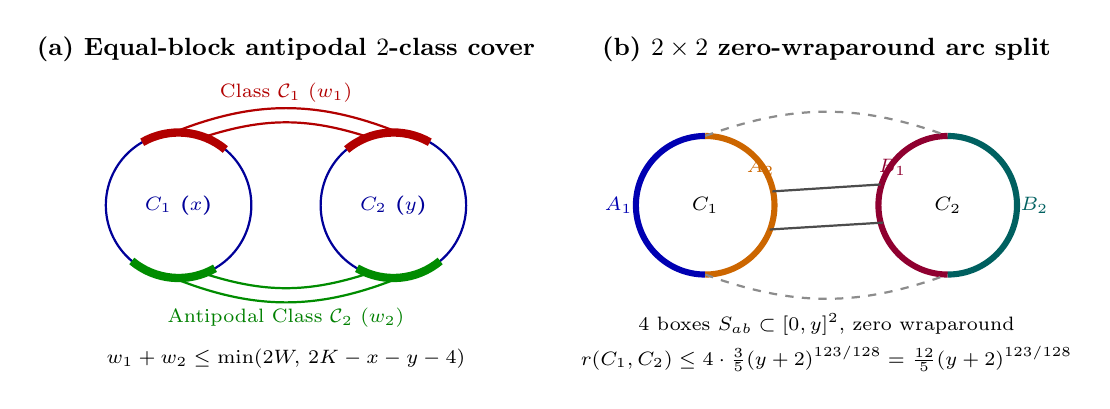
\begin{tikzpicture}[scale=0.88]
  % Left: Equal-block antipodal 2-class cover on C1, C2
  \begin{scope}[xshift=-4.4cm]
    \node[font=\small\bfseries] at (0,2.25) {(a) Equal-block antipodal $2$-class cover};
    % Cycle C1 (left circle) and C2 (right circle)
    \draw[thick,blue!60!black] (-1.55,0) circle (1.05);
    \draw[thick,blue!60!black] (1.55,0) circle (1.05);
    \node[font=\scriptsize\bfseries,blue!60!black] at (-1.55,0) {$C_1$ ($x$)};
    \node[font=\scriptsize\bfseries,blue!60!black] at (1.55,0) {$C_2$ ($y$)};
    % Class 1 (top arcs)
    \draw[line width=3pt,red!70!black] (-1.55,0) ++(50:1.05) arc (50:120:1.05);
    \draw[line width=3pt,red!70!black] (1.55,0) ++(60:1.05) arc (60:130:1.05);
    \draw[red!70!black,thick] (-1.2,0.98) to[bend left=18] (1.2,0.98);
    \draw[red!70!black,thick] (-1.65,1.04) to[bend left=22] (1.65,1.04);
    \node[font=\scriptsize,red!70!black] at (0,1.62) {Class $\mathcal{C}_1$ ($w_{1}$)};
    % Class 2 (bottom antipodal arcs)
    \draw[line width=3pt,green!55!black] (-1.55,0) ++(-130:1.05) arc (-130:-60:1.05);
    \draw[line width=3pt,green!55!black] (1.55,0) ++(-120:1.05) arc (-120:-50:1.05);
    \draw[green!55!black,thick] (-1.2,-0.98) to[bend right=18] (1.2,-0.98);
    \draw[green!55!black,thick] (-1.65,-1.04) to[bend right=22] (1.65,-1.04);
    \node[font=\scriptsize,green!50!black] at (0,-1.62) {Antipodal Class $\mathcal{C}_2$ ($w_2$)};
    \node[font=\scriptsize,align=center] at (0,-2.22) {$w_1 + w_2 \le \min(2W,\,2K-x-y-4)$};
  \end{scope}

  % Right: 2x2 arc-decomposition for Poly-k & Sublinear Circumference
  \begin{scope}[xshift=3.4cm]
    \node[font=\small\bfseries] at (0,2.25) {(b) $2 \times 2$ zero-wraparound arc split};
    % C1 split into A1, A2
    \draw[line width=2.2pt,blue!70!black] (-1.75,0) ++(90:1.0) arc (90:270:1.0);
    \draw[line width=2.2pt,orange!80!black] (-1.75,0) ++(-90:1.0) arc (-90:90:1.0);
    \node[font=\scriptsize\bfseries,blue!70!black] at (-3.0,0) {$A_1$};
    \node[font=\scriptsize\bfseries,orange!80!black] at (-0.95,0.55) {$A_2$};
    \node[font=\scriptsize] at (-1.75,0) {$C_1$};
    % C2 split into B1, B2
    \draw[line width=2.2pt,purple!75!black] (1.75,0) ++(90:1.0) arc (90:270:1.0);
    \draw[line width=2.2pt,teal!75!black] (1.75,0) ++(-90:1.0) arc (-90:90:1.0);
    \node[font=\scriptsize\bfseries,purple!75!black] at (0.95,0.55) {$B_1$};
    \node[font=\scriptsize\bfseries,teal!75!black] at (3.0,0) {$B_2$};
    \node[font=\scriptsize] at (1.75,0) {$C_2$};
    % Bridges between A2 and B1, A1 and B1, etc.
    \draw[thick,black!70] (-0.78,0.2) -- (0.78,0.3);
    \draw[thick,black!70] (-0.82,-0.35) -- (0.82,-0.25);
    \draw[thick,black!45,dashed] (-1.75,1.0) to[bend left=20] (1.75,1.0);
    \draw[thick,black!45,dashed] (-1.75,-1.0) to[bend right=20] (1.75,-1.0);
    \node[font=\scriptsize,align=center] at (0,-1.72) {$4$ boxes $S_{ab} \subset [0, y]^2$, zero wraparound};
    \node[font=\scriptsize,align=center] at (0,-2.22) {$r(C_1, C_2) \le 4 \cdot \frac{3}{5}(y+2)^{123/128} = \frac{12}{5}(y+2)^{123/128}$};
  \end{scope}
\end{tikzpicture}
\caption{(a)~Equal-block two-cycle antipodal cluster decomposition (Lemma~\ref{lem:equal-geom}), forcing $w_1 + w_2 \le \min(2W, 2K - x - y - 4)$ with zero wraparound. (b)~$2 \times 2$ arc decomposition (Section~\ref{sec:polyk}) eliminating wraparound for arbitrary disjoint cycles $C_1, C_2$.}\label{fig:twocycle}
\end{figure}

\begin{proof}[Proof of Theorem~\ref{thm:main2}]
Unequal blocks $M_2 > M_1$ are closed in Section~\ref{subsec:unequal}. For equal blocks $M_2 = M_1 = M = 2^m \ge 4$, we compare the lower bound $r \ge \mathrm{att}(M, y)$ (adjusted upward by $+1$ if $\mathrm{att}(M, y) \not\equiv x \pmod{2}$ via~\eqref{eq:bridge-parity}) against both the $1$-class upper bound $\frac{3}{5} P^{123/256}$ from~\eqref{eq:one-class} (or $F_{19}$ when widths $\le 19$) and the $2$-class upper bound~\eqref{eq:two-class} (whenever $2R \ge 0$):
\begin{enumerate}[label=(\arabic*),leftmargin=2em]
  \item \textbf{Small Blocks ($M \in \{4, 8, 16, 32, 64, 128\}$, ALL $625$ same-parity pairs):} Lean~4 kernel-verifies all $625$ pairs via the semantic reflection theorem \texttt{equal\_block\_small\_625\_sound} (\texttt{SmallEqualPairClosed}, using the conservative lower bound \texttt{exactAttachLower} and $F_{19}$ base-table fallback); \texttt{verify\_clawfree\_eg.py} independently checks all $625$ pairs using \texttt{exact\_attachment\_lower(y)} (the conservative R5 Sturmian lower bound with empty short/long band checks, distinct from the exact R11 enumerator \texttt{exact\_attachment\_r11}).
  \item \textbf{Medium Blocks ($M \in \{256, 512, 1024\}$, ALL $76{,}501$ triangular pairs):} The full triangular domains $M < x \le y \le K$ contain $3{,}655 + 14{,}535 + 58{,}311 = 76{,}501$ integer pairs, of which $9$ ($3$ per block, namely $(K-1, K-1), (K-1, K), (K, K)$) satisfy $e = K - x - 2 < 0$ and are excluded immediately by Lemma~\ref{lem:equal-geom}(ii) and $r \ge 2$. Lean~4 kernel-certifies every pair via $61$ \texttt{IBoxTree} leaves ($22 + 23 + 16$, \texttt{equal\_block\_med\_256\_512\_1024}); \texttt{verify\_clawfree\_eg.py} skips those $9$ negative-$e$ pairs and independently checks the remaining $76{,}492$ arithmetic comparisons.
  \item \textbf{Infinite Tail (ALL $M = 2^m \ge 2048$):} Normalizing $\tilde{x} = (x - M)/M$ and $\tilde{y} = (y - M)/M$ on $0 \le \tilde{x} \le \tilde{y} \le 1/3$ with $\varepsilon = 1/2048$, the four Sturmian regimes are covered by $16$ exact rational boxes (\texttt{equalTailBoxes16\_domain\_coverage}). On each box, lower-bounding the normalized attachment ratio $\rho = (1 - \alpha_R/k_R)(1 + \tilde{y}_{\mathrm{hi}}) - \frac{9}{4}\tilde{y}_{\mathrm{hi}}$ and upper-bounding the $1$-class and $2$-class factors leaves a factor $M^{10} \ge 2048^{10}$ on the lower-bound side after raising to the $256$-th power, certifying strict contradiction for ALL $M \ge 2048$ simultaneously (\texttt{equal\_block\_tail\_closure\_all\_M\_ge\_2048}, \texttt{equal\_block\_closure\_all\_pow2\_ge\_256}). \qedhere
\end{enumerate}
\end{proof}

%% =============================================================================
\section{Proof of Main Theorem 3: Poly-\texorpdfstring{$k$}{k}-Cycle 2-Factors and Sublinear Circumference}\label{sec:polyk}
%% =============================================================================

Parts~(c) and~(d) of Theorem~\ref{thm:main3} were proved in Section~\ref{subsec:r5}. We now prove parts~(a) and~(b).

\begin{lemma}[$2 \times 2$ Cycle and $1 \times 2$ Path Sublinear Bridge Bounds]\label{lem:arc-decomp}
Let $H$ be a simple cubic graph whose triangle replacement $G = T(H)$ avoids all dyadic cycles.
\begin{enumerate}[label=(\roman*),leftmargin=2.2em]
  \item For any two vertex-disjoint cycles $C_1, C_2 \subset H$ of lengths $x \le y$,
  \[
    r(C_1, C_2) \;\le\; \frac{12}{5}(y + 2)^{123/128}.
  \]
  \item For any cycle $C \subset H$ of length $y \ge 3$ and any vertex-disjoint path $Q \subset H - V(C)$ of edge-length $x \le \lfloor y/2 \rfloor$ such that every vertex of $Q$ sends at most one edge to $C$,
  \[
    r(Q, C) \;\le\; \frac{6}{5}(y + 2)^{123/128}.
  \]
\end{enumerate}
\end{lemma}

\begin{proof}
(i) Partition $V(C_1)$ into contiguous arcs $A_1 = \{0, \dots, \lfloor x/2 \rfloor - 1\}$ and $A_2 = \{\lfloor x/2 \rfloor, \dots, x - 1\}$, each of edge-length at most $\lfloor x/2 \rfloor$, and similarly split $V(C_2)$ into $B_1, B_2$ of edge-length at most $\lfloor y/2 \rfloor$ (Figure~\ref{fig:twocycle}(b)). By \texttt{two\_arc\_partition\_zero\_wraparound}, for any two vertices in the same arc $A_a$ (or $B_b$), their linear index difference equals their exact short circular distance on $C_1$ (or $C_2$). Because $H$ is cubic, bridges between $C_1$ and $C_2$ are pairwise vertex-disjoint. Hence for each of the four pairs $(a, b) \in \{1, 2\}^2$, Lemma~\ref{lem:bridge-encoding} maps the bridge set $E(A_a, B_b)$ to a valid packing $S_{ab}$ inside a square of side $W_1, W_2 \le \lfloor x/2 \rfloor + \lfloor y/2 \rfloor \le y$. Applying Theorem~\ref{thm:main1} to each $S_{ab}$ and summing over all four pairs gives
\[
  r(C_1, C_2) \;=\; \sum_{a, b \in \{1, 2\}} |S_{ab}| \;\le\; 4 \cdot \frac{3}{5}(y + 2)^{123/128} \;=\; \frac{12}{5}(y + 2)^{123/128}
\]
(\texttt{arc\_decomp\_2x2\_bridge\_bound}).

(ii) Because $Q$ is already a path of edge-length $x \le \lfloor y/2 \rfloor$ and every vertex of $Q$ has at most one bridge to $C$ (and every vertex of $C$ has degree $3$, hence at most one bridge to $Q$), the bridges between $Q$ and $C$ are pairwise vertex-disjoint. Cutting only $C$ into two arcs $B_1, B_2$ of edge-length at most $\lfloor y/2 \rfloor$ produces two valid packing instances in $[0, x + \lfloor y/2 \rfloor]^2 \subseteq [0, y]^2$, yielding $r(Q, C) \le 2 \cdot \frac{3}{5}(y + 2)^{123/128} = \frac{6}{5}(y + 2)^{123/128}$ (\texttt{arc\_decomp\_1x2\_bridge\_bound}).
\end{proof}

\begin{proof}[Proof of Theorem~\ref{thm:main3}(a)--(b)]
Assume for contradiction that $G = T(H)$ avoids all dyadic cycles.

\medskip
\noindent\textbf{(a) Universal Polynomial-$k$-Cycle 2-Factors and Equal-Block Sharpening.}
Let $C_1 \cup \dots \cup C_k$ be a spanning $2$-factor of $H$ ($k \ge 2$) with longest cycle $C_{\max}$ of length $y \ge n/k$. By Lemma~\ref{lem:r5}, $|\Vatt(C_{\max})| > \frac{3}{17} y$. On the other hand, every attachment of $C_{\max}$ is a bridge to one of the other $k - 1$ cycles, so Lemma~\ref{lem:arc-decomp}(i) gives
\[
  \frac{3}{17} y \;<\; |\Vatt(C_{\max})| \;=\; \sum_{i \neq \max} r(C_i, C_{\max}) \;\le\; (k - 1) \cdot \frac{12}{5}(y + 2)^{123/128}.
\]
Raising to the $128$-th power gives $(5 y)^{128} < (68(k - 1))^{128} (y + 2)^{123}$, which contradicts $y \ge 2^{97}(k - 1)^{128/5}$ (exact integer check at $y_0 = 2^{97}$, sharp at $2^{96}$: \texttt{universal\_y0\_97\_sharp}; fixed-$k$ exponents $k = 2, 3, 4, 5, 10 \mapsto 97, 122, 137, 148, 178$: \texttt{fixed\_k\_thresholds\_sharp}). Since $y \ge n/k$, the hypothesis $k \le (n / 2^{97})^{5/133}$ (exact form $(2^{97})^5 k^{133} \le n^5$) implies $y \ge 2^{97} k^{128/5} > 2^{97}(k - 1)^{128/5}$ and yields a contradiction (\texttt{universal\_poly\_k\_cycle\_closure}).

When all $k \in \{3, 4, 5\}$ cycles lie in the same dyadic block $(M, \lfloor 4M/3 \rfloor]$, we instead bound each of the $k - 1$ pairwise bridge counts $r(C_i, C_{\max})$ by the tighter equal-block $1$-class and $2$-class bounds~\eqref{eq:one-class}--\eqref{eq:two-class} of Lemma~\ref{lem:equal-geom}, multiplying the upper bound by $k - 1$. Repeating the normalized rational box subdivision of Section~\ref{subsec:equal} closes all $M \ge 2^{36}$ ($k = 3$, $17$ boxes), $M \ge 2^{51}$ ($k = 4$, $17$ boxes), and $M \ge 2^{62}$ ($k = 5$, $16$ boxes) (\texttt{equal\_k3\_closure\_all\_M\_ge\_2pow36}, \texttt{equal\_k4\_closure\_all\_M\_ge\_2pow51}, \texttt{equal\_k5\_closure\_all\_M\_ge\_2pow62}).

\medskip
\noindent\textbf{(b) Sublinear Circumference via R19 $+2m$ Original-Path Endpoint Pruning.}
Let $C \subset H$ be a cycle of length $y$ such that $H - V(C)$ is covered by $m \ge 1$ vertex-disjoint paths $P_1, \dots, P_m$ (so $\sum_{j=1}^m |V(P_j)| = n - y$), and suppose $y \ge \max(2^{97} m^{128/5},\, 25 n^{128/133})$.

\emph{Endpoint pruning on the original paths:} Consider any original path $P_j$ ($1 \le j \le m$). Because $H$ is cubic:
\begin{itemize}[leftmargin=1.6em]
  \item Every \emph{internal} vertex $v$ of $P_j$ already has degree $2$ inside $P_j$, so $v$ is incident to \emph{at most one} edge entering $C$.
  \item If $|V(P_j)| \ge 2$, each of the two endpoints of $P_j$ has degree $1$ inside $P_j$ and therefore sends at most $2$ edges to $C$; discarding at most $1$ excess bridge at each endpoint (at most $2$ bridges in total from $P_j$) leaves every vertex of $P_j$ incident to at most $1$ remaining bridge to $C$.
  \item If $|V(P_j)| = 1$ (a singleton $K_1$), its unique vertex sends at most $3$ edges to $C$; discarding at most $2$ excess bridges again leaves at most $1$ remaining bridge to $C$.
\end{itemize}
Across all $m$ original paths, we discard at most $2m$ bridges in total! Now partition each original path $P_j$ into consecutive vertex-disjoint subpaths $Q_{j, 1}, \dots, Q_{j, t_j}$ each containing at most $\lfloor y/2 \rfloor + 1$ vertices (hence edge-length at most $\lfloor y/2 \rfloor$). Crucially, every internal splitting vertex of $P_j$ was an \emph{internal} vertex of the original path $P_j$ and therefore ALREADY has at most $1$ surviving bridge to $C$; thus NO additional bridges are lost during splitting, and the \emph{surviving matching of bridges} between each subpath $Q_{j, i}$ and $C$ is pairwise vertex-disjoint (at most $1$ surviving bridge per vertex of $Q_{j, i}$ and, by cubicity of $H$, at most $1$ bridge per vertex of $C$), so the proof of Lemma~\ref{lem:arc-decomp}(ii) applies directly to bound the surviving bridges from $Q_{j, i}$ to $C$ by $\frac{6}{5}(y + 2)^{123/128}$!

The number of subpaths produced from $P_j$ is $t_j = \lceil |V(P_j)| / (\lfloor y/2 \rfloor + 1) \rceil \le 1 + |V(P_j)| / (\lfloor y/2 \rfloor + 1)$ (\texttt{path\_split\_subpath\_count}). Since $\lfloor y/2 \rfloor + 1 > y/2$, summing over $j = 1, \dots, m$ yields total subpath count
\[
  t \;:=\; \sum_{j=1}^m t_j \;\le\; m + \frac{2(n - y)}{y} \;\le\; m + \frac{2n}{y}
\]
(\texttt{path\_cover\_total\_subpaths}). Combining the at most $2m$ discarded endpoint bridges with the surviving-matching bound $\frac{6}{5}(y + 2)^{123/128}$ on each of the $t$ subpaths yields
\[
  \frac{3}{17} y \;<\; |\Vatt(C)| \;\le\; 2m + t \cdot \frac{6}{5}(y + 2)^{123/128}
  \;\le\; m\!\left(2 + \frac{6}{5}(y + 2)^{123/128}\right) + \frac{2n}{y}\cdot \frac{6}{5}(y + 2)^{123/128}.
\]
Split the left-hand side into $\frac{3}{17} y = \frac{3}{34} y + \frac{3}{34} y$:
\begin{itemize}[leftmargin=1.6em]
  \item For the first term: write $A := (y + 2)^{123/128}$. Since $y \ge 2^{97} m^{128/5} \ge 2^{97}$, taking $128$-th roots of the integer check $5000^{128} < 3^{128}(2^{97} + 2)^{123}$ yields $5000 < 3A$, hence $2 < \frac{6}{5000} A = \frac{1}{1000}\cdot \frac{6}{5} A$ and therefore $2 + \frac{6}{5} A < \frac{1001}{1000}\cdot \frac{6}{5} A$; combined with $(5000 \cdot 2^{97})^{128} > (68 \cdot 1001)^{128} (2^{97}+2)^{123}$, this gives $m(2 + \frac{6}{5}(y+2)^{123/128}) < \frac{3}{34} y$ (\texttt{pruning\_2m\_constants}, \texttt{PolyKAndSublinear.lean:484}).
  \item For the second term: since $y \ge 25 n^{128/133}$ and $(1 + 2/2^{97})^{123} < 2$ and $5^{128} \cdot 25^{133} \ge 2 \cdot 136^{128}$, we have $\frac{2n}{y} \cdot \frac{6}{5}(y + 2)^{123/128} \le \frac{3}{34} y$.
\end{itemize}
Adding the two inequalities contradicts $|\Vatt(C)| > \frac{3}{17} y$ (\texttt{sublinear\_circumference\_m\_path\_closure}). For any fixed $m \ge 1$ (or any $m = o(n^{5/128})$), $\max(2^{97} m^{128/5}, 25 n^{128/133}) = o(n)$; hence whenever a longest cycle $C$ of $H$ has complement covered by $m$ vertex-disjoint paths, dyadic-cycle avoidance forces $c(H) = |V(C)| < \max(2^{97} m^{128/5}, 25 n^{128/133}) = o(n)$, and by Lemma~\ref{lem:lift}(ii) ($c(G) = 3 c(H)$ and $|V(G)| = 3n$) this transfers directly to $c(G) = o(|V(G)|)$.
\end{proof}

%% =============================================================================
\section{Proof of Main Theorem 4: General \texorpdfstring{$\Delta \le 4, \delta \ge 3$}{Delta <= 4, delta >= 3} Bowtie Claw-Free Graphs}\label{sec:bowties}
%% =============================================================================

\subsection{Bowtie Forest, Simple Quotient \texorpdfstring{$F = H/H_B$}{F = H/HB}, \texorpdfstring{$\bar{d}(G) \ge 7/2$}{d-avg >= 7/2}, and Universal Transfer}\label{subsec:bowtie-forest}

\begin{proof}[Proof of Theorem~\ref{thm:main4}(a)]
Suppose $G$ is a finite simple claw-free graph with $\delta(G) \ge 3$, $\Delta(G) \le 4$, and no dyadic cycle. By Lemma~\ref{lem:repr}, $G \cong T(H)/B$ for a simple cubic graph $H$ on $N := |V(H)| \ge 4$ vertices and $b := |B|$ bowtie edges, with $|V(G)| = 3N - b$ and $2|E(G)| = 9N - 2b$. Let $H_B := (V(H), B)$ be the spanning subgraph of $H$ formed by the bowtie edges.

Observe first that for every integer $L \ge 3$ and $r \in \{0, 1, 2\}$, the interval $[L + r, 2L + r]$ contains a power of two $2^a$ ($a \ge 2$) (\texttt{bowtie\_forest\_exclusion}: let $2^a$ be the smallest power of two $\ge L + r$; since $L + r \ge 3$, $a \ge 2$ and $2^{a-1} < L + r$, so $2^a \le 2(L + r - 1) \le 2L + r$ whenever $r \le 2$). We apply this with Lemma~\ref{lem:lift}(i) three times:
\begin{enumerate}[label=(\arabic*),leftmargin=2em]
  \item \textbf{$H_B$ is a forest:} If $H_B$ contained a cycle, take a \emph{shortest} cycle $C$ in $H_B$ (length $L \ge 3$). Every edge of $C$ lies in $B$ ($k = L$), and minimality of $C$ guarantees $C$ has zero internal chords in $B$ ($m = 0$). By Lemma~\ref{lem:lift}(i), $C$ lifts to $[2L - L, 3L - L - 0] = [L, 2L]$ ($r = 0$), which hits a power of two, contradiction.
  \item \textbf{Every tree component of $H_B$ is an induced subgraph of $H$ (no edges of $E(H) \setminus B$ inside a tree of $H_B$):} If an edge $e = uv \in E(H) \setminus B$ joined two vertices in the same tree component $T$ of $H_B$, then $e$ together with the unique $u$--$v$ path in $T$ forms a simple cycle $C$ of length $L \ge 3$ with $k = L - 1$ ($r = L - k = 1$) and $m = 0$ (as $T$ is a tree, there are no chords in $B$ on $C$). Its lift window $[L + 1, 2L + 1]$ hits a power of two, contradiction.
  \item \textbf{The contracted quotient $F := H/H_B$ is simple (at most one edge of $E(H) \setminus B$ between distinct components of $H_B$):} Since every tree component of $H_B$ is induced in $H$, $F$ has no loops. If two distinct edges $e_1 = u_1 v_1, e_2 = u_2 v_2 \in E(H) \setminus B$ connected the same two distinct tree components $T_1, T_2$ of $H_B$, then $e_1, e_2$ together with the unique $u_1$--$u_2$ path in $T_1$ and unique $v_1$--$v_2$ path in $T_2$ form a simple cycle $C$ of length $L \ge 3$ with $k = L - 2$ ($r = 2$) and $m = 0$ (no edge of $B$ connects $T_1$ to $T_2$, and trees $T_1, T_2$ have no internal chords). Its lift window $[L + 2, 2L + 2]$ hits a power of two, contradiction.
\end{enumerate}
Because $H_B$ is a forest on $N$ vertices with $c := N - b \ge 1$ connected components, we have $b \le N - 1$. Therefore
\[
  \bar{d}(G) \;=\; \frac{2|E(G)|}{|V(G)|} \;=\; \frac{9N - 2b}{3N - b} \;=\; 3 + \frac{b}{3N - b} \;<\; 3 + \frac{N}{2N} \;=\; \frac{7}{2}
\]
(\texttt{davg\_lt\_seven\_halves\_of\_forest}, \texttt{davg\_ge\_seven\_halves\_no\_forest}). In particular, every claw-free graph with $\delta(G) \ge 3$, $\Delta(G) \le 4$, and $\bar{d}(G) \ge \frac{7}{2}$---including every $4$-regular claw-free graph ($\bar{d} = 4 \ge \frac{7}{2}$, \texttt{four\_regular\_satisfies\_davg\_ge\_seven\_halves})---contains a dyadic cycle. Furthermore, since $F$ is simple on $c = N - b$ vertices and has $|E(F)| = |E(H)| - b = \frac{3}{2}N - b$ edges, $\frac{3}{2}N - b \le \binom{c}{2}$ implies $c^2 - 3c \ge N$ (\texttt{simple\_quotient\_order\_bound}).

Finally, for the \textbf{Universal Cubic-to-General Transfer}: suppose $H$ contains a simple cycle $C$ of length $L = 2^K$ ($K \ge 2$). Consider the induced bowtie subgraph $H_B[V(C)]$. If $H_B[V(C)]$ contains a cycle, take a shortest such cycle $C'$ of length $L' \le L = 2^K$; its lift window $[L', 2L']$ contains a power of two $\le 2L' \le 2^{K+1}$. Otherwise $H_B[V(C)]$ is a forest on $L$ vertices, so its total number of edges (both on $C$ and internal chords of $C$) satisfies $k + m \le L - 1 = 2^K - 1$. Then by Lemma~\ref{lem:lift}(i), the lift window of $C$ satisfies
\[
  2L - k \;=\; 2^{K+1} - k \;\le\; 2^{K+1} \;\le\; 3 \cdot 2^K - (2^K - 1) \;=\; 2^{K+1} + 1
\]
more precisely $3L - k - m \ge 3 \cdot 2^K - (2^K - 1) = 2^{K+1} + 1 > 2^{K+1}$ (\texttt{dyadic\_cycle\_lift\_window}, \texttt{universal\_bowtie\_transfer}), so $2^{K+1} \in [2L - k, 3L - k - m]$ and $G$ contains a simple $C_{2^{K+1}}$.
\end{proof}

\subsection{Universal \texorpdfstring{$3$}{3}-Tree Lemma, Independent-Bowtie \texorpdfstring{$\tw(H/B) \le 3$}{tw(H/B) <= 3}, and Sharp Witness \texorpdfstring{$G_{39}$}{G39}}\label{subsec:tw3}

\begin{lemma}[Spanning $3$-Tree Completion and $15$-Line Universal $3$-Tree Lemma]\label{lem:3tree}
\leavevmode
\begin{enumerate}[label=(\roman*),leftmargin=2.2em]
  \item Every finite simple graph $F$ with $\tw(F) \le 3$ and $|V(F)| \ge 4$ is a spanning subgraph of a $3$-tree $T$ on $V(F)$ (built inductively from $K_4$ by repeatedly adding a vertex adjacent to an existing triangle).
  \item \textbf{Universal $3$-Tree Lemma (\texttt{universal\_3tree\_lemma}):} Let $T$ be a $3$-tree on $n \ge 4$ vertices and let $F \subseteq T$ be a spanning subgraph with $\delta(F) \ge 3$. Then $F$ contains at least one of the following three subgraphs:
  \begin{enumerate}[label=(\alph*),leftmargin=2em]
    \item a triangle $C_3$ containing a vertex $v$ with $d_F(v) = 3$ (\emph{degree-$3$ triangle});
    \item a subgraph isomorphic to $K_{2,3}$; or
    \item a subgraph isomorphic to $Q_3 - v^*$ (the $7$-vertex $3$-cube minus one vertex).
  \end{enumerate}
\end{enumerate}
\end{lemma}

\begin{proof}
(i) Let $(J, \{X_t\}_{t \in V(J)})$ be a tree decomposition of $F$ of width $\le 3$ ($|X_t| \le 4$). While some bag $X_t$ has $|X_t| < 4$, since $|V(F)| \ge 4$ there exists a bag containing a vertex outside $X_t$; choose a bag $s \in V(J)$ at \emph{minimum distance in $J$} from $t$ such that $X_s \not\subseteq X_t$, and pick $v \in X_s \setminus X_t$. By minimality of $\operatorname{dist}_J(t, s)$, every intermediate bag $r$ on the unique $t$--$s$ path in $J$ (excluding $s$) satisfies $X_r \subseteq X_t$, hence $|X_r| \le |X_t| \le 3$ and $v \notin X_r$. Adding $v$ to every bag on this path (excluding $s$) preserves running intersection (extending the connected subtree $J_v$ along a path attached at $s$), keeps every bag of size $\le 4$, and strictly decreases the total size deficit $\sum_{u \in V(J)} (4 - |X_u|)$. Repeating until every bag has size $4$ and contracting any edge $st$ with $X_s = X_t$, we next subdivide every tree edge $st$ with $|X_s \cap X_t| = k < 3$ into a chain of $4 - k$ bags by replacing one vertex of $X_s \setminus X_t$ by one vertex of $X_t \setminus X_s$ at each step; every vertex in $X_s \cap X_t$ stays throughout, every vertex of $X_s \setminus X_t$ stays on a prefix, and every vertex of $X_t \setminus X_s$ stays on a suffix, preserving running intersection and $|X_r| = 4$. Contracting duplicate bags gives a smooth width-$3$ tree decomposition with $|X_t| = 4$ and $|X_s \cap X_t| = 3$ on every edge $st$. Rooting $J$ at an arbitrary bag $X_{t_0}$ and traversing $J$ in preorder, each non-root bag $X_t$ (parent $X_s$) introduces a unique new vertex $v \in X_t \setminus X_s$ (running intersection forbids $v$ from having appeared earlier outside $X_s$), adjacent to the triangle $X_s \cap X_t$ of earlier vertices. Turning every bag into a $K_4$ therefore defines a spanning $3$-tree $T \supseteq F$.

(ii) Suppose $F$ avoids all three subgraphs. Let $S_0 := \{w \in V(T) : d_T(w) = 3\}$ be the set of simplicial degree-$3$ vertices of $T$, and let $S' := V(T) \setminus S_0$. For every $w \in S_0$, since $3 \le d_F(w) \le d_T(w) = 3$, we have $N_F(w) = N_T(w)$, which is a triangle in $T$. Because $F$ has no degree-$3$ triangle, $N_F(w)$ is an \emph{independent set} in $F$ (and hence $S_0$ is independent in $T$ if $|V(T)| \ge 5$, while $|V(T)| = 4 \implies F = T = K_4$ gives a degree-$3$ triangle immediately). Because $F$ has no $K_{2,3}$, the map $w \mapsto N_T(w)$ is \emph{injective} on $S_0$.

Peeling all vertices of $S_0$ from $T$ leaves a subgraph $T' := T[S']$ which is either a single triangle $K_3$ ($|S'| = 3$) or a smaller $3$-tree ($|S'| \ge 4$). If $|S'| = 3$, then $|S_0| = n - 3 \ge 2$ and every $w \in S_0$ has $N_T(w) = S'$, giving $K_{2,3}$, contradiction. Hence $|S'| \ge 4$ and $T'$ is a $3$-tree, so $T'$ has a simplicial vertex $u \in S'$ with $N_{T'}(u) = \{a, b, c\}$ (a triangle in $T'$). Since $u \notin S_0$, $u$ has at least one neighbor in $S_0$; every $w \in S_0 \cap N_T(u)$ has $N_T(w)$ a $3$-subset of $\{u, a, b, c\}$ containing $u$ (as $N_T(w) \subseteq S'$ is a clique in $T'$ containing $u$, hence contained in $\{u\} \cup N_{T'}(u) = \{u, a, b, c\}$). Thus $N_T(w) \in \{\{u, a, b\}, \{u, b, c\}, \{u, c, a\}\}$. By injectivity of $w \mapsto N_T(w)$ on $S_0$, let $k \in \{1, 2, 3\}$ be the number of such vertices $w \in S_0$ adjacent to $u$:
\begin{itemize}[leftmargin=1.6em]
  \item If $k = 1$ (say $N_T(w_1) = \{u, a, b\}$), then $u a, u b \notin E(F)$ (since $N_F(w_1)$ is independent in $F$), leaving $N_F(u) \subseteq \{w_1, c\}$, contradicting $d_F(u) \ge 3$.
  \item If $k = 2$ (say $w_1$ on $\{u, a, b\}$ and $w_2$ on $\{u, b, c\}$), then $u a, u b, u c \notin E(F)$, leaving $N_F(u) \subseteq \{w_1, w_2\}$, contradicting $d_F(u) \ge 3$.
  \item If $k = 3$ (distinct $w_1, w_2, w_3 \in S_0$ with neighborhoods $\{u, a, b\}, \{u, b, c\}, \{u, c, a\}$ in $F$), then the seven distinct vertices $\{u, w_1, w_2, w_3, a, b, c\}$ induce a subgraph of $F$ containing $Q_3 - v^*$ (edges $u w_1, u w_2, u w_3$, $w_1 a, w_1 b, w_2 b, w_2 c, w_3 c, w_3 a$), contradiction!
\end{itemize}
This entire $15$-line argument is formalized directly on \texttt{FinGraph} in \texttt{universal\_3tree\_lemma}.
\end{proof}

\begin{proof}[Proof of Theorem~\ref{thm:main4}(b) (Independent-Bowtie $\tw(H/B) \le 3$ and Sharp Witness $G_{39}$)]
Let $G$ be a finite simple independent-bowtie claw-free graph with $\delta(G) \ge 3$, $\Delta(G) \le 4$, and no $C_4$. By Lemma~\ref{lem:repr}, $G \cong T(H)/B$ where $H$ is simple cubic and $B$ is a matching of $H$, and let $F := H/B$ be the bowtie-contracted quotient (each vertex $v \in V(F)$ either corresponds to an unsplit vertex of $H$ with $d_F(v) = 3$, or to a contracted bowtie edge $b_v = v_1 v_2 \in B$ with $d_F(v) = 4$ if $F$ is simple).

\emph{Case 1: $F$ has a parallel edge (or $|V(F)| \le 3$).}
Note $F$ has no loops (since $H$ is simple and $B$ is a matching, no edge of $E(H) \setminus B$ has both endpoints in the same bowtie edge). If $F$ has two parallel edges between distinct vertices $u, v \in V(F)$, then in $H$ these two edges together with $0, 1,$ or $2$ bowtie edges from $\{b_u, b_v\}$ form a simple cycle $C$ of length $L = 2 + k$ ($k \in \{0, 1, 2\}$, $L \ge 3$ since $H$ is simple, so $k \in \{1, 2\}$) with $m = 0$ internal chordal bowties! For $k = 1$ ($L = 3$), the lift window is $[5, 8]$; for $k = 2$ ($L = 4$), the lift window is $[6, 10]$; both contain $8$ (\texttt{parallel\_edge\_hits\_c8}), giving a simple $C_8$ in $G$. If $F$ is simple, then $\delta(F) \ge 3$ forces $|V(F)| \ge 4$.

\emph{Case 2: $F$ is simple, $\delta(F) \ge 3$, $|V(F)| \ge 4$, and $\tw(F) \le 3$.}
By Lemma~\ref{lem:3tree}, $F$ contains a subgraph $F_0 \subseteq F$ isomorphic to a degree-$3$ triangle ($v_0$ has $d_F(v_0) = 3$), $K_{2,3}$, or $Q_3 - v^*$. To expand $F_0$ locally into $G = T(H)/B$, each vertex $u \in V(F_0)$ corresponds in $H$ either to:
\begin{itemize}[leftmargin=1.6em]
  \item an unsplit $H$-vertex (or one side $u_1$ of a bowtie $u_1 u_2 \in B$ when all $F_0$-edges incident to $u$ attach to $u_1$), modeled by the unsplit option $(\mathrm{row}_u, \mathrm{none})$ (possible only if $d_{F_0}(u) \le 3$); or
  \item a split bowtie $u_1 u_2 \in B$ partitioning the $F_0$-neighbors of $u$ into two nonempty sides $(S_1, S_2)$ with $1 \le |S_1|, |S_2| \le 2$ (up to swapping sides; unavailable at the fixed degree-$3$ vertex $v_0$ of a degree-$3$ triangle because $d_F(v_0) = 3$ forces $v_0$ to be unsplit in $H$!).
\end{itemize}
This yields $1 \cdot 2^2 = 4$ split configurations for a degree-$3$ triangle, $4^2 \cdot 2^3 = 128$ for $K_{2,3}$, and $4^4 \cdot 2^3 = 2{,}048$ for $Q_3 - v^*$, totaling $2{,}180$ well-formed configurations (\texttt{port\_configs\_wellFormed}).

\emph{Injective local port-witness embedding into $G$:} Let $H_0 \subseteq H$ be the local subgraph induced by the triangles corresponding to the split/unsplit choices of $V(F_0)$, and let $P(\mathrm{cfg})$ be the expanded port graph (\texttt{expandedPortGraph cfg}) where each vertex $x \in V(H_0)$ with fewer than $3$ internal edges has its remaining triangle ports padded with distinct sentinel labels ($\ge 1000$ in Lean, $< 0$ in Python) representing the external edges leaving $H_0$. We claim the canonical port map $\phi : V(P(\mathrm{cfg})) \to V(G)$ is \emph{injective} (so every simple cycle in $P(\mathrm{cfg})$ embeds as a simple cycle of the same length in $G$):
\begin{itemize}[leftmargin=1.6em]
  \item Distinct vertices $u \neq v \in V(F_0)$ are distinct vertices of $F = H/B$, so their preimage vertices in $V(H_0)$ are pairwise disjoint.
  \item Within a single triangle $T_x$ ($x \in V(H_0)$), the three ports are the three distinct vertices of $T_x$ in $G$.
  \item Across two distinct triangles $T_x, T_y$ ($x \neq y \in V(H_0)$), two ports can be identified in $G = T(H)/B$ if and only if $xy \in B$. Because $B$ is a \emph{matching}, every vertex $x \in V(H)$ belongs to at most one bowtie edge of $B$:
  \begin{enumerate}[label=(\alph*),leftmargin=1.8em]
    \item If $x \in \{u_1, u_2\}$ comes from a split vertex $u \in V(F_0)$, its unique bowtie edge is $u_1 u_2 \in B$, which is ALREADY contracted inside $P(\mathrm{cfg})$; hence its remaining (padded) port cannot be a bowtie vertex and is distinct from every port of every $T_y$ ($y \neq x$).
    \item If $x$ comes from an unsplit option for $u \in V(F_0)$, either $d_F(u) = 3$ (so $x$ has zero incident bowtie edges, and all three ports of $T_x$ are degree-$3$ vertices unique to $T_x$), or $d_F(u) = 4$ with all $F_0$-edges at $u$ attaching to $x = u_1$ (in which case the unique bowtie partner $u_2$ of $u_1$ does NOT lie in $V(H_0)$, so the padded port $w_{u_1 u_2}$ is shared only with $T_{u_2} \notin H_0$, never with any $T_y$ for $y \in V(H_0) \setminus \{x\}$!).
  \end{enumerate}
\end{itemize}
Hence $\phi : P(\mathrm{cfg}) \hookrightarrow G$ is an injective graph homomorphism! Lean~4 kernel-verifies that all $4$ degree-$3$-triangle configurations contain a simple $C_8$ (\texttt{port\_kill\_deg3\_tri\_all\_4}), all $128$ $K_{2,3}$ configurations contain a simple $C_8$ or $C_{16}$ (\texttt{port\_kill\_k23\_all\_128}), and all $2{,}048$ $Q_3 - v^*$ configurations contain a simple $C_8$ or $C_{16}$ (\texttt{port\_kill\_q3\_minus\_v\_all\_2048}).

\emph{Sharp non-planar $K_5$-minor witness $G_{39}$:} Let $F_{11}$ be the $11$-vertex graph on $\{0, \dots, 10\}$ with $18$ edges formed by joining two copies of $Q_3 - v$ at their three degree-$2$ vertices $\{0, 1, 2\}$ (Figure~\ref{fig:g39}):
\[
  E(F_{11}) \;=\; \{34, 35, 36, 40, 41, 51, 52, 62, 60,\; 78, 79, 7\text{-}10, 80, 81, 91, 92, 10\text{-}2, 10\text{-}0\}.
\]
Then $F_{11}$ has $8$ degree-$3$ vertices $\{3, \dots, 10\}$ and $3$ degree-$4$ vertices $\{0, 1, 2\}$, and admits the explicit $8$-bag width-$3$ tree decomposition with bags $\{0,1,2,3\}$, $\{0,1,3,4\}$, $\{1,2,3,5\}$, $\{0,2,3,6\}$, $\{0,1,2,7\}$, $\{0,1,7,8\}$, $\{1,2,7,9\}$, $\{0,2,7,10\}$ (and spanning $3$-tree $T_{11}$, \texttt{f11\_tw3\_certified}). Splitting the three degree-$4$ vertices as $0 \mapsto (\{4, 8\}, \{6, 10\})$, $1 \mapsto (\{4, 9\}, \{5, 8\})$, $2 \mapsto (\{5, 10\}, \{6, 9\})$ produces a simple cubic $14$-vertex graph $H_{14}$ with $3$-edge matching $B = \{(0, 1), (2, 3), (4, 5)\}$ whose expansion $G_{39} = T(H_{14})/B$ has $39$ vertices ($36$ of degree $3$, $3$ independent vertices $\{2, 7, 12\}$ of degree $4$). Lean~4 kernel-verifies on \texttt{FinGraph} (\texttt{g39\_sharp\_nonplanar\_witness}) that $G_{39}$ is induced claw-free, avoids $C_4$ and $C_8$, contains an explicit simple $C_{16}$, and that $H_{14}$ and $G_{39}$ each admit five nonempty connected pairwise vertex-disjoint branch sets forming a $K_5$ minor (in $H_{14}$: $\{0, 2, 7\}$, $\{3, 6, 8, 9\}$, $\{4, 5, 12\}$, $\{10, 11\}$, $\{1, 13\}$, lifting canonically to $G_{39}$).
\end{proof}

\begin{figure}[t]
\centering
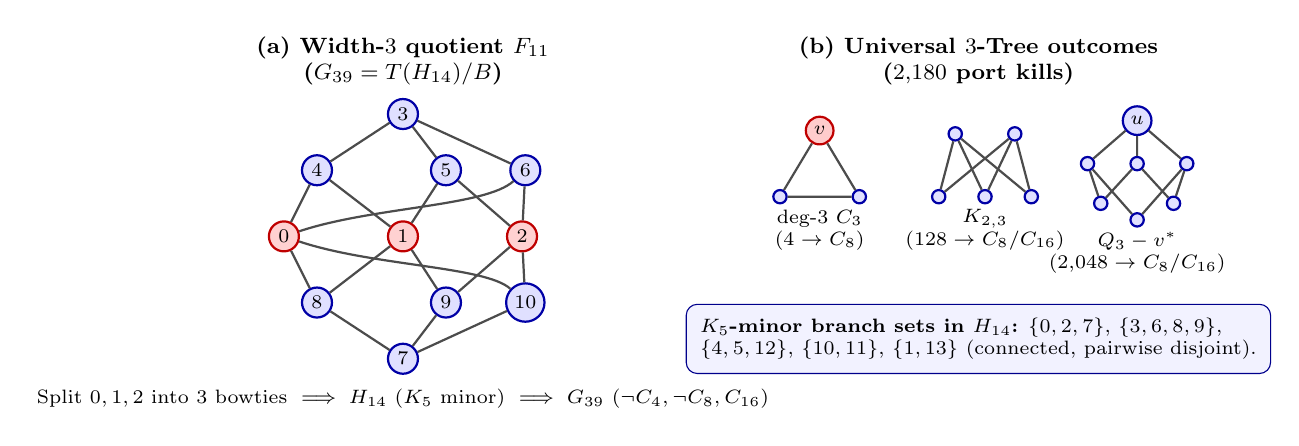
\begin{tikzpicture}[scale=0.84,
  v3/.style={circle,draw=blue!65!black,fill=blue!12,thick,inner sep=1.7pt,font=\scriptsize},
  v4/.style={circle,draw=red!75!black,fill=red!18,thick,inner sep=1.7pt,font=\scriptsize},
  ed/.style={thick,black!70}]
  % Left: Sharp witness F_11 (tw=3)
  \begin{scope}[xshift=-4.75cm]
    \node[font=\footnotesize\bfseries,align=center] at (0,2.65) {(a) Width-$3$ quotient $F_{11}$\\($G_{39} = T(H_{14})/B$)};
    \node[v4] (0) at (-1.8,0) {$0$};
    \node[v4] (1) at (0,0) {$1$};
    \node[v4] (2) at (1.8,0) {$2$};
    \node[v3] (4) at (-1.3,1.0) {$4$};
    \node[v3] (5) at (0.65,1.0) {$5$};
    \node[v3] (6) at (1.85,1.0) {$6$};
    \node[v3] (3) at (0,1.85) {$3$};
    \node[v3] (8) at (-1.3,-1.0) {$8$};
    \node[v3] (9) at (0.65,-1.0) {$9$};
    \node[v3] (10) at (1.85,-1.0) {$10$};
    \node[v3] (7) at (0,-1.85) {$7$};
    \draw[ed] (3)--(4) (3)--(5) (3)--(6) (4)--(0) (4)--(1) (5)--(1) (5)--(2) (6)--(2);
    \draw[ed] (6) .. controls (1.25,0.45) and (-0.45,0.45) .. (0);
    \draw[ed] (7)--(8) (7)--(9) (7)--(10) (8)--(0) (8)--(1) (9)--(1) (9)--(2) (10)--(2);
    \draw[ed] (10) .. controls (1.25,-0.45) and (-0.45,-0.45) .. (0);
    \node[font=\scriptsize,align=center] at (0,-2.45) {Split $0,1,2$ into $3$ bowties $\implies H_{14}$ ($K_5$ minor) $\implies G_{39}$ ($\neg C_4,\neg C_8, C_{16}$)};
  \end{scope}

  % Right: The 3 Universal 3-Tree Lemma outcomes
  \begin{scope}[xshift=3.85cm]
    \node[font=\footnotesize\bfseries,align=center] at (0.1,2.65) {(b) Universal $3$-Tree outcomes\\($2{,}180$ port kills)};
    % Outcome 1: deg-3 triangle (4 configs)
    \begin{scope}[xshift=-2.3cm,yshift=0.9cm]
      \node[v3,fill=red!20,draw=red!75!black] (a) at (0,0.7) {$v$};
      \node[v3] (b) at (-0.6,-0.3) {};
      \node[v3] (c) at (0.6,-0.3) {};
      \draw[ed] (a)--(b)--(c)--(a);
      \node[font=\scriptsize,align=center] at (0,-0.8) {deg-$3$ $C_3$\\($4 \to C_8$)};
    \end{scope}
    % Outcome 2: K_{2,3} (128 configs)
    \begin{scope}[xshift=0.2cm,yshift=0.9cm]
      \node[v3] (u1) at (-0.45,0.65) {};
      \node[v3] (u2) at (0.45,0.65) {};
      \node[v3] (w1) at (-0.7,-0.3) {};
      \node[v3] (w2) at (0,-0.3) {};
      \node[v3] (w3) at (0.7,-0.3) {};
      \foreach \u in {u1,u2} {\foreach \w in {w1,w2,w3} {\draw[ed] (\u)--(\w);}}
      \node[font=\scriptsize,align=center] at (0,-0.8) {$K_{2,3}$\\($128 \to C_8/C_{16}$)};
    \end{scope}
    % Outcome 3: Q3 - v* (2048 configs)
    \begin{scope}[xshift=2.5cm,yshift=0.9cm]
      \node[v3] (u) at (0,0.85) {$u$};
      \node[v3] (x1) at (-0.75,0.2) {};
      \node[v3] (x2) at (0,0.2) {};
      \node[v3] (x3) at (0.75,0.2) {};
      \node[v3] (y1) at (-0.55,-0.4) {};
      \node[v3] (y2) at (0.55,-0.4) {};
      \node[v3] (y3) at (0,-0.65) {};
      \draw[ed] (u)--(x1) (u)--(x2) (u)--(x3);
      \draw[ed] (x1)--(y1) (x1)--(y3) (x2)--(y1) (x2)--(y2) (x3)--(y2) (x3)--(y3);
      \node[font=\scriptsize,align=center] at (0,-1.15) {$Q_3 - v^*$\\($2{,}048 \to C_8/C_{16}$)};
    \end{scope}
    % H14 K5 minor summary box
    \node[draw=blue!55!black,fill=blue!5,rounded corners,font=\scriptsize,align=left,inner sep=5pt] at (0.1,-1.55) {%
      \textbf{$K_5$-minor branch sets in $H_{14}$:} $\{0,2,7\}$, $\{3,6,8,9\}$,\\
      $\{4,5,12\}$, $\{10,11\}$, $\{1,13\}$ (connected, pairwise disjoint).};
  \end{scope}
\end{tikzpicture}
\caption{(a)~The $11$-vertex width-$3$ quotient $F_{11}$ splitting to $H_{14}$ and $G_{39}$ (sharp non-planar $K_5$-minor witness for $C_{16}$ vs.\ $C_8$). (b)~The three mandatory subgraphs of the Universal $3$-Tree Lemma (Lemma~\ref{lem:3tree}) and their $4 + 128 + 2{,}048 = 2{,}180$ expanded-port kills.}\label{fig:g39}
\end{figure}

\subsection{Dyadic-Cycle-Free Independent-Bowtie Order Bound \texorpdfstring{$|V(G)| \ge 120$}{|V(G)| >= 120}}\label{subsec:order120}

\begin{proof}[Proof of Theorem~\ref{thm:main4}(c)]
Let $G = T(H)/B$ be a \emph{dyadic-cycle-free} independent-bowtie claw-free graph with $\delta(G) \ge 3$, $\Delta(G) \le 4$, and $4$-regular simple quotient $F = H/B$ (by Theorem~\ref{thm:main4}(a)). Setting $c := |V(F)|$, every vertex of $F$ is a contracted bowtie edge of the perfect matching $B$, so $|V(H)| = 2c$, $|B| = c$, and $|V(G)| = 3(2c) - c = 5c$ (\texttt{indep\_bowtie\_4reg\_order\_5c}). It suffices to prove $c \ge 24$.

\medskip
\noindent\textbf{Step 1: Lifted quotient-cycle switch counts and merged-cycle kills.}
Any simple $r$-cycle $C_F$ in $F$ ($r \ge 3$) lifts uniquely to a simple cycle $C_H$ in $H$ of length $L = r + s$, where $s \in [0, r]$ is the number of vertices of $C_F$ at which the two cycle edges attach to \emph{opposite} sides of the vertex's bowtie edge (\emph{switches}). Crucially, because $B$ is a matching and $C_F$ is simple, $C_F$ visits each quotient vertex at most once, so $C_H$ uses $k = s$ bowtie edges on $C_H$ and has \emph{$m = 0$ internal chordal bowties} (the partner of any unswitched vertex of $C_H$ lies strictly outside $V(C_H)$!). Thus $C_H$ lifts to $[2L - s, 3L - s] = [2r + s, 3r + 2s]$ in $G$. Checking dyadic-cycle avoidance across $r \in \{3, \dots, 8\}$ restricts the permissible switch count $s$ to the exact table (\texttt{indep\_bowtie\_120\_arithmetic\_bundle}):
\[
  s(3) \in \{3\},\quad s(4) \in \{1\},\quad s(5) \in \{0\},\quad s(6) \in \{5, 6\},\quad s(7) \in \{3, 4, 5\},\quad s(8) \in \{1, 2, 3\}.
\]
Next, suppose two simple cycles $C_a, C_b$ in $F$ ($a \in \{3, 4\}$, $b \in \{3, \dots, 8\}$) share \emph{only} a single vertex $v \in V(F)$ and BOTH switch at $v$. In $H$, their lifts $C_a', C_b'$ share the single bowtie edge $b_v = v_1 v_2 \in B$ and are otherwise vertex-disjoint; their symmetric difference $C_a' \triangle C_b'$ is a simple cycle in $H$ of length $L = (a + s_a) + (b + s_b) - 2$, using $k = s_a + s_b - 2$ bowtie edges on the cycle, and having \emph{exactly $m = 1$ internal chordal bowtie} (namely $b_v$ itself, since $B$ is a matching and no other bowtie can connect $V(C_a') \setminus \{v_1, v_2\}$ to $V(C_b') \setminus \{v_1, v_2\}$!). By \texttt{indep\_bowtie\_120\_arithmetic\_bundle}, for EVERY permissible $(a, b, s_a, s_b)$ with $s_a, s_b \ge 1$, the lift window $[2L - k, 3L - k - 1]$ hits a power of two!

\medskip
\noindent\textbf{Step 2: Local subgraph exclusions ($360{,}612$ lifted-$H$ + $166$ overlap patterns).}
From Step~1 and exhaustive split enumeration in \texttt{verify\_clawfree\_eg.py} (\texttt{verify\_theorem4c\_independent\_bowtie\_120}, $12$ subgraph families totaling $360{,}612$ configurations plus all $166 = 9 + 27 + 75 + 55$ labeled single-edge-overlap configurations with extra shared vertices for $(C_4, C_6)$, $(C_5, C_6)$, $(C_6, C_6)$, $(C_5, C_7)$):
\begin{enumerate}[label=(\roman*),leftmargin=2em]
  \item \emph{Triangles, squares, and pentagons sharing an edge:}
  \begin{itemize}[leftmargin=1.4em]
    \item Two triangles sharing an edge $xy$ form an outer $4$-cycle which switches at both off-edge vertices (since each triangle has $s(3) = 3$), giving $s(4) \ge 2$, contradicting $s(4) = 1$. Since two triangles also cannot share only one vertex (both switch there, killed by Step~1), \emph{all triangles of $F$ are pairwise vertex-disjoint}.
    \item A triangle $T = (x, y, z)$ and a $4$-cycle $Q$ sharing an edge $xy$ (with $z \notin V(Q)$; if $z \in V(Q)$ then $Q$ contains a second triangle sharing an edge with $T$) form an outer $5$-cycle that switches at $z$, contradicting $s(5) = 0$.
    \item A triangle $T = (x, y, z)$ and a $5$-cycle $P$ sharing only an edge $xy$ (with $z \notin V(P)$; if $z \in V(P)$ then $P$ contains a triangle or $4$-cycle sharing an edge with $T$) form an outer $6$-cycle whose three internal vertices of $P \setminus \{x, y\}$ do not switch ($s(5) = 0$), so the outer $6$-cycle has at most $3$ switches, contradicting $s(6) \in \{5, 6\}$.
    \item Every $5$-cycle has $s(5) = 0$: entering any vertex $w$ of a $5$-cycle along an edge on one side of the bowtie $b_w$, the $5$-cycle \emph{must} exit along the unique other edge on that same side! Consequently, \emph{any two $5$-cycles sharing an edge coincide} (following the unique same-side continuation around all $5$ vertices), and \emph{no $5$-cycle can share an edge with a $4$-cycle} (a $4$-cycle has $s(4) = 1$, so entering the $4$-cycle along any of its edges and following same-side continuations through its three non-switch vertices arrives at the unique switch vertex $w^*$ on the two opposite sides of $b_{w^*}$, contradicting the $5$-cycle's same-side continuation!).
    \item Two $4$-cycles sharing a single edge $xy$ (with disjoint remaining vertices) form an outer $6$-cycle having at most $4$ switches (each of the two remaining vertices of each $4$-cycle contributes at most $1$ switch, and in fact at most $2$ switches total outside $\{x, y\}$ plus at most $2$ at $\{x, y\}$), contradicting $s(6) \in \{5, 6\}$; two $4$-cycles sharing a $2$-path give $K_{2,3}$, which has no valid bowtie expansion (already killed by $128$ port kills in Section~\ref{subsec:tw3}, and excluded by $s(4) = 1$).
  \end{itemize}
  \item \emph{Girth-$9$ Complementary Triangle Barrier:} At any vertex $v$ of a triangle $T = (v, u_1, u_2)$ in $F$, the two complementary neighbors $u_3, u_4 \notin T$ attach to opposite sides of $b_v$ (because $T$ switches at $v$). Hence any shortest path $P$ in $F - \{v\}$ between $u_3$ and $u_4$ of length $\le 6$ either avoids $\{u_1, u_2\}$---forming a switching cycle $C_b$ ($b \le 8$) sharing only $v$ with $T$, killed by Step~1 (\texttt{C3+C3..C8 share v})---or hits $\{u_1, u_2\}$ at a first vertex at distance $\le 3$ from one of $u_3, u_4$, forming a simple cycle of length $\le 5$ sharing an edge with $T$, ruled out by~(i)! Thus $\operatorname{dist}_{F - \{v\}}(u_3, u_4) \ge 7$.
  \item \emph{Single-edge overlaps and two-square bridges:} No pair $(C_4, C_6)$, $(C_5, C_6)$, $(C_6, C_6)$, or $(C_5, C_7)$ can share a single edge (neither with disjoint remaining vertices---killed in the $360{,}612$ sweep---nor with additional shared vertices---killed across all $166$ labeled overlap graphs!). Nor can two $4$-cycles meeting at $v$ be joined by an edge (\texttt{2xC4 + edge}) or a $2$-path (\texttt{2xC4 + 2-path}) between their opposite corners.
\end{enumerate}

\medskip
\noindent\textbf{Step 3: Distance-$3$ neighborhood count ($c \ge 24$).}
Fix a root vertex $v \in V(F)$ with $N_1(v) = \{u_1, u_2, u_3, u_4\}$, and let $N_2(v)$ and $N_3(v)$ be the sets of vertices at distance $2$ and $3$ from $v$ in $F$.
\begin{itemize}[leftmargin=1.6em]
  \item \textbf{Case 1 ($F$ contains a triangle $T = (v, u_1, u_2)$):} By~(i)--(ii), no other triangle touches $v$, no $4$-cycle uses $\{u_3, u_4\}$ (else $\operatorname{dist}_{F-v}(u_3, u_4) \le 2 < 7$), and no $4$-cycle uses $u_1$ or $u_2$ with another neighbor of $v$ (else a $4$-cycle sharing an edge with $T$, or if through $u_1, u_3$ giving a $4$-cycle sharing $v u_1$ with $T$). Thus $|N_2(v)| = 2 + 2 + 3 + 3 = 10$, partitioned into pairwise disjoint sets $A = N(u_1) \setminus \{v, u_2\}$, $B = N(u_2) \setminus \{v, u_1\}$, $C = N(u_3) \setminus \{v\}$, $D = N(u_4) \setminus \{v\}$ ($|C| = |D| = 3$). Any edge from $C \cup D$ to $A \cup B$ closes a $5$-cycle sharing an edge ($v u_1$ or $v u_2$) with $T$, impossible by~(i); any edge between $C$ and $D$, or any common neighbor of $C$ and $D$ in $N_3(v)$, gives a $u_3$--$u_4$ path of length $\le 4$ in $F - \{v\}$, impossible by~(ii). Thus $N_3(C)$ and $N_3(D)$ are disjoint subsets of $N_3(v)$, and all $9$ outgoing stubs from $C$ go to $C \cup N_3(C)$ (and symmetrically for $D$). If $C$ has an internal edge $xy$, then $(u_3, x, y)$ is a triangle, using $2$ stubs of $C$ and leaving $7$ stubs to $N_3(C)$; all $7$ endpoints in $N_3(C)$ are distinct (any collision between two vertices of $C$ forms a $4$-cycle sharing an edge with $(u_3, x, y)$, ruled out by~(i)). If $C$ is independent, all $9$ stubs go to $N_3(C)$, and at most one pair of stubs can collide at a vertex of $N_3(C)$ (two collisions at the same vertex give $K_{2,3}$, and two collisions at distinct vertices give two $4$-cycles sharing an edge at $u_3$, both ruled out by~(i)), leaving $|N_3(C)| \ge 7$ (and symmetrically $|N_3(D)| \ge 7$). Hence $c \ge 1 + 4 + 10 + 7 + 7 = 29$.
  \item \textbf{Case 2 ($F$ is triangle-free):} Every $4$-cycle through $v$ uses two edges incident to $v$. By~(i), no two $4$-cycles share an edge at $v$, so $v$ lies on $0, 1,$ or $2$ edge-disjoint $4$-cycles. Moreover, every edge inside $N_2(v)$ closes a $5$-cycle through $v$ (its endpoints cannot share a common parent in $N_1(v)$ since $F$ is triangle-free), using two edges incident to $v$; by~(i), distinct $5$-cycles cannot share an edge and no $5$-cycle can share an edge with a $4$-cycle!
  \begin{itemize}[leftmargin=1.4em]
    \item \emph{$0$ $4$-cycles at $v$:} $|N_2(v)| = 12$ ($36$ outgoing stubs from $N_2(v)$). Because the $4$ edges incident to $v$ can support at most $2$ edge-disjoint $5$-cycles through $v$, at most $2$ edges lie inside $N_2(v)$ ($4$ stub endpoints), leaving $\ge 36 - 4 = 32$ stubs into $N_3(v)$. Since $F$ is $4$-regular, $|N_3(v)| \ge \lceil 32 / 4 \rceil = 8$, giving $c \ge 1 + 4 + 12 + 8 = 25$.
    \item \emph{$1$ $4$-cycle at $v$:} $|N_2(v)| = 11$ ($32$ outgoing stubs: $2$ from the $4$-cycle corner and $3$ from each of the other $10$ vertices). Because the $4$-cycle uses $2$ edges incident to $v$ and no $5$-cycle can share an edge with it, only the $2$ remaining edges at $v$ can support a $5$-cycle through $v$; hence at most $1$ edge lies inside $N_2(v)$ ($2$ stub endpoints), leaving $\ge 32 - 2 = 30$ stubs into $N_3(v)$, so $|N_3(v)| \ge \lceil 30 / 4 \rceil = 8$, giving $c \ge 1 + 4 + 11 + 8 = 24$.
    \item \emph{$2$ edge-disjoint $4$-cycles at $v$:} Say $Q_1 = (v, u_1, w_{12}, u_2)$ and $Q_2 = (v, u_3, w_{34}, u_4)$, with $|N_2(v)| = 10$ consisting of $w_{12}, w_{34}$ and four $2$-sets $A, B, C, D$ of free children under $u_1, u_2, u_3, u_4$. Because all $4$ edges incident to $v$ belong to $Q_1 \cup Q_2$ and no $5$-cycle can share an edge with a $4$-cycle, \emph{zero} edges lie inside $N_2(v)$! Thus all outgoing stubs from $w_{12}$ ($2$), $A \cup B$ ($12$), $w_{34}$ ($2$), and $C \cup D$ ($12$) go to $N_3(v)$, and $4$-regularity gives $|N_3(w_{12})| = 2$, $|N_3(A \cup B)| \ge \lceil 12/4 \rceil = 3$, $|N_3(w_{34})| = 2$, and $|N_3(C \cup D)| \ge 3$. We verify that all four third-layer sets are pairwise disjoint:
    \begin{enumerate}[label=(\alph*),leftmargin=1.6em]
      \item \emph{$w_{12}$ vs.\ $A \cup B$ (same half):} A common neighbor $z$ of $w_{12}$ and $a \in A$ forms the $4$-cycle $(u_1, w_{12}, z, a)$ sharing edge $u_1 w_{12}$ with $Q_1$, ruled out by~(i) (symmetrically $w_{34}$ vs.\ $C \cup D$).
      \item \emph{$w_{12}$ vs.\ $w_{34}$ (opposite corners):} A common neighbor $z$ forms a $2$-path between the opposite corners of $Q_1$ and $Q_2$, killed by \texttt{2xC4 + 2-path} in~(iii).
      \item \emph{$A \cup B$ vs.\ $C \cup D$ (free children across halves):} A common neighbor $z$ of $a \in A$ and $c \in C$ forms the $6$-cycle $(v, u_1, a, z, c, u_3)$ sharing the single edge $v u_1$ with $Q_1$, killed by \texttt{C4+C6 share 1e} (including all extra-vertex overlaps) in~(iii).
      \item \emph{$w_{12}$ vs.\ $C \cup D$ (corner vs.\ opposite free child):} A common neighbor $z$ of $w_{12}$ and $c \in C$ yields the $6$-cycle $(v, u_1, w_{12}, z, c, u_3)$ sharing the single edge $v u_3$ with $Q_2$, again killed by \texttt{C4+C6 share 1e} in~(iii) (symmetrically $w_{34}$ vs.\ $A \cup B$).
    \end{enumerate}
    Hence $c \ge 1 + 4 + 10 + (2 + 3 + 2 + 3) = 25$.
  \end{itemize}
\end{itemize}
Taking the minimum across all four cases gives $c \ge \min(29, 25, 24, 25) = 24$ and $|V(G)| = 5c \ge 120$ (\texttt{indep\_bowtie\_120\_arithmetic\_bundle}).
\end{proof}

\subsection{Tier-1 Hamiltonian All-Chord-\texorpdfstring{$B$}{B} Theorems}\label{subsec:ham}

\begin{proof}[Proof of Theorem~\ref{thm:main4}(d)]
Let $H = C_N \cup M$ ($N \ge 4$ even, $V(C_N) = \mathbb{Z}_N$) with perfect matching $M$ of chords of $C_N$, and set $G = T(H)/M$. Every simple cycle $C$ of length $L$ in $H$ using $k$ matching chords and enclosing $m$ additional internal matching chords has lift window $[2L - k, 3L - k - m]$ (Lemma~\ref{lem:lift}(i)). Because the $k$ chords occupy $2k$ vertices of $C$, the remaining $L - 2k$ vertices pair into at most $\lfloor (L - 2k)/2 \rfloor$ internal chords, giving the universal conservative upper endpoint $3L - k - \lfloor (L - 2k)/2 \rfloor = \lceil 5L/2 \rceil$ (for $k = 0$, $[2N, 5N/2]$; for $k = 1$, $[2L - 1, \lceil 5L/2 \rceil]$; for $k = 2$, $[2L - 2, \lceil 5L/2 \rceil]$). Assume $G$ avoids all dyadic cycles.

\medskip
\noindent\textbf{1. Two-chord girth $L_2 \ge 10$.}
For any $2$-chord cycle of length $L \in \{4, 5, 7, 8, 9\}$ and every $0 \le m \le \lfloor (L - 4)/2 \rfloor$, the lift window $[2L - 2, 3L - 2 - m]$ hits $8$ or $16$ (\texttt{ham\_all\_chord\_b\_L2\_ge\_10}). At $L = 6$, the only window avoiding powers of two is $[10, 15]$ (requiring $m = 1$ internal chord, since $m = 0$ gives $[10, 16]$ hitting $16$). However, a $2$-chord $6$-cycle consists of two disjoint rim arcs of lengths summing to $4$ (so $(1, 3)$ or $(2, 2)$) and one internal chord between their two interior vertices: if $(1, 3)$, the interior of the length-$3$ arc has two adjacent vertices, so joining them creates a rim edge rather than a chord; if $(2, 2)$, joining the two midpoints creates a $2$-chord $4$-cycle (window $[6, 10]$ hitting $8$!). Hence every $2$-chord cycle has length $L_2 \ge 10$.

\medskip
\noindent\textbf{2. Local short-chord strip exclusion ($W \le 31$, $L_{\mathrm{win}} = 17$).}
Suppose a contiguous rim window $\{0, 1, \dots, L_{\mathrm{win}} - 1\}$ has every incident chord of short span $s \in [2, W]$ (with $1$-chord window avoiding powers of two) and $N > L_{\mathrm{win}} + 2W$. Then the window plus all possible chord endpoints embeds injectively in $[-W, L_{\mathrm{win}} - 1 + W]$ with zero cyclic wraparound (at $W = 31, L_{\mathrm{win}} = 17$, the strip has $17 + 2 \cdot 24 \le 65$ active labels since the largest permissible span $\le 31$ is $24$, and even nominal offsets through $31$ use $79 < 102$ labels, embedding injectively whenever $N > 102$). Two chords in the strip whose four endpoints are not separated form a $2$-chord cycle of length $r_1 + r_2 + 2$ inside the strip, which must satisfy $L_2 \ge 10$ and avoid powers of two. Furthermore, for any chord $(a, b)$ with $0 \le a < b < L_{\mathrm{win}}$, its exact number of internal chords is at most the number of already-assigned internal chords plus $\lfloor u_{\mathrm{int}}/2 \rfloor$ where $u_{\mathrm{int}}$ is the count of still-unmatched interior vertices. Minimum-domain backtracking in \texttt{verify\_clawfree\_eg.py} (\texttt{local\_strip}) exhaustively eliminates $(W, L_{\mathrm{win}}) = (7, 4)$ ($9$ visits), $(15, 8)$ ($113$ visits), and $(31, 17)$ ($29{,}357$ visits, $0$ survivors). Thus for every $N > 102$, every one of the $N$ sliding $17$-vertex rim windows meets at least one long chord of span $\ge 32$; since each long chord has $2$ endpoints and therefore meets at most $2 \cdot 17 = 34$ sliding $17$-vertex windows, double-counting forces at least $\lceil N/34 \rceil$ long chords!

\medskip
\noindent\textbf{3. Universal $4$-Tier Dyadic-Octave Coverage and $39$ All-Order Periods.}
Suppose $M$ is invariant under rotation by $k$ ($k \mid N$; note if $M$ is invariant under rotation by $k \nmid N$, it is invariant under $\gcd(k, N) \mid N$). For any chord $e = (u, u + s)$ of span $s \le N/2$, if $1 \le j$ satisfies $j k < s$, then $e$ and its translate $e' = (u + jk, u + s + jk)$ are disjoint and form a $2$-chord cycle of length $2jk + 2$ using the two disjoint rim arcs of length $jk$ between their endpoints, whose conservative lift window contains $[4jk + 2, 5jk + 5]$!
\begin{itemize}[leftmargin=1.6em]
  \item \emph{Universal translate cutoff ($j \in \{4, 5, 6, 7\}$):} Because $4(j + 1) \le 5j$ for $j \in \{4, 5, 6\}$, the union $\bigcup_{j=4}^7 [4jk + 2, 5jk + 5]$ covers the contiguous interval $[16k + 2, 35k + 5]$ whose upper endpoint strictly exceeds twice its lower endpoint ($35k + 5 > 2(16k + 2)$), hence ALWAYS contains a power of two! Therefore, NO chord in a $k$-periodic matching can have span $s > 7k$ (the \emph{seventh-translate bound}).
  \item \emph{Odd periods $g \mid N$ ($N = m g$, $m \ge 2$ even) and $4$-Tier Dyadic-Octave:} The involution induced by $M$ on the odd number $g$ of residue classes mod~$g$ must fix at least one residue class $r_0$ (rotating to $r_0 = 0$). Since the matching step $d$ on class $0$ satisfies $d \equiv 0 \pmod{g}$, $d \not\equiv 0 \pmod{N}$, and $2d \equiv 0 \pmod{N}$, class $0$ MUST use the antipodal chord of span $N/2 = (m/2) g$! By the seventh-translate bound applied to this antipodal chord, $(m/2)g \le 7g$, i.e., $m \le 14$; moreover, at $m = 14$ ($N = 14g$, $1$-chord cycle length $L = 7g + 1$), the antipodal $1$-chord window $[2(7g + 1) - 1,\, \lceil 5(7g + 1)/2 \rceil] = [14g + 1,\, (35g + 5)/2]$ (exact for odd $g$) overlaps the $j = 4, 5, 6$ translate union $[16g + 2, 30g + 5]$ (since $16g + 2 \le (35g + 5)/2$), giving the contiguous interval $[14g + 1, 30g + 5]$ whose upper endpoint satisfies $30g + 5 \ge 2(14g + 1)$ for all $g \ge 1$, forcing a power of two at $m = 14$ as well! Thus EVERY surviving odd-period order satisfies $m \in \{2, 4, 6, 8, 10, 12\}$.
  
  Furthermore, for every power of two $P = 2^a \ge 16$ and odd period $g \mid N$ ($N = mg$ even), Lean~4 kernel-proves (\texttt{ham\_all\_chord\_b\_4tier\_octave\_universal}) the exact lift-window hits and overlap of three octave tiers:
  \begin{align*}
    A_a &= \bigl[\lfloor(4P-1)/5\rfloor,\, P-1\bigr], &
    B_a &= \bigl[\lfloor(8P+14)/15\rfloor,\, \lfloor(8P-2)/12\rfloor\bigr],\\
    C_a &= \bigl[\lfloor(16P+24)/25\rfloor,\, \lfloor(16P-2)/20\rfloor\bigr]. & &
  \end{align*}
  Specifically: for every odd $g \in A_a$, the antipodal $1$-chord window at $m = 2$ hits $2P$ ($2g + 1 \le 2P \le \lfloor(5g + 5)/2\rfloor$) and the $j = 1$ translate window at all $m \ge 4$ hits $4P$ ($4g + 2 \le 4P \le 5g + 5$), closing $100\%$ of all even multiples $m \ge 2$ across $A_a$ (which has asymptotic density $\frac{P/5}{P/2} = \frac{2}{5} = 40\%$ among odd periods in each dyadic octave $[P/2, P]$, subject to endpoint rounding such as $4/8$ at $P = 32$); for $g \in B_a$, the rim window at $m = 6$ ($[12g, 15g]$) and $j = 3$ translate window at $m \ge 8$ ($[12g + 2, 15g + 5]$) both hit $8P$, closing all $m \ge 6$; for $g \in C_a$, the rim window at $m = 10$ ($[20g, 25g]$) and $j = 5$ translate window at $m \ge 12$ ($[20g + 2, 25g + 5]$) both hit $16P$, closing all $m \ge 10$; and the overlaps $b_{\mathrm{hi}} + 1 \ge c_{\mathrm{lo}}$ and $c_{\mathrm{hi}} \ge a_{\mathrm{lo}}$ unite the full joined interval $B_a \cup C_a \cup A_a = [\lfloor(8P + 14)/15\rfloor, P - 1]$ for all even $m \ge 10$ (note that tiers $A_a, B_a, C_a$ apply for $m \ge 2, 6, 10$ respectively; e.g., at $P = 128$, $g = 93 \in C_7 \setminus (A_7 \cup B_7)$ has no rim, antipodal, or translate hit at $m = 6$).
  \item \emph{Closing all $39$ all-order periods:}
  \begin{enumerate}[label=(\alph*),leftmargin=1.8em]
    \item \emph{Six short even periods $k \in \{2, 4, 6, 10, 12, 14\}$:} Each has a small translate $j k \le 31$ whose window $[4jk + 2, 5jk + 5]$ hits a power of two (specifically $j = 3$ for $k = 2$ hits $32$; $j = 3, 2, 1$ for $k = 4, 6, 12$ hit $64$; $j = 3, 2$ for $k = 10, 14$ hit $128$), capping every chord span at $\le j k \le 31$ and contradicting the $W \le 31$ strip exclusion for $N > 102$ (while $N \le 102$ is closed unconditionally below).
    \item \emph{Even period $k = 8$:} By the seventh-translate bound, every chord span satisfies $s \le 7 \cdot 8 = 56$. Fixed residue classes mod~$8$ require antipodal chords of span $N/2 \le 56$ with $16 \mid N$ (so $N \in \{16, 32, 48, 64, 80, 96, 112\}$): at $N = 112$, the antipodal $1$-chord window $[113, 143]$ hits $128$, while all even $N \le 102$ (including $N = 96$, where the $1$-chord window $[97, 123]$ misses a power of two) are already closed unconditionally by the arbitrary-matching search below. For $N \ge 168$, the strip $[-56, 38 + 56] = [-56, 94]$ has width $151 < 168$ ($2 \cdot 56 + 7 + 31 = 150 < 168$) and embeds injectively into $C_N$; exhaustive residue-matching search (\texttt{period\_eight(None)}, $1{,}781$ nodes) eliminates all $N \ge 168$, and exact cyclic searches eliminate every multiple $N \in \{104, 112, 120, 128, 136, 144, 152, 160\}$ (with $N \le 102$ closed below).
    \item \emph{All $32$ odd periods $g \in \{1, 3, 5, \dots, 63\}$:} Filtering $m \in \{2, 4, 6, 8, 10, 12\}$ with $N = m g > 128$ against the rim window $[2N, 5N/2]$, the antipodal $1$-chord window, and the translate windows $1 \le j < m/2$ leaves exactly $23$ open $(g, m)$ pairs, all eliminated with $0$ survivors by fixed-residue-0 constraint propagation (\texttt{close\_odd\_order}, $93{,}902$ nodes).
  \end{enumerate}
  Together, $\{2, 4, 6, 8, 10, 12, 14\} \cup \{1, 3, \dots, 63\}$ give all $39$ all-order periods (\texttt{ham\_all\_chord\_b\_tier1\_periods\_39}).
\end{itemize}

\medskip
\noindent\textbf{4. Arbitrary-matching closure for ALL even $4 \le N \le 136$.}
By dihedral symmetry of $C_N$, rotate and reflect any surviving perfect matching $M$ so that a chord of \emph{minimum} span $s_{\min}$ connects $0$ to $s_{\min}$; every other chord in $M$ then has span $\ge s_{\min}$ and is compatible with $(0, s_{\min})$.
\begin{itemize}[leftmargin=1.6em]
  \item For all even $4 \le N \le 102$: minimum-domain backtracking over compatible chords reaches $641$ terminal leaves (all at $N \in \{82, 84, 86\}$), and exact internal-chord evaluation on all $1$-chord and $2$-chord cycles eliminates every leaf ($0$ survivors).
  \item For all even $104 \le N \le 128$ ($N = 2k$, $52 \le k \le 64$): the Hamiltonian rim $C_N$ itself ($k$ internal chords) has lift window $[2N, 3N - k] = [4k, 5k] \ni 256$ (\texttt{ham\_all\_chord\_b\_rim\_c256\_104\_to\_128}), closing every matching unconditionally!
  \item For $N \in \{130, 132, 134, 136\}$: exact arbitrary-matching backtracking with minimum-span anchoring and conservative $2$-chord compatibility closes every order with $0$ survivors in $\{130: 73,\; 132: 236,\; 134: 242,\; 136: 723\}$ visits (\texttt{matching\_frontier}). \qedhere
\end{itemize}
\end{proof}

%% =============================================================================
\section{Formal Verification Architecture, Traceability, and Reproducibility}\label{sec:verification}
%% =============================================================================

The complete Lean~4 library, standalone Python~3 verifiers, deterministic JSON witness bundles, and SHA-256 manifest are bundled under \texttt{paper2\_clawfree/} and archived alongside Paper~1 upon publication release at \url{https://github.com/lollipoll/erdos-gyarfas}.

\begin{itemize}[leftmargin=1.8em]
  \item \textbf{Pure Lean~4 Kernel Library (\texttt{lean/}, \texttt{v4.36.0}, ZERO Mathlib, ZERO \texttt{Std}):} $13$ modules plus root \texttt{ClawFreeEG.lean} and \texttt{AxiomCheck.lean}. A serialized cold build from empty \texttt{.lake} (\texttt{LEAN\_NUM\_THREADS=1 lake build}, $30$ jobs) completes with exit code $0$ and $0$ warnings in ${\sim}6\text{m}\,30\text{s}$ at peak RSS $1{,}393{,}452\,\mathrm{KiB}$ ($1.33\,\mathrm{GiB} < 1.50\,\mathrm{GiB}$). All $261/261$ public theorems in \texttt{AxiomCheck.lean} depend solely on $\{\texttt{propext}, \texttt{Classical.choice}, \texttt{Quot.sound}\}$, with zero \texttt{sorry}, zero \texttt{admit}, zero custom axioms, zero \texttt{native\_decide}, zero \texttt{unsafe}/\texttt{partial}, and zero \texttt{set\_option} overrides.
  \item \textbf{Standalone Zero-Float Python Verifiers (\texttt{cert/}):} Both scripts are pure Python~3 stdlib, AST-guarded against floats and true division \texttt{/}, and guarded against \texttt{python3 -O} optimization bypass:
  \begin{enumerate}[label=(\alph*),leftmargin=2em]
    \item \texttt{cert/verify\_clawfree\_eg.py} replays all six certificate suites in ${\sim}31\,\mathrm{s}$ (peak RSS ${\sim}133\,\mathrm{MiB}$), regenerating all four JSON witness bundles in \texttt{cert/witnesses/} byte-for-byte identically;
    \item \texttt{cert/verify\_clawfree\_parity.py} (invoked with \texttt{--check-axioms <sysroot>}) verifies the AST zero-float/zero-\texttt{/}/zero-\texttt{research} audit, the $15$-file Lean trust-token scan (including \texttt{AxiomCheck.lean}), live $261/261$ axiom auditing, and literal data parity across Lean, Python, and JSON ($F_{19} = 210$, Case~B $= 813$, \texttt{IBoxTree} $= 46 + 61$, tail boxes $= 16$, equal-$k$ boxes $= 50$, port witnesses $= 2{,}180$, $G_{39}/H_{14}/F_{11}$, $39$ periods, $23$ odd open cases).
  \end{enumerate}
\end{itemize}

Table~\ref{tab:traceability} records the four-layer traceability matrix of principal declarations across all four Main Theorems (the complete $261$-theorem index is audited in \texttt{lean/AxiomCheck.lean}; each Lean umbrella certifies the discrete arithmetic and finite-certificate core of its corresponding theorem rather than quantifying over arbitrary graphs end-to-end).

{\scriptsize
\setlength{\tabcolsep}{3.6pt}
\begin{longtable}{@{}>{\raggedright\arraybackslash}p{2.0cm}>{\raggedright\arraybackslash}p{4.6cm}>{\raggedright\arraybackslash}p{4.6cm}>{\raggedright\arraybackslash}p{4.3cm}@{}}
\caption{Four-Layer Honest Lean-to-Theorem Traceability Matrix (principal declarations; complete $261$-theorem index in \texttt{lean/AxiomCheck.lean}). Structure/type/data definitions (\texttt{FinGraph}, \texttt{IBoxTree}, \texttt{f19Val}) are distinguished from kernel-audited theorems.}\label{tab:traceability}\\
\toprule
\textbf{Paper Claim} & \textbf{Layer 1: Principal Lean~4 Kernel Theorems} & \textbf{Layers 2--3: Certificates \& Python Replay} & \textbf{Layer 4: Proved in Manuscript} \\
\midrule
\endfirsthead
\caption[]{Four-Layer Honest Lean-to-Theorem Traceability Matrix (continued).}\\
\toprule
\textbf{Paper Claim} & \textbf{Layer 1: Principal Lean~4 Kernel Theorems} & \textbf{Layers 2--3: Certificates \& Python Replay} & \textbf{Layer 4: Proved in Manuscript} \\
\midrule
\endhead
\bottomrule
\endfoot
Foundations \& R5 Sturmian (Sec.~\ref{sec:foundations}) &
\emph{Type:} \texttt{ClawFreeEG.FinGraph}. \emph{Theorems (\texttt{LiftWindows}):} \texttt{avoidsPow2\_2L\_3L\_iff\_inFEG}, \texttt{bowtie\_lift\_window\_realizable}, \texttt{indep\_circulant\_7\_1}, \texttt{indep\_circulant\_3\_1}, \texttt{indep\_circulant\_11\_24}, \texttt{indep\_circulant\_23\_3to8}, \texttt{r5\_attachment\_lower\_gt\_3\_17}, \texttt{r5\_circumference\_17\_18}, \texttt{r11\_bipartite\_attachment\_lower\_gt\_1\_5}, \texttt{r11\_bipartite\_circumference\_15\_16}, \texttt{r5\_sturmian\_steps\_in\_dual\_forb\_ge64} &
\texttt{verify\_clawfree\_eg.py}: exhaustive Sturmian check ($M \le 2^{18}$, $174{,}750$ pairs), $26$ short-chord chains ($e_I \le 15$), $M = 16$ zero-$K_2$ \& Regime~1/2 crossing ($174{,}750$ pairs), small-$M$ chordlessness, bipartite $y \le 42$ &
Claw-free $C_4$-free representation $G \cong T(H)/B$ \& simplicity of $H$ (Lem.~\ref{lem:repr}), exact lift window $[2L-k, 3L-k-m]$ \& transfer $2c(H) \le c(G) = 3c(H)$ (Lem.~\ref{lem:lift}), short-chord packing \& Sturmian crossing (Lem.~\ref{lem:r5}), Matching-Complement two-regime closure (Sec.~\ref{subsec:r5}) \\
\addlinespace
Thm.~\ref{thm:main1}: 2D Dyadic $L_\infty$-Packing (Sec.~\ref{sec:packing}) &
\emph{Umbrella:} \texttt{ClawFreeEG.main\_theorem\_1\_dyadic\_packing\_2d}. \emph{Core (\texttt{DyadicPacking2D}):} \texttt{isqrt256\_spec}, \texttt{powBounds\_123\_256\_tight}, \texttt{amgm\_256}, \texttt{dyadic\_subinterval\_algebra\_pow2}, \texttt{square\_gap\_collapse}, \texttt{dp\_block\_soundness\_invariant}, \texttt{caseA\_universal\_m\_ge\_4096}, \texttt{corner\_orbit\_partition\_16}, all $14$ Case~B local soundness lemmas (\texttt{pupGrid\_sound}, \texttt{pupEGrid\_sound}, \texttt{holderPairEGrid\_sound}, \texttt{factored\_amgm\_1110\_sound}, \texttt{aMax256\_sound}, \texttt{weighted\_tangent\_379\_133\_sound}, \texttt{maxFactoredAMGM\_sound}, \texttt{maxTangentForSum\_sound}, etc.), \texttt{threshold\_collapse\_all\_ge\_2pow57}, \texttt{threshold\_collapse\_sharp\_2pow56} &
Lean Layer~2 (\texttt{f19Val} data): $F_{19}$ ($210$ lower-tri entries, \texttt{f19\_packing\_bound}, \texttt{f19\_key\_values}), $65+32$ anchors/octaves, $813$ guarded Case~B simple leaves + regression checks (\texttt{checkLeaf1110\_rejects\_zero}, \texttt{checkLeaf1111\_rejects\_zero}, \texttt{checkLeaf\_rejects\_invalid\_geom}). Python Layer~3: $F_{19}$ exact clique search, nondecreasing DP $m=32..2048$ ($U(2728,2728)=1076$), unfactored $813$ leaves, Orbit~\texttt{1001} ($55{,}531$ leaves / $114{,}643$ boxes, worst $99920/10^5$) &
$45^\circ$-rotated bridge encoding \& no-diagonal necessity (Lem.~\ref{lem:bridge-encoding}, Rem.~\ref{rem:no-diag}), dyadic block decomposition, child-first Case~A collapse, all $7$ corner orbits \& Orbit~\texttt{1001} H/V-merge (Sec.~\ref{subsec:dyadic-decomp}), \texttt{effAE} soundness (Lem.~\ref{lem:effae}), real-to-integer bridge (Lem.~\ref{lem:real-bridge}), unrounded \texttt{1110} decoupling \& strong induction (Sec.~\ref{subsec:packing-proof}) \\
\addlinespace
Thm.~\ref{thm:main2}: All 2-Cycle Cubic Claw-Free (Sec.~\ref{sec:twocycle}) &
\emph{Umbrella:} \texttt{ClawFreeEG.main\_theorem\_2\_all\_two\_cycle\_cubic\_clawfree}. \emph{Core (\texttt{TwoCycleClosure}):} \texttt{unequal\_ge\_8x\_closure}, \texttt{fourfold\_symbolic\_closure\_ge512}, \texttt{twofold\_symbolic\_closure\_ge128}, \texttt{equal\_block\_geom\_identities}, \texttt{equal\_block\_antipodal\_width\_sum}, \texttt{checkEqualSmallPair\_sound}, \texttt{equal\_block\_small\_625\_sound}, \texttt{equal\_block\_closure\_all\_pow2\_ge\_256} &
Lean Layer~2 (\texttt{TwoCycleData.IBoxTree} type): $46$ fourfold ($19+11+9+7$) \& $61$ equal-med ($22+23+16$) leaves (\texttt{fourfoldTrees\_leaf\_count}, \texttt{equalMedTrees\_leaf\_count}), $625$ small equal pairs, $16$ rational tail boxes ($M \ge 2048$). Python Layer~3: $19{,}174$ twofold, $38{,}460$ fourfold, $625$ small equal, $76{,}492$ med equal individual pairs + $16$ tail boxes &
Four cycles from a bridge pair, diamond packing on torus $\mathbb{Z}_x \times \mathbb{Z}_y$, unequal block separation (Sec.~\ref{subsec:unequal}), equal-block near/far $2$-class cover, $3e/2e$ imbalance collapse, antipodal zero-wraparound lift, parity rule (Lem.~\ref{lem:equal-geom}) \\
\addlinespace
Thm.~\ref{thm:main3}: Poly-$k$, Sublinear, \& Match.-Comp. (Sec.~\ref{sec:polyk}) &
\emph{Umbrella:} \texttt{ClawFreeEG.main\_theorem\_3\_polyk\_sublinear\_sturmian}. \emph{Core (\texttt{PolyKAndSublinear}):} \texttt{two\_arc\_partition\_zero\_wraparound}, \texttt{arc\_decomp\_1x2\_bridge\_bound}, \texttt{arc\_decomp\_2x2\_bridge\_bound}, \texttt{path\_cover\_total\_subpaths}, \texttt{universal\_poly\_k\_cycle\_closure}, \texttt{sublinear\_circumference\_m\_path\_closure}, \texttt{equal\_k3/k4/k5\_closure\_all\_M\_ge\_*}, \texttt{matching\_complement\_ell\_cancellation}, \texttt{r5\_sturmian\_and\_bipartite\_assembly} &
Lean Layer~2 (\texttt{PolyKData}): $50 = 17 + 17 + 16$ equal-block $k=3,4,5$ rational boxes ($M \ge 2^{36}, 2^{51}, 2^{62}$). Python Layer~3: sharp thresholds $y_0 = 2^{97}$, fixed-$k$ exponents, $+2m$ constants, equal-$k$ box regeneration, Matching-Complement finite checks &
$2\times 2$ \& $1\times 2$ arc-decomposition (Lem.~\ref{lem:arc-decomp}), R19 $+2m$ original-path endpoint pruning on surviving bridge matching, asymptotic quantifier ($m = o(n^{5/128})$) \& same-cycle transfer $H \to G$, Matching-Complement $K_1/K_2$ dichotomy \& two-regime crossing (Sec.~\ref{subsec:r5},~\ref{sec:polyk}) \\
\addlinespace
Thm.~\ref{thm:main4}: Bowties, $\tw \le 3$, Order $120$, \& Ham. (Sec.~\ref{sec:bowties}) &
\emph{Umbrella:} \texttt{ClawFreeEG.main\_theorem\_4\_bowties\_tw3\_and\_hamiltonian}. \emph{Core (\texttt{LiftWindows}, \texttt{Treewidth3AndBowties}):} \texttt{bowtie\_forest\_exclusion}, \texttt{davg\_ge\_seven\_halves\_no\_forest}, \texttt{universal\_bowtie\_transfer}, \texttt{universal\_3tree\_lemma}, \texttt{parallel\_edge\_hits\_c8}, \texttt{port\_kill\_deg3\_tri\_all\_4}, \texttt{port\_kill\_k23\_all\_128}, \texttt{port\_kill\_q3\_minus\_v\_all\_2048}, \texttt{port\_configs\_wellFormed}, \texttt{f11\_tw3\_certified}, \texttt{g39\_sharp\_nonplanar\_witness}, \texttt{indep\_bowtie\_4reg\_order\_5c}, \texttt{indep\_bowtie\_120\_arithmetic\_bundle}, \texttt{ham\_all\_chord\_b\_L2\_ge\_10}, \texttt{ham\_all\_chord\_b\_4tier\_octave\_universal}, \texttt{ham\_all\_chord\_b\_rim\_c256\_104\_to\_128}, \texttt{ham\_all\_chord\_b\_tier1\_periods\_39} &
Lean Layer~2: $2{,}180 = 4+128+2{,}048$ well-formed port witnesses, $F_{11}$ $8$-bag $\tw\le 3$ \& $T_{11}$, $H_{14}/G_{39}$ cubic/claw-free/DFS/$K_5$-minor checks. Python Layer~3: $4{,}608$ $K_{3,3}/Q_3$ subsets, $360{,}612$ lifted-$H$ + $166$ overlap configs, strip $W\le 31$ ($29{,}357$), $k=8$ ($1{,}781$ + $104..160$), $23$ odd ($93{,}902$), arbitrary matchings $N \le 136$ ($641$ leaves $\le 102$, $\{73,236,242,723\}$) &
Bowtie spanning forest (induced trees), simple $F = H/H_B$, universal transfer (Sec.~\ref{subsec:bowtie-forest}), nearest-bag smooth width-$3$ to spanning $3$-tree completion (Lem.~\ref{lem:3tree}), injective local port-witness embedding (Sec.~\ref{subsec:tw3}), distance-$3$ order-$120$ local exclusions (Sec.~\ref{subsec:order120}), sliding-window $\lceil N/34 \rceil$, seventh-translate, odd-period involution, and finite-order Hamiltonian reductions (Sec.~\ref{subsec:ham}) \\
\end{longtable}
}

\section*{Declaration of Generative AI and AI-Assisted Technologies in the Manuscript Preparation Process}

During the preparation of this work, the author used \emph{Gemini 4 Neon} to assist with interactive proof exploration, packing-certificate design, Lean~4 formalization, and manuscript drafting, and used \emph{GPT 6.2 Astra} to perform an AI-assisted adversarial audit of the author's Lean~4 declarations, Python verification scripts, certificate parity, and manuscript proofs. Machine verification is separated strictly across four layers rather than relying on unverified model output: core discrete theorems and finite certificates ($261$ public declarations) are kernel-checked in pure Lean~4 (\texttt{v4.36.0}, zero Mathlib, zero \texttt{Std}), underlying finite searches and exact integer/rational sweeps are replayed by \texttt{cert/verify\_clawfree\_eg.py}, literal Lean--Python--JSON parity and live axiom compliance are checked by \texttt{cert/verify\_clawfree\_parity.py}, and the graph-to-certificate structural reductions and real-to-integer bridges are proved in this manuscript. After using these tools, the author reviewed, edited, and verified the content as needed and takes full responsibility for the content of the publication, including all mathematical claims, proofs, code, and references.

\begin{thebibliography}{99}

\bibitem{Biggs1998}
N.~Biggs,
\emph{Constructions for cubic graphs with large girth},
Electronic Journal of Combinatorics \textbf{5} (1998), \#A1.

\bibitem{Carr2026}
A.~Carr,
\emph{Every minimal counterexample to the Erd\H{o}s--Gy\'arf\'as conjecture is predominantly cubic},
arXiv:2605.22844 (2026).

\bibitem{DanielShauger2001}
D.~Daniel and S.~E.~Shauger,
\emph{A result on the Erd\H{o}s--Gy\'arf\'as conjecture in planar graphs},
Congressus Numerantium \textbf{153} (2001), 129--140.

\bibitem{DucoffeDumitru2026}
G.~Ducoffe and B.~Dumitru,
\emph{Towards a more structured search for Erd\H{o}s--Gy\'arf\'as counter-examples},
arXiv:2609.28594 (2026).

\bibitem{Erdos1997}
P.~Erd\H{o}s,
\emph{Some old and new problems in various branches of combinatorics},
Discrete Mathematics \textbf{165/166} (1997), 227--231.

\bibitem{Exoo2014}
G.~Exoo,
\emph{Three graphs and the Erd\H{o}s--Gy\'arf\'as conjecture},
arXiv:1403.5636 (2014).

\bibitem{Garcia2026}
D.~Garcia,
\emph{Small graphs without power-of-two cycles: a lower bound of $24$, a correction to a construction of Exoo, and explicit bounds for $f(k)$},
arXiv:2609.04686 (2026).

\bibitem{HeckmanKrakovski2013}
C.~C.~Heckman and R.~Krakovski,
\emph{Erd\H{o}s--Gy\'arf\'as conjecture for cubic planar graphs},
Electronic Journal of Combinatorics \textbf{20}(2) (2013), \#P7.

\bibitem{LiuMontgomery2023}
H.~Liu and R.~Montgomery,
\emph{A solution to Erd\H{o}s and Hajnal's odd cycle problem},
Journal of the American Mathematical Society \textbf{36}(4) (2023), 1191--1234.

\bibitem{Markstrom2004}
K.~Markstr\"om,
\emph{Extremal graphs for some problems on cycles in graphs},
Congressus Numerantium \textbf{171} (2004), 179--192.

\bibitem{RehwaldtPaper1}
S.~Rehwaldt,
\emph{Every cubic planar graph contains $C_4, C_8, C_{16},$ or $C_{32}$: arbitrary connectivity, planar claw-free $C_{64}$, and general planar $C_{16}$ theorems},
companion manuscript, \url{https://github.com/lollipoll/erdos-gyarfas} (2026).

\bibitem{SalehiNowbandegani2014}
P.~Salehi Nowbandegani, H.~Esfandiari, M.~H.~Shirdareh Haghighi, and K.~Bibak,
\emph{On the Erd\H{o}s--Gy\'arf\'as conjecture in claw-free graphs},
Discussiones Mathematicae Graph Theory \textbf{34}(3) (2014), 635--640 (arXiv:1109.5398).

\bibitem{Shauger1998}
S.~E.~Shauger,
\emph{Results on the Erd\H{o}s--Gy\'arf\'as conjecture in $K_{1,m}$-free graphs},
Congressus Numerantium \textbf{134} (1998), 61--65.

\bibitem{SudakovVerstraete2008}
B.~Sudakov and J.~Verstra\"ete,
\emph{Cycle lengths in sparse graphs},
Combinatorica \textbf{28}(3) (2008), 357--372.

\end{thebibliography}

\end{document}
